% Options for packages loaded elsewhere
\PassOptionsToPackage{unicode}{hyperref}
\PassOptionsToPackage{hyphens}{url}
\PassOptionsToPackage{dvipsnames,svgnames,x11names}{xcolor}
%
\documentclass[
  letterpaper,
]{krantz}

\usepackage{amsmath,amssymb}
\usepackage{iftex}
\ifPDFTeX
  \usepackage[T1]{fontenc}
  \usepackage[utf8]{inputenc}
  \usepackage{textcomp} % provide euro and other symbols
\else % if luatex or xetex
  \usepackage{unicode-math}
  \defaultfontfeatures{Scale=MatchLowercase}
  \defaultfontfeatures[\rmfamily]{Ligatures=TeX,Scale=1}
\fi
\usepackage{lmodern}
\ifPDFTeX\else  
    % xetex/luatex font selection
\fi
% Use upquote if available, for straight quotes in verbatim environments
\IfFileExists{upquote.sty}{\usepackage{upquote}}{}
\IfFileExists{microtype.sty}{% use microtype if available
  \usepackage[]{microtype}
  \UseMicrotypeSet[protrusion]{basicmath} % disable protrusion for tt fonts
}{}
\makeatletter
\@ifundefined{KOMAClassName}{% if non-KOMA class
  \IfFileExists{parskip.sty}{%
    \usepackage{parskip}
  }{% else
    \setlength{\parindent}{0pt}
    \setlength{\parskip}{6pt plus 2pt minus 1pt}}
}{% if KOMA class
  \KOMAoptions{parskip=half}}
\makeatother
\usepackage{xcolor}
\setlength{\emergencystretch}{3em} % prevent overfull lines
\setcounter{secnumdepth}{5}
% Make \paragraph and \subparagraph free-standing
\ifx\paragraph\undefined\else
  \let\oldparagraph\paragraph
  \renewcommand{\paragraph}[1]{\oldparagraph{#1}\mbox{}}
\fi
\ifx\subparagraph\undefined\else
  \let\oldsubparagraph\subparagraph
  \renewcommand{\subparagraph}[1]{\oldsubparagraph{#1}\mbox{}}
\fi

\usepackage{color}
\usepackage{fancyvrb}
\newcommand{\VerbBar}{|}
\newcommand{\VERB}{\Verb[commandchars=\\\{\}]}
\DefineVerbatimEnvironment{Highlighting}{Verbatim}{commandchars=\\\{\}}
% Add ',fontsize=\small' for more characters per line
\usepackage{framed}
\definecolor{shadecolor}{RGB}{241,243,245}
\newenvironment{Shaded}{\begin{snugshade}}{\end{snugshade}}
\newcommand{\AlertTok}[1]{\textcolor[rgb]{0.68,0.00,0.00}{#1}}
\newcommand{\AnnotationTok}[1]{\textcolor[rgb]{0.37,0.37,0.37}{#1}}
\newcommand{\AttributeTok}[1]{\textcolor[rgb]{0.40,0.45,0.13}{#1}}
\newcommand{\BaseNTok}[1]{\textcolor[rgb]{0.68,0.00,0.00}{#1}}
\newcommand{\BuiltInTok}[1]{\textcolor[rgb]{0.00,0.23,0.31}{#1}}
\newcommand{\CharTok}[1]{\textcolor[rgb]{0.13,0.47,0.30}{#1}}
\newcommand{\CommentTok}[1]{\textcolor[rgb]{0.37,0.37,0.37}{#1}}
\newcommand{\CommentVarTok}[1]{\textcolor[rgb]{0.37,0.37,0.37}{\textit{#1}}}
\newcommand{\ConstantTok}[1]{\textcolor[rgb]{0.56,0.35,0.01}{#1}}
\newcommand{\ControlFlowTok}[1]{\textcolor[rgb]{0.00,0.23,0.31}{#1}}
\newcommand{\DataTypeTok}[1]{\textcolor[rgb]{0.68,0.00,0.00}{#1}}
\newcommand{\DecValTok}[1]{\textcolor[rgb]{0.68,0.00,0.00}{#1}}
\newcommand{\DocumentationTok}[1]{\textcolor[rgb]{0.37,0.37,0.37}{\textit{#1}}}
\newcommand{\ErrorTok}[1]{\textcolor[rgb]{0.68,0.00,0.00}{#1}}
\newcommand{\ExtensionTok}[1]{\textcolor[rgb]{0.00,0.23,0.31}{#1}}
\newcommand{\FloatTok}[1]{\textcolor[rgb]{0.68,0.00,0.00}{#1}}
\newcommand{\FunctionTok}[1]{\textcolor[rgb]{0.28,0.35,0.67}{#1}}
\newcommand{\ImportTok}[1]{\textcolor[rgb]{0.00,0.46,0.62}{#1}}
\newcommand{\InformationTok}[1]{\textcolor[rgb]{0.37,0.37,0.37}{#1}}
\newcommand{\KeywordTok}[1]{\textcolor[rgb]{0.00,0.23,0.31}{#1}}
\newcommand{\NormalTok}[1]{\textcolor[rgb]{0.00,0.23,0.31}{#1}}
\newcommand{\OperatorTok}[1]{\textcolor[rgb]{0.37,0.37,0.37}{#1}}
\newcommand{\OtherTok}[1]{\textcolor[rgb]{0.00,0.23,0.31}{#1}}
\newcommand{\PreprocessorTok}[1]{\textcolor[rgb]{0.68,0.00,0.00}{#1}}
\newcommand{\RegionMarkerTok}[1]{\textcolor[rgb]{0.00,0.23,0.31}{#1}}
\newcommand{\SpecialCharTok}[1]{\textcolor[rgb]{0.37,0.37,0.37}{#1}}
\newcommand{\SpecialStringTok}[1]{\textcolor[rgb]{0.13,0.47,0.30}{#1}}
\newcommand{\StringTok}[1]{\textcolor[rgb]{0.13,0.47,0.30}{#1}}
\newcommand{\VariableTok}[1]{\textcolor[rgb]{0.07,0.07,0.07}{#1}}
\newcommand{\VerbatimStringTok}[1]{\textcolor[rgb]{0.13,0.47,0.30}{#1}}
\newcommand{\WarningTok}[1]{\textcolor[rgb]{0.37,0.37,0.37}{\textit{#1}}}

\providecommand{\tightlist}{%
  \setlength{\itemsep}{0pt}\setlength{\parskip}{0pt}}\usepackage{longtable,booktabs,array}
\usepackage{calc} % for calculating minipage widths
% Correct order of tables after \paragraph or \subparagraph
\usepackage{etoolbox}
\makeatletter
\patchcmd\longtable{\par}{\if@noskipsec\mbox{}\fi\par}{}{}
\makeatother
% Allow footnotes in longtable head/foot
\IfFileExists{footnotehyper.sty}{\usepackage{footnotehyper}}{\usepackage{footnote}}
\makesavenoteenv{longtable}
\usepackage{graphicx}
\makeatletter
\def\maxwidth{\ifdim\Gin@nat@width>\linewidth\linewidth\else\Gin@nat@width\fi}
\def\maxheight{\ifdim\Gin@nat@height>\textheight\textheight\else\Gin@nat@height\fi}
\makeatother
% Scale images if necessary, so that they will not overflow the page
% margins by default, and it is still possible to overwrite the defaults
% using explicit options in \includegraphics[width, height, ...]{}
\setkeys{Gin}{width=\maxwidth,height=\maxheight,keepaspectratio}
% Set default figure placement to htbp
\makeatletter
\def\fps@figure{htbp}
\makeatother
% definitions for citeproc citations
\NewDocumentCommand\citeproctext{}{}
\NewDocumentCommand\citeproc{mm}{%
  \begingroup\def\citeproctext{#2}\cite{#1}\endgroup}
\makeatletter
 % allow citations to break across lines
 \let\@cite@ofmt\@firstofone
 % avoid brackets around text for \cite:
 \def\@biblabel#1{}
 \def\@cite#1#2{{#1\if@tempswa , #2\fi}}
\makeatother
\newlength{\cslhangindent}
\setlength{\cslhangindent}{1.5em}
\newlength{\csllabelwidth}
\setlength{\csllabelwidth}{3em}
\newenvironment{CSLReferences}[2] % #1 hanging-indent, #2 entry-spacing
 {\begin{list}{}{%
  \setlength{\itemindent}{0pt}
  \setlength{\leftmargin}{0pt}
  \setlength{\parsep}{0pt}
  % turn on hanging indent if param 1 is 1
  \ifodd #1
   \setlength{\leftmargin}{\cslhangindent}
   \setlength{\itemindent}{-1\cslhangindent}
  \fi
  % set entry spacing
  \setlength{\itemsep}{#2\baselineskip}}}
 {\end{list}}
\usepackage{calc}
\newcommand{\CSLBlock}[1]{\hfill\break\parbox[t]{\linewidth}{\strut\ignorespaces#1\strut}}
\newcommand{\CSLLeftMargin}[1]{\parbox[t]{\csllabelwidth}{\strut#1\strut}}
\newcommand{\CSLRightInline}[1]{\parbox[t]{\linewidth - \csllabelwidth}{\strut#1\strut}}
\newcommand{\CSLIndent}[1]{\hspace{\cslhangindent}#1}

\usepackage{booktabs}
\usepackage{longtable}
\usepackage[bf,singlelinecheck=off]{caption}
\usepackage[scale=.8]{sourcecodepro}
\usepackage{hyperref}

\usepackage{framed,color}
\definecolor{shadecolor}{RGB}{248,248,248}

\renewcommand{\textfraction}{0.05}
\renewcommand{\topfraction}{0.8}
\renewcommand{\bottomfraction}{0.8}
\renewcommand{\floatpagefraction}{0.75}

\renewenvironment{quote}{\begin{VF}}{\end{VF}}
\let\oldhref\href
\renewcommand{\href}[2]{#2\footnote{\url{#1}}}

\makeatletter
\newenvironment{kframe}{%
\medskip{}
\setlength{\fboxsep}{.8em}
 \def\at@end@of@kframe{}%
 \ifinner\ifhmode%
  \def\at@end@of@kframe{\end{minipage}}%
  \begin{minipage}{\columnwidth}%
 \fi\fi%
 \def\FrameCommand##1{\hskip\@totalleftmargin \hskip-\fboxsep
 \colorbox{shadecolor}{##1}\hskip-\fboxsep
     % There is no \\@totalrightmargin, so:
     \hskip-\linewidth \hskip-\@totalleftmargin \hskip\columnwidth}%
 \MakeFramed {\advance\hsize-\width
   \@totalleftmargin\z@ \linewidth\hsize
   \@setminipage}}%
 {\par\unskip\endMakeFramed%
 \at@end@of@kframe}
\makeatother

\renewenvironment{Shaded}{\begin{kframe}}{\end{kframe}}

\usepackage{makeidx}
\makeindex

\urlstyle{tt}

\usepackage{amsthm}
\makeatletter
\def\thm@space@setup{%
  \thm@preskip=8pt plus 2pt minus 4pt
  \thm@postskip=\thm@preskip
}
\makeatother

\frontmatter
\makeatletter
\@ifpackageloaded{tcolorbox}{}{\usepackage[skins,breakable]{tcolorbox}}
\@ifpackageloaded{fontawesome5}{}{\usepackage{fontawesome5}}
\definecolor{quarto-callout-color}{HTML}{909090}
\definecolor{quarto-callout-note-color}{HTML}{0758E5}
\definecolor{quarto-callout-important-color}{HTML}{CC1914}
\definecolor{quarto-callout-warning-color}{HTML}{EB9113}
\definecolor{quarto-callout-tip-color}{HTML}{00A047}
\definecolor{quarto-callout-caution-color}{HTML}{FC5300}
\definecolor{quarto-callout-color-frame}{HTML}{acacac}
\definecolor{quarto-callout-note-color-frame}{HTML}{4582ec}
\definecolor{quarto-callout-important-color-frame}{HTML}{d9534f}
\definecolor{quarto-callout-warning-color-frame}{HTML}{f0ad4e}
\definecolor{quarto-callout-tip-color-frame}{HTML}{02b875}
\definecolor{quarto-callout-caution-color-frame}{HTML}{fd7e14}
\makeatother
\makeatletter
\@ifpackageloaded{bookmark}{}{\usepackage{bookmark}}
\makeatother
\makeatletter
\@ifpackageloaded{caption}{}{\usepackage{caption}}
\AtBeginDocument{%
\ifdefined\contentsname
  \renewcommand*\contentsname{Table of contents}
\else
  \newcommand\contentsname{Table of contents}
\fi
\ifdefined\listfigurename
  \renewcommand*\listfigurename{List of Figures}
\else
  \newcommand\listfigurename{List of Figures}
\fi
\ifdefined\listtablename
  \renewcommand*\listtablename{List of Tables}
\else
  \newcommand\listtablename{List of Tables}
\fi
\ifdefined\figurename
  \renewcommand*\figurename{Figure}
\else
  \newcommand\figurename{Figure}
\fi
\ifdefined\tablename
  \renewcommand*\tablename{Table}
\else
  \newcommand\tablename{Table}
\fi
}
\@ifpackageloaded{float}{}{\usepackage{float}}
\floatstyle{ruled}
\@ifundefined{c@chapter}{\newfloat{codelisting}{h}{lop}}{\newfloat{codelisting}{h}{lop}[chapter]}
\floatname{codelisting}{Listing}
\newcommand*\listoflistings{\listof{codelisting}{List of Listings}}
\usepackage{amsthm}
\theoremstyle{plain}
\newtheorem{theorem}{Theorem}[chapter]
\theoremstyle{definition}
\newtheorem{example}{Example}[chapter]
\theoremstyle{definition}
\newtheorem{exercise}{Exercise}[chapter]
\theoremstyle{remark}
\AtBeginDocument{\renewcommand*{\proofname}{Proof}}
\newtheorem*{remark}{Remark}
\newtheorem*{solution}{Solution}
\newtheorem{refremark}{Remark}[chapter]
\newtheorem{refsolution}{Solution}[chapter]
\makeatother
\makeatletter
\makeatother
\makeatletter
\@ifpackageloaded{caption}{}{\usepackage{caption}}
\@ifpackageloaded{subcaption}{}{\usepackage{subcaption}}
\makeatother
\makeatletter
\@ifpackageloaded{algorithm}{}{\usepackage{algorithm}}
\makeatother
\makeatletter
\@ifpackageloaded{algpseudocode}{}{\usepackage{algpseudocode}}
\makeatother
\makeatletter
\@ifpackageloaded{caption}{}{\usepackage{caption}}
\makeatother
\ifLuaTeX
  \usepackage{selnolig}  % disable illegal ligatures
\fi
\usepackage{bookmark}

\IfFileExists{xurl.sty}{\usepackage{xurl}}{} % add URL line breaks if available
\urlstyle{same} % disable monospaced font for URLs
\hypersetup{
  pdftitle={From Markov Decision Processes to Reinforcement Learning with Python},
  pdfauthor={Saúl Díaz Infante, David González Sánchez},
  colorlinks=true,
  linkcolor={blue},
  filecolor={Maroon},
  citecolor={Blue},
  urlcolor={Blue},
  pdfcreator={LaTeX via pandoc}}

\title{From Markov Decision Processes to Reinforcement Learning with
Python}
\author{Saúl Díaz Infante, David González Sánchez}
\date{2024-05-30}

\begin{document}
\maketitle

% you may need to leave a few empty pages before the dedication page

%\cleardoublepage\newpage\thispagestyle{empty}\null
%\cleardoublepage\newpage\thispagestyle{empty}\null
%\cleardoublepage\newpage
\thispagestyle{empty}

\begin{center}
For Mum and Dad
%\includegraphics{images/dedication.pdf}
\end{center}

\setlength{\abovedisplayskip}{-5pt}
\setlength{\abovedisplayshortskip}{-5pt}

\floatname{algorithm}{Algorithm}

\numberwithin{algorithm}{chapter}

\renewcommand*\contentsname{Table of contents}
{
\hypersetup{linkcolor=}
\setcounter{tocdepth}{2}
\tableofcontents
}
\bookmarksetup{startatroot}

\chapter{Preface}\label{preface}

This notes are based in the course from Berstekas for the MIT see all
lectures and other resources for complete the understanding.

\section{Outline}\label{outline}

The textbook for chapter one is Bertsekas' book
(\citeproc{ref-Bertsekas2005}{Bertsekas 2005}). Chapters 2 and 3 are
adapted from Sutton's book (Ch. 3, Ch. 4,
\citeproc{ref-Sutton2018}{Sutton and Barto 2018}). For application and
broad connection with more machine learning applications, we refer to
(\citeproc{ref-Brunton2019}{Brunton and Kutz 2019}). Also, we recommend
a handbook of algorithms (\citeproc{ref-Szepesvari2022}{Szepesvári
2022}). For applications with implemented code, we follow the books
(\citeproc{ref-Bilgin2020}{Bilgin 2020};
\citeproc{ref-Starchursky2024}{Stachurski. 2024}). The source code for
multiarmed bandits algorhims:
\url{https://github.com/terrence-ou/Reinforcement-Learning-2nd-Edition-Notes-Codes.git}

\bookmarksetup{startatroot}

\chapter{Abstract}\label{abstract}

\begin{figure}

\centering{

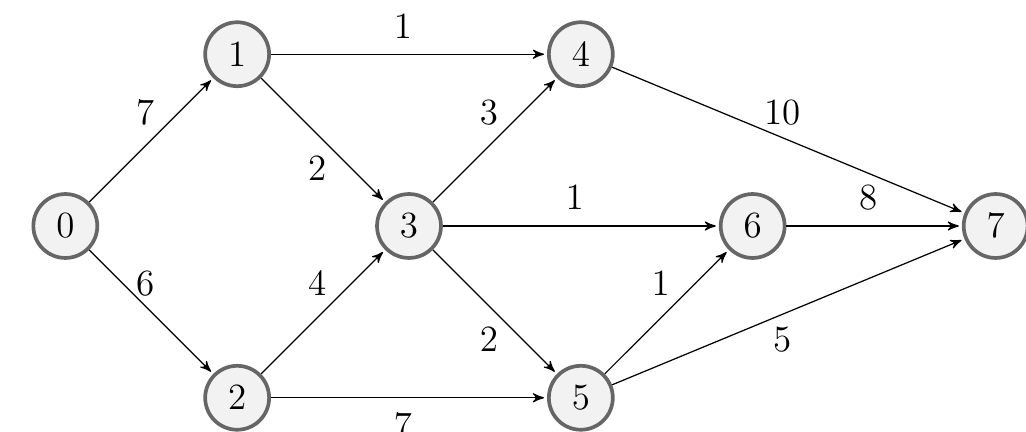
\includegraphics{01-introduction/../assets/ch_00/network_brandimarte_ex.png}

}

\caption{\label{fig-brandimarte_net}The shortest path}

\end{figure}%

We present an introduction to the solution of multi-stage optimization
problems. Starting from the dynamic programming algorithm, we consider
theoretical and computational aspects, mainly of deterministic problems,
and discuss how to generalize some of the results to Markovian decision
processes.

\begin{longtable}[]{@{}lc@{}}
\caption{The shortest path by exhaustion see
(\citeproc{ref-brandimarte2013numerical}{Brandimarte
2013}).}\label{tbl-brandimarte_paths}\tabularnewline
\toprule\noalign{}
Path & Cost \\
\midrule\noalign{}
\endfirsthead
\toprule\noalign{}
Path & Cost \\
\midrule\noalign{}
\endhead
\bottomrule\noalign{}
\endlastfoot
\(0 \to 1 \to 4 \to 7\) & 18 \\
\(0 \to 1 \to 3 \to 4 \to 7\) & 22 \\
\(0 \to 1 \to 3 \to 6 \to 7\) & 18 \\
\(0 \to 1 \to 3 \to 5 \to 6 \to 7\) & 20 \\
\(\mathbf{0 \to 1 \to 3 \to 5 \to 7}\) & \textbf{16} \\
\(0 \to 2 \to 3 \to 4 \to 7\) & 23 \\
\(0 \to 2 \to 3 \to 6 \to 7\) & 19 \\
\(0 \to 2 \to 3 \to 5 \to 6 \to 7\) & 21 \\
\(0 \to 2 \to 3 \to 5 \to 7\) & 17 \\
\(0 \to 2 \to 5 \to 6 \to 7\) & 22 \\
\(0 \to 2 \to 5 \to 7\) & 18 \\
\end{longtable}

The classic problem with which the essential ideas of dynamic
programming can be introduced is the optimal route problem (shortest
route considering distances,or cheapest route considering costs)
(\citeproc{ref-Bertsekas2005}{Bertsekas 2005};
\citeproc{ref-brandimarte2013numerical}{Brandimarte 2013}). A simple
version of this problem is shown schematically in
Figure~\ref{fig-brandimarte_net}. By exhaustion, we deploy the cost of
path in Table~\ref{tbl-brandimarte_paths}.

In this problem, the optimal route to go from the node labeled \(0\) to
the node labeled \(7\) is to be determined. The costs between each pair
of nodes connected by an arrow are represented by a number next to it.
For example, the cost to go from node 0 to node 2 is 6. The optimal
route will be the one for which the sum of their costs is minimum. This
optimal route can be obtained by an exhaustive enumeration; generating
all possible routes from node \(0\) to node \(7\) and choosing the
minimum cost route.

The optimal path is \[
  0 \to   1 \to 3 \to 5 \to  7,
\] with cost 16.

\bookmarksetup{startatroot}

\chapter{Introduction}\label{introduction}

Reinforcement Learning is part of a decades-long trend within artificial
intelligence and machine learning toward greater integration with
statistics, optimization, and other mathematical subjects. For example,
the ability of some reinforcement learning methods to learn with
parameterized approximators addresses the classical ``curse of
dimensionality'' in operations research and control theory. More
distinctively, reinforcement learning has also interacted strongly with
psychology and neuroscience, with substantial benefits going both ways.
Of all the forms of machine learning, reinforcement learning is the
closest to the kind of learning that humans and other animals do, and
many of the core algorithms of reinforcement learning were originally
inspired by biological learning systems.

\section{Trial-Error}\label{trial-error}

According to Richard S. Sutton and Andrew G. Barto Sutton and Barto
(\citeproc{ref-Sutton2018}{2018})--the first authors to use the
term--Reinforced Learning Reinforcement learning is about what to do,
that is, how to map situations to action so that we optimize a reward.
\textbf{The learner must discover which action yield the best reward by
trying them.} In the most general sense, action may not only affect
immediate reward but also the next situation and, through that, all
subsequent rewards.

\subsection{Sensation action and goal}\label{sensation-action-and-goal}

At the same time, Reinforcement Learning encloses a problem, a class of
solution methods, and the field that studies this problem and its
solutions. Its formalism is based on the theory of controlled dynamical
systems, with a strong focus on the optimal control of partially known
Markov decision processes. Then, the core idea consists of capturing the
essence of the problem when an agent learns through experience and
interaction to reach a goal. This agent can sense the state of its
environment to some extent and must be able to take action that affects
the state. The agent also must have a goal or goals related to the state
of the environment.

MDPs are designed to incorporate three essential elements: sensation,
action, and goal. Therefore, any approach suitable for solving such
problems should be considered a potential method for Reinforcement
Learning.

\section{Exploration-exploration dilemma and
uncertainty}\label{exploration-exploration-dilemma-and-uncertainty}

To obtain the best reward, the agent must prefer actions used in the
past and perceived as effective to produce a reward. However, to
discover such actions, the agent must try actions never used before. So,
there is a delicate trade-off between exploiting and exploring. The
agent has to exploit its knowledge to produce a reward but
simultaneously has to explore to improve its reward in the future. Here,
our dilemma is that neither exploration nor exploitation can be pursued
exclusively without failing the task.

Another essential aspect of reinforcement learning is that it
specifically deals with the entire process of a goal-directed agent
interacting with an uncertain environment. This aspect differs from many
approaches that only focus on subproblems rather than considering how
they might contribute to the bigger picture. For example, many machine
learning researchers have studied supervised Learning without specifying
how such an ability would ultimately be helpful. Other researchers have
developed planning theories with general goals without considering
planning's role in real-time decision-making or whether the predictive
models necessary for planning are well suited. Although these approaches
have produced valuable results, their focus on isolated subproblems
leads to significant limitations.

Reinforcement learning takes the opposite approach, beginning with a
fully interactive, goal-seeking agent. In reinforcement learning, the
agent has explicit goals, can sense aspects of their environment, and
can choose actions to influence its environment.

\section{Examples}\label{examples}

\begin{itemize}
\item
  A master chess player makes a move.
\item
  An adaptive controller adjusts parameters of a petroleum refinery's
  operation in real time.
\item
  A gazelle calf struggles to its feet minutes after being born.
\item
  A mobile robot decides whether it should enter a new room in search of
  more trash to collect or start trying to find its way back to its
  battery recharging station.
\item
  Phil prepares his breakfast
\end{itemize}

\section{The (possible) 4 elements of Reinforcement
Learning}\label{the-possible-4-elements-of-reinforcement-learning}

Given an agent, we identify four main element in a reinforcement
learning model:

\begin{quote}
a \textbf{policy}, a \textbf{reward}, a value function and (optionally)
a model of the \textbf{environment}.
\end{quote}

\begin{description}
\item[Policy]
A policy is as a set of actions that guide the agent to respond
according to its perception of the environment. It's like a set of
instructions that tell the agent what to do when it encounters a certain
situation. In general, policies may be stochastic, specifying
probabilities for each action.
\item[Reward]
The reward signal thus defines what are the good and bad events for the
agent. In a biological system, we might think of rewards as analogous to
the experiences of pleasure or pain. They are the immediate and defining
features of the problem faced by the agent. The reward signal is the
primary basis for altering the policy; if an action selected by the
policy is followed by low reward, then the policy may be changed to
select some other action in that situation in the future. In general,
reward signals may be stochastic functions of the state of the
environment and the actions taken.
\item[Value function]
Whereas the reward signal indicates what is good in the immediate sense,
a value function specifies what is good in the long run. In simple
terms, the value of a state represents the total reward an agent can
anticipate to receive in the future, beginning from that state. While
rewards reflect the immediate appeal of environmental states, values
signify the long-term appeal of states, considering the potential future
states and the rewards they offer. For example, a state might
consistently yield a low immediate reward but still have a high value
because it is regularly followed by other states that yield high
rewards. Alternatively, the opposite could also be true. Rewards can be
compared to pleasure (when high) and pain (when low). At the same time,
values represent a more precise and long-term assessment of how
satisfied or dissatisfied we are with the state of our environment. In a
sense, rewards are primary, whereas values, as predictions of rewards,
are secondary. Without rewards, there could be no values, and the only
purpose of estimating values is to achieve more rewards.

Action choices are made based on value judgments. We seek actions that
bring about states of highest value, not highest reward, because these
actions obtain the greatest amount of reward for us over the long run.
In fact, the most important component of almost all reinforcement
learning algorithms we consider is a method for efficiently estimating
values.
\item[Environment model]
The environment model is something that mimics the behavior of the
environment or, more generally, that allows inferences to be made about
how the environment will behave. For example, given a state and action,
the model might predict the resultant next state and next reward. Models
are used for planning. This means making decisions by considering
potential future situations before they occur. For our purposes, the
environment can be represented as a dynamic system through an ordinary
differential equation or a discrete finite difference equation.
\end{description}

\section{A toy RL-exmaple:
Tic-Tac-Toe}\label{a-toy-rl-exmaple-tic-tac-toe}

To illustrate the general idea of reinforcement learning and contrast it
with other ap- proaches, we next consider a single example in more
detail.

Consider the familiar child's game of tic-tac-toe.

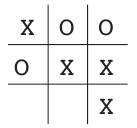
\includegraphics{02-introductionToRL/../assets/tic_tac_toe.jpeg}

Although the tic-tac-toe game is a simple problem, it cannot be
satisfactorily solved using classical techniques.

For instance, the classical ``\emph{minimax}'' solution from game theory
is not applicable here because it assumes the opponent's specific way of
playing. A \emph{minimax} player would never reach a game state from
which it could lose. Even if, in reality, it always won from that state
due to incorrect play by the opponent. The classical optimization
methods for sequential decision problems, like dynamic programming, can
find the best solution for any opponent. However, these methods need a
detailed description of the opponent as input, including the
probabilities of the opponent's moves in each board state.

Alternatively, this information can be estimated through experience,
such as playing numerous games against the opponent. The best approach
to this problem is to first learn a model of the opponent's behavior
with a certain level of confidence, and then use dynamic programming to
calculate an optimal solution based on the approximate opponent model.

Sutton and Barto (see pp.~9-12 \citeproc{ref-Sutton2018}{Sutton and
Barto 2018}) propose the following way to approach tic tac toe with
Reinforcement Learning:

\section*{Setup:}\label{setup}
\addcontentsline{toc}{section}{Setup:}

\markright{Setup:}

\begin{itemize}
\item
  First we would set up a table of numbers (or labels), one for each
  possible state of the game.
\item
  Each number will be the latest estimate of the probability of our
  winning from that state.
\item
  We treat this estimate as the state's value, and the whole table is
  the learned value function.
\item
  State \(A\) has higher value than state \(B\), or is considered
  `better' than state \(B\), if the current estimate of the probability
  of our winning from \(A\) is higher than it is from \(B\).
\item
  If we always play \(Xs\), then for all states with three \(Xs\) in a
  row the probability of winning is 1, because we have already won.
\item
  Similarly, for all states with three \(Os\) in a row, or that are
  filled up, the correct probability is 0--we cannot win from them.
\item
  We set the initial values of all the other states to \(0.5\),
  representing a guess that we have a 50\% chance of winning.
\end{itemize}

\section*{Training:}\label{training}
\addcontentsline{toc}{section}{Training:}

\markright{Training:}

We then play many games against the opponent.

To select our moves we examine the states that would result from each of
our possible moves (one for each blank space on the board) and look up
their current values in the table. Most of the time we move
greedily,selecting the move that leads to the state with greatest value,
that is, with the highest estimated probability of winning.

Occasionally, however, we select randomly from among the other moves
instead. These are called exploratory moves because they cause us to
experience states that we might otherwise never see.

A sequence of moves made and considered during a game can be diagrammed
as the following figure:

\begin{figure*}

\centering{

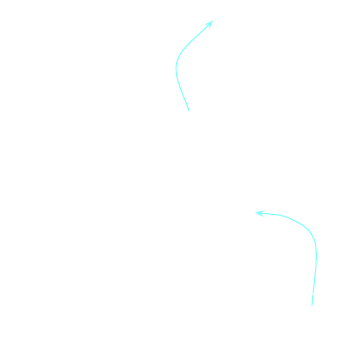
\includegraphics{02-introductionToRL/../assets/ch_00/diagram_sequence_tictactoe_play.png}

}

\caption{\label{fig-tic_tac_toc_diag}Figure taken from
(\citeproc{ref-Sutton2018}{Sutton and Barto 2018}). A sequence of
tic-tac-toe moves. Solid black lines represents moves taken during a
play. Dashed lines represent plausible but not taken moves. The \(*\)
symbol indicates the move currently estimated to be the best. Thus the
move \(e\) denotes an \emph{exploratory} move}

\end{figure*}%

\bookmarksetup{startatroot}

\chapter{Multi-armed Bandits}\label{multi-armed-bandits}

A very important feature distinguishing reinforcement learning from
other types of learning is that it uses training information to evaluate
the actions taken, rather than instruct by giving correct actions.

\section{\texorpdfstring{A \(k\)-armed Bandit
Problem}{A k-armed Bandit Problem}}\label{a-k-armed-bandit-problem}

We consider the following setup:

\begin{itemize}
\tightlist
\item
  You repeatedly face a choice among \(k\) different options or actions.
\item
  After a choice, you receive a numerical reward chosen from a
  stationary probability distribution that depends on the action you
  selected
\item
  Your goal is to maximize the total expected reward over a specific
  time period, such as 1000 action selections or time steps. The problem
  is named by analogy to a slot machine, or \texttt{one-armed\ bandit},
  except that it has \(k\) levers instead of one.
\end{itemize}

We denote the action selected on time step \(t\) as \(A_t\) and the
corresponding reward as \(R_t\). Each of the \(k\) actions has an
expected or mean reward given that that action is selected; let us call
this the value of that action.

The value then of an arbitrary action \(a\), denoted \(q_{*} (a)\), is
the expected reward given that \(a\) is selected:

\[
    q_{*}(a): = \mathbb{E} \left[ R_t | A_t =a\right].
\]

If you knew the value of each action, then we solve the \(k\)-armed
bandit problem---you would always
\texttt{select\ the\ action\ with\ highest\ value}.

We assume that you may not have precise knowledge of the action values,
although you may have some estimates. We denote this estimated value of
action \(a\) at time step \(t\) as \(Q_t(a)\). Thus, we would like that
\[
    Q_t(a) \approx q_{*}(a).
\]

If you maintain estimates of the action values, then at any time step
there is at least one action whose estimated value is greatest. We call
these the \emph{greedy} actions. When you select one of these actions,
we say that you are \emph{exploiting} your current knowledge of the
values of the actions. If instead you select one of the non-greedy
actions, then we say you are exploring, because this enables you to
improve your estimate of the non-greedy action's value.

Exploitation is the right thing to do to maximize the expected reward on
the one step, but exploration may produce the greater total reward in
the long run.

Reward is lower in the short run, during exploration, but higher in the
long run because after you have discovered the better actions, you can
exploit them many times. Because it is not possible both to explore and
to exploit with any single action selection, one often refers to the
``conflict'' between exploration and exploitation.

In any specific case, whether it is better to explore or exploit depends
in a complex way on the precise values of the estimates, uncertainties,
and the number of remaining steps. There are many sophisticated methods
for balancing exploration and exploitation for particular mathematical
formulations of the \(k\)-armed bandit and related problems.

However, most of these methods make strong assumptions about stationary
and prior knowledge that are either violated or impossible to verify in
most applications.

The guarantees of optimality or bounded loss for these methods offer
little comfort when the assumptions of their theory do not apply.

\section{Action-value Methods}\label{action-value-methods}

One natural way to estimate the value of a given action is by averaging
the rewards actually received. In mathematical symbols reads

\begin{equation}\phantomsection\label{eq-action_avering_kbandit}{
  Q_t(a):=
    \dfrac{
      \sum_{i=1}^{t-1}
        R_i \cdot \mathbb{1}_{A_{i} = a}
    }{\sum_{i=1}^{t-1} \mathbb{1}_{A_i=a}} .
}\end{equation}

Next we understand as greedy action as the action that results from
\begin{equation}\phantomsection\label{eq-greedy_action}{
  A_t := \underset{a}{\mathrm{argmax}} \ Q_t(a).
}\end{equation}

Greedy action selection always exploits current knowledge to maximize
immediate reward. It also only spends time sampling apparently superior
actions. A simple alternative is to behave greedily but occasionally,
with a small \(\epsilon\)-probability, select randomly from all the
actions with equal probability, regardless of the action-value
estimates. We call methods using this near-greedy action selection rule
\(\epsilon\)-greedy methods.

\section{The 10-armed Testbed}\label{the-10-armed-testbed}

To evaluate the relative effectiveness of the greedy and
\(\epsilon\)-greedy action-value methods, we compared them numerically
on a suite of test problems.

\subsection{Set up}\label{set-up}

\begin{tcolorbox}[enhanced jigsaw, bottomrule=.15mm, opacityback=0, breakable, colframe=quarto-callout-tip-color-frame, left=2mm, rightrule=.15mm, toprule=.15mm, leftrule=.75mm, arc=.35mm, colback=white]
\begin{minipage}[t]{5.5mm}
\textcolor{quarto-callout-tip-color}{\faLightbulb}
\end{minipage}%
\begin{minipage}[t]{\textwidth - 5.5mm}

\vspace{-3mm}\textbf{The experiment runs as follows.}\vspace{3mm}

\begin{itemize}
\item
  Consider a \(k\)-bandit problem with \(k=10\)
\item
  For each bandit problem, the action values
\end{itemize}

\[
  q_{*}(a) \sim \mathcal{N}(0,1)
\]

\begin{itemize}
\tightlist
\item
  Then when choosing an action \(A_t\) the corresponding reward \(R_t\)
  is sampling from a Gaussian distribution \[
  R_t \sim \mathcal{N}(q_{*}(A_t), 1)  
  \]
\end{itemize}

\end{minipage}%
\end{tcolorbox}

\begin{codelisting}

\caption{\texttt{k\_armed\_testbed.py}}

\begin{Shaded}
\begin{Highlighting}[]
\CommentTok{\#k\_armed\_testbed.py}
\ImportTok{import}\NormalTok{ numpy }\ImportTok{as}\NormalTok{ np}
\ImportTok{from}\NormalTok{ matplotlib }\ImportTok{import}\NormalTok{ pyplot }\ImportTok{as}\NormalTok{ plt}


\CommentTok{\# Randomly sample mean reward for each action}
\NormalTok{means }\OperatorTok{=}\NormalTok{ np.random.normal(size}\OperatorTok{=}\NormalTok{(}\DecValTok{10}\NormalTok{, ))}

\CommentTok{\# Generate sample data based on normal distribution}
\NormalTok{data }\OperatorTok{=}\NormalTok{ [np.random.normal(mean, }\FloatTok{1.0}\NormalTok{, }\DecValTok{2000}\NormalTok{) }\ControlFlowTok{for}\NormalTok{ mean }\KeywordTok{in}\NormalTok{ means]}

\CommentTok{\# Create violin plot}
\NormalTok{plt.figure(figsize}\OperatorTok{=}\NormalTok{(}\DecValTok{8}\NormalTok{, }\DecValTok{6}\NormalTok{), dpi}\OperatorTok{=}\DecValTok{150}\NormalTok{)}
\NormalTok{plt.violinplot(}
\NormalTok{  dataset}\OperatorTok{=}\NormalTok{data,}
\NormalTok{  showextrema}\OperatorTok{=}\VariableTok{False}\NormalTok{,}
\NormalTok{  showmeans}\OperatorTok{=}\VariableTok{False}\NormalTok{,}
\NormalTok{  points}\OperatorTok{=}\DecValTok{2000}
\NormalTok{)}

\CommentTok{\# Draw mean marks}
\ControlFlowTok{for}\NormalTok{ i, mean }\KeywordTok{in} \BuiltInTok{enumerate}\NormalTok{(means):}
\NormalTok{    idx }\OperatorTok{=}\NormalTok{ i }\OperatorTok{+} \DecValTok{1}
\NormalTok{    plt.plot([idx }\OperatorTok{{-}} \FloatTok{0.3}\NormalTok{, idx }\OperatorTok{+} \FloatTok{0.3}\NormalTok{], [mean, mean],}
\NormalTok{             c}\OperatorTok{=}\StringTok{\textquotesingle{}black\textquotesingle{}}\NormalTok{,}
\NormalTok{             linewidth}\OperatorTok{=}\DecValTok{1}\NormalTok{)}
\NormalTok{    plt.text(idx }\OperatorTok{+} \FloatTok{0.2}\NormalTok{, mean }\OperatorTok{{-}} \FloatTok{0.2}\NormalTok{, }
\NormalTok{             s}\OperatorTok{=}\SpecialStringTok{f"$q\_*(}\SpecialCharTok{\{}\NormalTok{idx}\SpecialCharTok{\}}\SpecialStringTok{)$"}\NormalTok{,}
\NormalTok{             fontsize}\OperatorTok{=}\DecValTok{8}\NormalTok{)}

\CommentTok{\# Draw 0{-}value dashed line}
\NormalTok{plt.plot(np.arange(}\DecValTok{0}\NormalTok{, }\DecValTok{12}\NormalTok{), np.zeros(}\DecValTok{12}\NormalTok{), }
\NormalTok{            c}\OperatorTok{=}\StringTok{\textquotesingle{}gray\textquotesingle{}}\NormalTok{, }
\NormalTok{            linewidth}\OperatorTok{=}\FloatTok{0.5}\NormalTok{,}
\NormalTok{            linestyle}\OperatorTok{=}\NormalTok{(}\DecValTok{5}\NormalTok{, (}\DecValTok{20}\NormalTok{, }\DecValTok{10}\NormalTok{)))}
\NormalTok{plt.tick\_params(axis}\OperatorTok{=}\StringTok{\textquotesingle{}both\textquotesingle{}}\NormalTok{, labelsize}\OperatorTok{=}\DecValTok{10}\NormalTok{)}
\NormalTok{plt.xticks(np.arange(}\DecValTok{1}\NormalTok{, }\DecValTok{11}\NormalTok{))}

\CommentTok{\# get rid of the frame}
\ControlFlowTok{for}\NormalTok{ i, spine }\KeywordTok{in} \BuiltInTok{enumerate}\NormalTok{(plt.gca().spines.values()):}
    \ControlFlowTok{if}\NormalTok{ i }\OperatorTok{==} \DecValTok{2}\NormalTok{: }\ControlFlowTok{continue}
\NormalTok{    spine.set\_visible(}\VariableTok{False}\NormalTok{)}
    

\CommentTok{\# Draw labels}
\NormalTok{label\_font }\OperatorTok{=}\NormalTok{ \{}
    \StringTok{\textquotesingle{}fontsize\textquotesingle{}}\NormalTok{: }\DecValTok{12}\NormalTok{,}
    \StringTok{\textquotesingle{}fontweight\textquotesingle{}}\NormalTok{: }\StringTok{\textquotesingle{}bold\textquotesingle{}}
\NormalTok{\}}

\NormalTok{plt.xlabel(}\StringTok{\textquotesingle{}Action\textquotesingle{}}\NormalTok{, fontdict}\OperatorTok{=}\NormalTok{label\_font)}
\NormalTok{plt.ylabel(}\StringTok{\textquotesingle{}Reward distribution\textquotesingle{}}\NormalTok{, fontdict}\OperatorTok{=}\NormalTok{label\_font)}
\NormalTok{plt.margins(}\DecValTok{0}\NormalTok{)}

\NormalTok{plt.tight\_layout()}
\NormalTok{plt.show()}
\end{Highlighting}
\end{Shaded}

\end{codelisting}

We consider a set of 2000 randomly generated \(k\)-armed bandit problems
with \(k\) = 10. For each bandit problem, such as the one shown in the
output of the above code. The action values,
\(q_{*} (a), a = 1, . . . , 10\), were selected according to a normal
(Gaussian) distribution with mean 0 and variance 1. Thus when we apply a
learning method to this problem, the selected action \(A_t\) a time step
\(t\) the regarding reward \(R_t\) is sampling from a normal
distribution \[
  R_{t} \sim \mathcal{N}(q_{*}(A_t), 1).
\] Sutton and Barto (\citeproc{ref-Sutton2018}{Sutton and Barto 2018,
28}) calls this suite of test tasks the 10-armed test-bed. By using this
suit of benchmarks, we can measure the performance of any learning
method. In fact we also can observe its behavior while the learning
improves with experience of 1000 time steps, when it is applied to a
selected bandit of this bed. This makes up one run. Thus, if we
\textbf{iterate 2000} independent runs, each with different bandit
problem, we can obtain a measure of learning algorithm's average
behavior.

Next we code functions to deploy the above experiment with
\(\epsilon\)-greedy actions

\begin{codelisting}

\caption{\texttt{utils.py}}

\begin{Shaded}
\begin{Highlighting}[]
\ImportTok{from}\NormalTok{ typing }\ImportTok{import}\NormalTok{ Any}
\ImportTok{import}\NormalTok{ matplotlib.pyplot }\ImportTok{as}\NormalTok{ plt}
\ImportTok{import}\NormalTok{ numpy }\ImportTok{as}\NormalTok{ np}
\ImportTok{from}\NormalTok{ numpy }\ImportTok{import}\NormalTok{ dtype, ndarray, signedinteger}


\CommentTok{\# Get the action with the max Q value}
\KeywordTok{def}\NormalTok{ get\_argmax(G:np.ndarray) }\OperatorTok{{-}\textgreater{}}\NormalTok{ ndarray[Any, dtype[signedinteger[Any]]]:}
\NormalTok{    candidates }\OperatorTok{=}\NormalTok{ np.argwhere(G }\OperatorTok{==}\NormalTok{ G.}\BuiltInTok{max}\NormalTok{()).flatten()}
    \CommentTok{\# return the only index if there\textquotesingle{}s only one max}
    \ControlFlowTok{if} \BuiltInTok{len}\NormalTok{(candidates) }\OperatorTok{==} \DecValTok{1}\NormalTok{:}
        \ControlFlowTok{return}\NormalTok{ candidates[}\DecValTok{0}\NormalTok{]}
    \ControlFlowTok{else}\NormalTok{:}
        \CommentTok{\# instead break the tie randomly}
        \ControlFlowTok{return}\NormalTok{ np.random.choice(candidates)}


\CommentTok{\# Select arm and get the reward}
\KeywordTok{def}\NormalTok{ bandit(q\_star:np.ndarray, }
\NormalTok{           act:}\BuiltInTok{int}\NormalTok{) }\OperatorTok{{-}\textgreater{}} \BuiltInTok{tuple}\NormalTok{:}
\NormalTok{    real\_rewards }\OperatorTok{=}\NormalTok{ np.random.normal(q\_star, }\FloatTok{1.0}\NormalTok{)}
    \CommentTok{\# optim\_choice = int(real\_rewards[act] == real\_rewards.max())}
\NormalTok{    optim\_choice }\OperatorTok{=} \BuiltInTok{int}\NormalTok{(q\_star[act] }\OperatorTok{==}\NormalTok{ q\_star.}\BuiltInTok{max}\NormalTok{())}
    \ControlFlowTok{return}\NormalTok{ real\_rewards[act], optim\_choice}
\end{Highlighting}
\end{Shaded}

\end{codelisting}

Please save the above script as \texttt{utils.py} in the firs level of
the regrding project such that we can imported by the ist name fora
example by \texttt{from\ utils\ import\ bandit,\ plots}

\section{Incremental Implementation}\label{incremental-implementation}

Certainly! To express a more efficient method for estimating action
values, we focus on using an \textbf{incremental update formula} rather
than recalculating the average based on all past observations. The goal
is to maintain a constant memory footprint and fixed computation per
time step.

\subsection{Incremental Update Formula for Action-Value
Estimation}\label{incremental-update-formula-for-action-value-estimation}

Let \(R_i\) denote the reward received after the \(i\)-th selection of
the action.\(Q_n\) denote the estimate of the action value after the
action has been chosen \(n-1\) times.

Instead of computing \(Q_n\) as the sample average of all observed
rewards (which requires storing and summing all rewards), we use the
\textbf{incremental formula}:

\[
    Q_n = Q_{n-1} + \alpha \left(R_n - Q_{n-1}\right) 
\]

Where: \(Q_{n-1}\) is the previous estimate of the action value. \(R_n\)
is the reward received on the \(n\)-th selection. \(\alpha\) is a
\textbf{constant step size}, often set as \(\dfrac{1}{n}\) to mimic the
behavior of sample averaging when the number of observations grows.

\subsection{Derivation of the Incremental
Formula}\label{derivation-of-the-incremental-formula}

\begin{enumerate}
\def\labelenumi{\arabic{enumi}.}
\item
  Start with the definition of the action value as the sample mean:
  \(\displaystyle Q_n =\dfrac{1}{n} \sum_{i=1}^{n} R_i\)
\item
  Express \(Q_n\) in terms of \(Q_{n-1}\): \[
  Q_n = \frac{1}{n}
  \left[ \sum_{i=1}^{n-1} R_i + R_n \right]
  \]
\end{enumerate}

This can be rearranged as: \[
        Q_n = \frac{n-1}{n} \cdot Q_{n-1} +
    \frac{1}{n} \cdot R_n. 
\]

\begin{enumerate}
\def\labelenumi{\arabic{enumi}.}
\setcounter{enumi}{2}
\tightlist
\item
  Notice that \(\displaystyle
      \frac{n-1}{n} \cdot Q_{n-1} = Q_{n-1} - \frac{1}{n}\cdot Q_{n-1}\),
  so: \[ 
      Q_n = Q_{n-1} + \frac{1}{n} \left(R_n -Q_{n-1}\right)
  \]
\end{enumerate}

Here, \(\alpha = \dfrac{1}{n}\) adapts to the number of observations,
ensuring the update balances the influence of new and past rewards.

\subsection{Advantages of the Incremental
Method}\label{advantages-of-the-incremental-method}

\begin{itemize}
\tightlist
\item
  \textbf{Constant Memory}: The method only requires storing \(Q_{n-1}\)
  and \(R_n\), avoiding the need to keep all past rewards.
\item
  \textbf{Fixed Computation}: Each update involves a fixed, small number
  of operations, regardless of \(n\).
\end{itemize}

This approach efficiently updates the action-value estimate with minimal
resources, making it suitable for online learning algorithms and
scenarios where computational efficiency is critical.

\begin{figure}[H]

{\centering 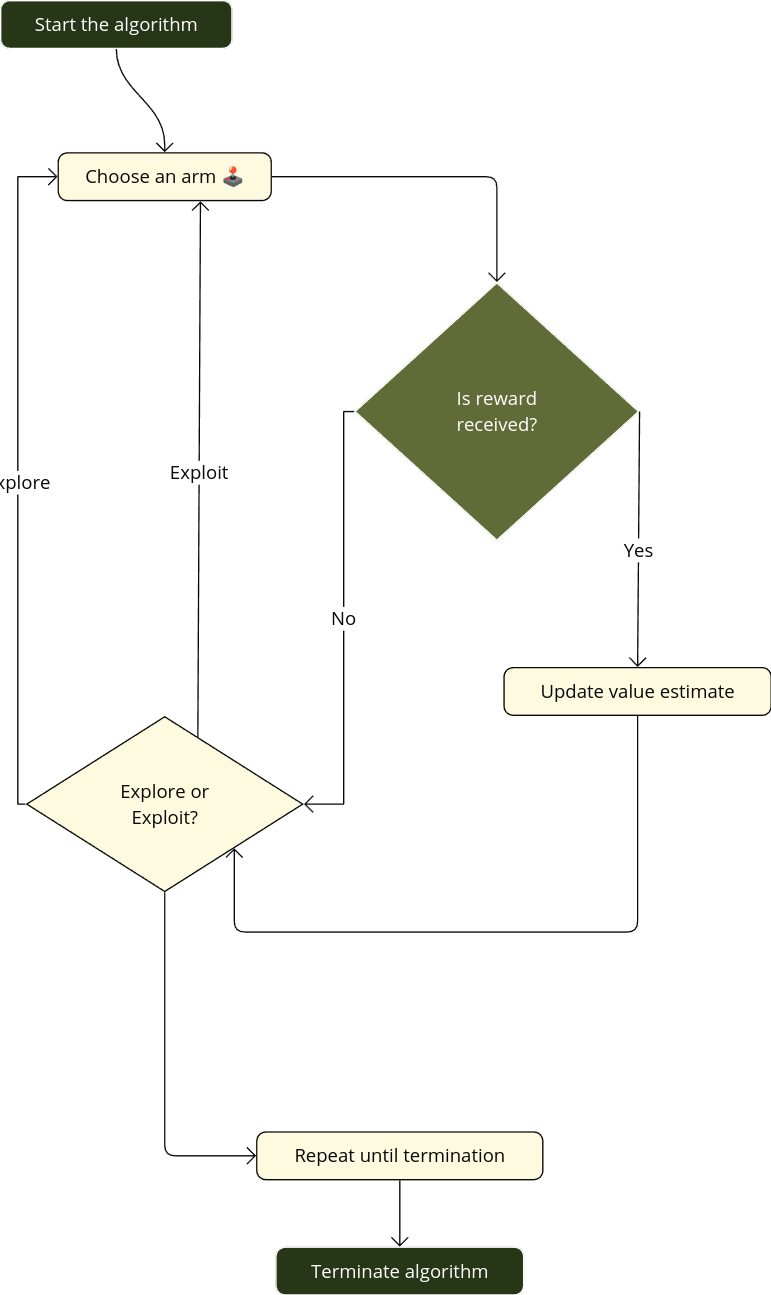
\includegraphics{assets/ch_03/mab_simple_algorithm.png}

}

\caption{Incremental algorithm}

\end{figure}%

Bellow a python implementation.

\begin{codelisting}

\caption{\texttt{example\_2\_2\_bandits\_algo.py}}

\begin{Shaded}
\begin{Highlighting}[]
\ImportTok{import}\NormalTok{ numpy }\ImportTok{as}\NormalTok{ np}
\ImportTok{import}\NormalTok{ matplotlib}
\ImportTok{import}\NormalTok{ matplotlib.pyplot }\ImportTok{as}\NormalTok{ plt}
\NormalTok{matplotlib.use(}\StringTok{\textquotesingle{}qt5agg\textquotesingle{}}\NormalTok{)}
\ImportTok{import}\NormalTok{ pickle}

\ImportTok{from}\NormalTok{ utils }\ImportTok{import}\NormalTok{ get\_argmax, bandit}

\CommentTok{\#SEED = 123456}
\CommentTok{\#np.random.seed(SEED)}

\CommentTok{\# running the k{-}armed bandit algorithm}
\KeywordTok{def}\NormalTok{ run\_bandit(K:}\BuiltInTok{int}\NormalTok{, }
\NormalTok{            q\_star:np.ndarray,}
\NormalTok{            rewards:np.ndarray,}
\NormalTok{            optim\_acts\_ratio:np.ndarray,}
\NormalTok{            epsilon:}\BuiltInTok{float}\NormalTok{, }
\NormalTok{            num\_steps:}\BuiltInTok{int}\OperatorTok{=}\DecValTok{1000}\NormalTok{) }\OperatorTok{{-}\textgreater{}} \VariableTok{None}\NormalTok{:}
    
\NormalTok{    Q }\OperatorTok{=}\NormalTok{ np.zeros(K)     }\CommentTok{\# Initialize Q values}
\NormalTok{    N }\OperatorTok{=}\NormalTok{ np.zeros(K)     }\CommentTok{\# The number of times each action been selected}
\NormalTok{    ttl\_optim\_acts }\OperatorTok{=} \DecValTok{0}

    \ControlFlowTok{for}\NormalTok{ i }\KeywordTok{in} \BuiltInTok{range}\NormalTok{(num\_steps):}
        \CommentTok{\# get action}
\NormalTok{        A }\OperatorTok{=} \VariableTok{None}
        \ControlFlowTok{if}\NormalTok{ np.random.random() }\OperatorTok{\textgreater{}}\NormalTok{ epsilon:}
\NormalTok{            A }\OperatorTok{=}\NormalTok{ get\_argmax(Q)}
        \ControlFlowTok{else}\NormalTok{:}
\NormalTok{            A }\OperatorTok{=}\NormalTok{ np.random.randint(}\DecValTok{0}\NormalTok{, K)}
        
\NormalTok{        R, is\_optim }\OperatorTok{=}\NormalTok{ bandit(q\_star, A)}
\NormalTok{        N[A] }\OperatorTok{+=} \DecValTok{1}
\NormalTok{        Q[A] }\OperatorTok{+=}\NormalTok{ (R }\OperatorTok{{-}}\NormalTok{ Q[A]) }\OperatorTok{/}\NormalTok{ N[A]}

\NormalTok{        ttl\_optim\_acts }\OperatorTok{+=}\NormalTok{ is\_optim}
\NormalTok{        rewards[i] }\OperatorTok{=}\NormalTok{ R}
\NormalTok{        optim\_acts\_ratio[i] }\OperatorTok{=}\NormalTok{ ttl\_optim\_acts }\OperatorTok{/}\NormalTok{ (i }\OperatorTok{+} \DecValTok{1}\NormalTok{)}


\ControlFlowTok{if} \VariableTok{\_\_name\_\_} \OperatorTok{==} \StringTok{"\_\_main\_\_"}\NormalTok{:}

    \CommentTok{\# Initializing the hyperparameters}
\NormalTok{    K }\OperatorTok{=} \DecValTok{10}  \CommentTok{\# Number of arms}
\NormalTok{    epsilons }\OperatorTok{=}\NormalTok{ [}\FloatTok{0.0}\NormalTok{, }\FloatTok{0.01}\NormalTok{, }\FloatTok{0.1}\NormalTok{]}
\NormalTok{    num\_steps }\OperatorTok{=} \DecValTok{1000}
\NormalTok{    total\_rounds }\OperatorTok{=} \DecValTok{1000}

    \CommentTok{\# Initialize the environment}
\NormalTok{    q\_star }\OperatorTok{=}\NormalTok{ np.random.normal(loc}\OperatorTok{=}\DecValTok{0}\NormalTok{, scale}\OperatorTok{=}\FloatTok{1.0}\NormalTok{, size}\OperatorTok{=}\NormalTok{K)}
\NormalTok{    rewards }\OperatorTok{=}\NormalTok{ np.zeros(shape}\OperatorTok{=}\NormalTok{(}\BuiltInTok{len}\NormalTok{(epsilons), total\_rounds, num\_steps))}
\NormalTok{    optim\_acts\_ratio }\OperatorTok{=}\NormalTok{ np.zeros(shape}\OperatorTok{=}\NormalTok{(}\BuiltInTok{len}\NormalTok{(epsilons), total\_rounds, num\_steps))}
    
    \CommentTok{\# Run the k{-}armed bandits alg.}
    \ControlFlowTok{for}\NormalTok{ i, epsilon }\KeywordTok{in} \BuiltInTok{enumerate}\NormalTok{(epsilons):}
        \ControlFlowTok{for}\NormalTok{ curr\_round }\KeywordTok{in} \BuiltInTok{range}\NormalTok{(total\_rounds):}
\NormalTok{            run\_bandit(K, q\_star, }
\NormalTok{                       rewards[i, curr\_round], }
\NormalTok{                       optim\_acts\_ratio[i, curr\_round], }
\NormalTok{                       epsilon, }
\NormalTok{                       num\_steps)}
    
\NormalTok{    rewards }\OperatorTok{=}\NormalTok{ rewards.mean(axis}\OperatorTok{=}\DecValTok{1}\NormalTok{)}
\NormalTok{    optim\_acts\_ratio }\OperatorTok{=}\NormalTok{ optim\_acts\_ratio.mean(axis}\OperatorTok{=}\DecValTok{1}\NormalTok{)}

\NormalTok{    record }\OperatorTok{=}\NormalTok{ \{}
        \StringTok{\textquotesingle{}hyper\_params\textquotesingle{}}\NormalTok{: epsilons, }
        \StringTok{\textquotesingle{}rewards\textquotesingle{}}\NormalTok{: rewards,}
        \StringTok{\textquotesingle{}optim\_acts\_ratio\textquotesingle{}}\NormalTok{: optim\_acts\_ratio}
\NormalTok{    \}}

\NormalTok{    fig\_01, ax\_01 }\OperatorTok{=}\NormalTok{ plt.subplots()}
\NormalTok{    fig\_02, ax\_02 }\OperatorTok{=}\NormalTok{ plt.subplots()}
    \ControlFlowTok{for}\NormalTok{ i, ratio }\KeywordTok{in} \BuiltInTok{enumerate}\NormalTok{(optim\_acts\_ratio):}
\NormalTok{        ax\_01.plot(}
\NormalTok{                ratio,}
\NormalTok{                label}\OperatorTok{=}\VerbatimStringTok{r\textquotesingle{}$\textbackslash{}epsilon=}\SpecialCharTok{\{epsilon\_i\}}\VerbatimStringTok{$\textquotesingle{}}\NormalTok{.}\BuiltInTok{format}\NormalTok{(epsilon\_i}\OperatorTok{=}\NormalTok{epsilons[i])}
\NormalTok{        )}
    
    \ControlFlowTok{for}\NormalTok{ i, reward }\KeywordTok{in} \BuiltInTok{enumerate}\NormalTok{(rewards):}
\NormalTok{        ax\_02.plot(}
\NormalTok{                reward,}
\NormalTok{                label}\OperatorTok{=}\VerbatimStringTok{r\textquotesingle{}$\textbackslash{}epsilon=}\SpecialCharTok{\{epsilon\_i\}}\VerbatimStringTok{$\textquotesingle{}}\NormalTok{.}\BuiltInTok{format}\NormalTok{(epsilon\_i}\OperatorTok{=}\NormalTok{epsilons[i])}
\NormalTok{                )}
\NormalTok{    ax\_01.set\_xlabel(}\VerbatimStringTok{r\textquotesingle{}$t$\textquotesingle{}}\NormalTok{, fontsize}\OperatorTok{=}\DecValTok{12}\NormalTok{)}
\NormalTok{    ax\_01.set\_ylabel(}\VerbatimStringTok{r\textquotesingle{}Optimal Action\textquotesingle{}}\NormalTok{, fontsize}\OperatorTok{=}\DecValTok{12}\NormalTok{)}
\NormalTok{    ax\_01.legend(loc}\OperatorTok{=}\StringTok{\textquotesingle{}best\textquotesingle{}}\NormalTok{)}
\NormalTok{    ax\_02.set\_xlabel(}\VerbatimStringTok{r\textquotesingle{}$t$\textquotesingle{}}\NormalTok{, fontsize}\OperatorTok{=}\DecValTok{12}\NormalTok{)}
\NormalTok{    ax\_02.set\_ylabel(}\VerbatimStringTok{r\textquotesingle{}Reward\textquotesingle{}}\NormalTok{, fontsize}\OperatorTok{=}\DecValTok{12}\NormalTok{)}
\NormalTok{    ax\_02.legend(loc}\OperatorTok{=}\StringTok{\textquotesingle{}best\textquotesingle{}}\NormalTok{)}
\NormalTok{    plt.show()}
    
    \CommentTok{\# with open(\textquotesingle{}./history/record.pkl\textquotesingle{}, \textquotesingle{}wb\textquotesingle{}) as f:}
    \CommentTok{\#     pickle.dump(record, f)}
\end{Highlighting}
\end{Shaded}

\end{codelisting}

\section{Tracking a Nonstationary
Problem}\label{tracking-a-nonstationary-problem}

The averaging methods we have discussed are suitable for stationary
bandit problems, where the reward probabilities remain constant over
time. However, in reinforcement learning, we often encounter
non-stationary problems where it makes more sense to give greater weight
to recent rewards than to rewards from a long time ago. One popular
approach to achieve this is by using a constant step-size parameter.

\#TODO: Formulation with constant alpha and implications

\section{Optimistic Initial Values}\label{optimistic-initial-values}

\begin{codelisting}

\caption{\texttt{example\_2\_3\_OIV.py}}

\begin{Shaded}
\begin{Highlighting}[]
\ImportTok{import}\NormalTok{ numpy }\ImportTok{as}\NormalTok{ np}
\ImportTok{import}\NormalTok{ matplotlib.pyplot }\ImportTok{as}\NormalTok{ plt}
\ImportTok{import}\NormalTok{ pickle}

\ImportTok{from}\NormalTok{ utils }\ImportTok{import}\NormalTok{ get\_argmax, bandit}

\NormalTok{SEED }\OperatorTok{=} \DecValTok{200}
\NormalTok{np.random.seed(SEED)}


\CommentTok{\# running the k{-}armed bandit algorithm}
\KeywordTok{def}\NormalTok{ run\_bandit(K: }\BuiltInTok{int}\NormalTok{,}
\NormalTok{            q\_star: np.ndarray,}
\NormalTok{            rewards: np.ndarray,}
\NormalTok{            optim\_acts\_ratio: np.ndarray,}
\NormalTok{            epsilon: }\BuiltInTok{float}\NormalTok{,}
\NormalTok{            num\_steps: }\BuiltInTok{int}\OperatorTok{=}\DecValTok{1000}\NormalTok{,}
\NormalTok{            init\_val: }\BuiltInTok{int}\OperatorTok{=}\DecValTok{0}
\NormalTok{) }\OperatorTok{{-}\textgreater{}} \VariableTok{None}\NormalTok{:}
\NormalTok{    Q }\OperatorTok{=}\NormalTok{ np.ones(K) }\OperatorTok{*}\NormalTok{ init\_val   }\CommentTok{\# Initial Q values with OIV}
\NormalTok{    ttl\_optim\_acts }\OperatorTok{=} \DecValTok{0}
\NormalTok{    alpha }\OperatorTok{=} \FloatTok{0.1}

    \ControlFlowTok{for}\NormalTok{ i }\KeywordTok{in} \BuiltInTok{range}\NormalTok{(num\_steps):}
        \CommentTok{\# get action}
\NormalTok{        A }\OperatorTok{=} \VariableTok{None}
        \ControlFlowTok{if}\NormalTok{ np.random.random() }\OperatorTok{\textgreater{}}\NormalTok{ epsilon:}
\NormalTok{            A }\OperatorTok{=}\NormalTok{ get\_argmax(Q)}
        \ControlFlowTok{else}\NormalTok{:}
\NormalTok{            A }\OperatorTok{=}\NormalTok{ np.random.randint(}\DecValTok{0}\NormalTok{, K)}
        
\NormalTok{        R, is\_optim }\OperatorTok{=}\NormalTok{ bandit(q\_star, A)}
\NormalTok{        Q[A] }\OperatorTok{+=}\NormalTok{ alpha }\OperatorTok{*}\NormalTok{ (R }\OperatorTok{{-}}\NormalTok{ Q[A])}

\NormalTok{        ttl\_optim\_acts }\OperatorTok{+=}\NormalTok{ is\_optim}
\NormalTok{        rewards[i] }\OperatorTok{=}\NormalTok{ R}
\NormalTok{        optim\_acts\_ratio[i] }\OperatorTok{=}\NormalTok{ ttl\_optim\_acts }\OperatorTok{/}\NormalTok{ (i }\OperatorTok{+} \DecValTok{1}\NormalTok{)}


\ControlFlowTok{if} \VariableTok{\_\_name\_\_} \OperatorTok{==} \StringTok{"\_\_main\_\_"}\NormalTok{:}

    \CommentTok{\# Initializing the hyper{-}parameters}
\NormalTok{    K }\OperatorTok{=} \DecValTok{10} \CommentTok{\# Number of arms}
\NormalTok{    epsilons }\OperatorTok{=}\NormalTok{ [}\FloatTok{0.1}\NormalTok{, }\FloatTok{0.0}\NormalTok{]}
\NormalTok{    init\_vals }\OperatorTok{=}\NormalTok{ [}\FloatTok{0.0}\NormalTok{, }\FloatTok{5.0}\NormalTok{]}
\NormalTok{    num\_steps }\OperatorTok{=} \DecValTok{1000}
\NormalTok{    total\_rounds }\OperatorTok{=} \DecValTok{2000}

    \CommentTok{\# Initialize the environment}
\NormalTok{    q\_star }\OperatorTok{=}\NormalTok{ np.random.normal(loc}\OperatorTok{=}\DecValTok{0}\NormalTok{, scale}\OperatorTok{=}\FloatTok{1.0}\NormalTok{, size}\OperatorTok{=}\NormalTok{K)}
\NormalTok{    rewards }\OperatorTok{=}\NormalTok{ np.zeros(shape}\OperatorTok{=}\NormalTok{(}\BuiltInTok{len}\NormalTok{(epsilons), total\_rounds, num\_steps))}
\NormalTok{    optim\_acts\_ratio }\OperatorTok{=}\NormalTok{ np.zeros(shape}\OperatorTok{=}\NormalTok{(}\BuiltInTok{len}\NormalTok{(epsilons), total\_rounds, num\_steps))}
    
    \CommentTok{\# Run the k{-}armed bandits alg.}
    \ControlFlowTok{for}\NormalTok{ i, (epsilon, init\_val) }\KeywordTok{in} \BuiltInTok{enumerate}\NormalTok{(}\BuiltInTok{zip}\NormalTok{(epsilons, init\_vals)):}
        \ControlFlowTok{for}\NormalTok{ curr\_round }\KeywordTok{in} \BuiltInTok{range}\NormalTok{(total\_rounds):}
\NormalTok{            run\_bandit(K, q\_star, }
\NormalTok{                       rewards[i, curr\_round], }
\NormalTok{                       optim\_acts\_ratio[i, curr\_round], }
\NormalTok{                       epsilon}\OperatorTok{=}\NormalTok{epsilon, }
\NormalTok{                       num\_steps}\OperatorTok{=}\NormalTok{num\_steps,}
\NormalTok{                       init\_val}\OperatorTok{=}\NormalTok{init\_val)}
    
\NormalTok{    rewards }\OperatorTok{=}\NormalTok{ rewards.mean(axis}\OperatorTok{=}\DecValTok{1}\NormalTok{)}
\NormalTok{    optim\_acts\_ratio }\OperatorTok{=}\NormalTok{ optim\_acts\_ratio.mean(axis}\OperatorTok{=}\DecValTok{1}\NormalTok{)}

\NormalTok{    record }\OperatorTok{=}\NormalTok{ \{}
        \StringTok{\textquotesingle{}hyper\_params\textquotesingle{}}\NormalTok{: [epsilons, init\_vals], }
        \StringTok{\textquotesingle{}rewards\textquotesingle{}}\NormalTok{: rewards,}
        \StringTok{\textquotesingle{}optim\_acts\_ratio\textquotesingle{}}\NormalTok{: optim\_acts\_ratio}
\NormalTok{    \}}

    \ControlFlowTok{for}\NormalTok{ vals }\KeywordTok{in}\NormalTok{ rewards:}
\NormalTok{        plt.plot(vals)}
\NormalTok{    plt.show()}
    \CommentTok{\# with open(\textquotesingle{}./history/OIV\_record.pkl\textquotesingle{}, \textquotesingle{}wb\textquotesingle{}) as f:}
    \CommentTok{\#     pickle.dump(record, f)}
\end{Highlighting}
\end{Shaded}

\end{codelisting}

\section{Upper-Confidence-Bound Action
Selection}\label{upper-confidence-bound-action-selection}

\begin{codelisting}

\caption{\texttt{example\_2\_4\_UCB.py}}

\begin{Shaded}
\begin{Highlighting}[]
\ImportTok{from}\NormalTok{ typing }\ImportTok{import}\NormalTok{ Any}
\ImportTok{import}\NormalTok{ numpy }\ImportTok{as}\NormalTok{ np}
\ImportTok{import}\NormalTok{ matplotlib.pyplot }\ImportTok{as}\NormalTok{ plt}
\ImportTok{import}\NormalTok{ pickle}
\ImportTok{from}\NormalTok{ numpy }\ImportTok{import}\NormalTok{ dtype, ndarray}
\ImportTok{from}\NormalTok{ tqdm }\ImportTok{import}\NormalTok{ tqdm}
\ImportTok{from}\NormalTok{ utils }\ImportTok{import}\NormalTok{ get\_argmax, bandit}

\NormalTok{SEED }\OperatorTok{=} \DecValTok{200}
\NormalTok{np.random.seed(SEED)}


\CommentTok{\# running the k{-}armed bandit algorithm}
\KeywordTok{def}\NormalTok{ run\_bandit(}
\NormalTok{        K: }\BuiltInTok{int}\NormalTok{,}
\NormalTok{        q\_star: np.ndarray,}
\NormalTok{        rewards: np.ndarray,}
\NormalTok{        optim\_acts\_ratio: np.ndarray,}
\NormalTok{        epsilon: }\BuiltInTok{float}\NormalTok{,}
\NormalTok{        num\_steps: }\BuiltInTok{int} \OperatorTok{=} \DecValTok{1000}
\NormalTok{        ) }\OperatorTok{{-}\textgreater{}} \VariableTok{None}\NormalTok{:}
\NormalTok{    Q }\OperatorTok{=}\NormalTok{ np.zeros(K)}
\NormalTok{    N }\OperatorTok{=}\NormalTok{ np.zeros(K)  }\CommentTok{\# The number of times each action been selected}
\NormalTok{    ttl\_optim\_acts }\OperatorTok{=} \DecValTok{0}
    
    \ControlFlowTok{for}\NormalTok{ i }\KeywordTok{in} \BuiltInTok{range}\NormalTok{(num\_steps):}
\NormalTok{        A }\OperatorTok{=} \VariableTok{None}
        \CommentTok{\# Get action}
        \ControlFlowTok{if}\NormalTok{ np.random.random() }\OperatorTok{\textgreater{}}\NormalTok{ epsilon:}
\NormalTok{            A }\OperatorTok{=}\NormalTok{ get\_argmax(Q)}
        \ControlFlowTok{else}\NormalTok{:}
\NormalTok{            A }\OperatorTok{=}\NormalTok{ np.random.randint(}\DecValTok{0}\NormalTok{, K)}
        
\NormalTok{        R, is\_optim }\OperatorTok{=}\NormalTok{ bandit(q\_star, A)}
\NormalTok{        N[A] }\OperatorTok{+=} \DecValTok{1}
\NormalTok{        Q[A] }\OperatorTok{+=}\NormalTok{ (R }\OperatorTok{{-}}\NormalTok{ Q[A]) }\OperatorTok{/}\NormalTok{ N[A]}
        
\NormalTok{        ttl\_optim\_acts }\OperatorTok{+=}\NormalTok{ is\_optim}
\NormalTok{        rewards[i] }\OperatorTok{=}\NormalTok{ R}
\NormalTok{        optim\_acts\_ratio[i] }\OperatorTok{=}\NormalTok{ ttl\_optim\_acts }\OperatorTok{/}\NormalTok{ (i }\OperatorTok{+} \DecValTok{1}\NormalTok{)}


\CommentTok{\# running the bandit algorithm with UCB}
\KeywordTok{def}\NormalTok{ run\_bandit\_UCB(}
\NormalTok{        K: }\BuiltInTok{int}\NormalTok{,}
\NormalTok{        q\_star: np.ndarray,}
\NormalTok{        rewards: np.ndarray,}
\NormalTok{        optim\_acts\_ratio: np.ndarray,}
\NormalTok{        c: }\BuiltInTok{float}\NormalTok{,}
\NormalTok{        num\_steps: }\BuiltInTok{int} \OperatorTok{=} \DecValTok{1000}
\NormalTok{        ) }\OperatorTok{{-}\textgreater{}} \VariableTok{None}\NormalTok{:}
\NormalTok{    Q }\OperatorTok{=}\NormalTok{ np.zeros(K)}
\NormalTok{    N }\OperatorTok{=}\NormalTok{ np.zeros(K)  }\CommentTok{\# The number of times each action been selected}
\NormalTok{    ttl\_optim\_acts }\OperatorTok{=} \DecValTok{0}
    
    \ControlFlowTok{for}\NormalTok{ i }\KeywordTok{in} \BuiltInTok{range}\NormalTok{(num\_steps):}
\NormalTok{        A }\OperatorTok{=} \VariableTok{None}
        
        \CommentTok{\# Avoid 0{-}division:}
        \CommentTok{\# If there\textquotesingle{}s 0 in N, then choose the action with N = 0}
        \ControlFlowTok{if} \DecValTok{0} \KeywordTok{in}\NormalTok{ N:}
\NormalTok{            candidates }\OperatorTok{=}\NormalTok{ np.argwhere(N }\OperatorTok{==} \DecValTok{0}\NormalTok{).flatten()}
\NormalTok{            A }\OperatorTok{=}\NormalTok{ np.random.choice(candidates)}
        \ControlFlowTok{else}\NormalTok{:}
\NormalTok{            confidence }\OperatorTok{=}\NormalTok{ c }\OperatorTok{*}\NormalTok{ np.sqrt(np.log(i) }\OperatorTok{/}\NormalTok{ N)}
\NormalTok{            freqs: ndarray[Any, dtype[Any]] }\OperatorTok{|}\NormalTok{ Any }\OperatorTok{=}\NormalTok{ Q }\OperatorTok{+}\NormalTok{ confidence}
\NormalTok{            A }\OperatorTok{=}\NormalTok{ np.argmax(freqs).flatten()}
        
\NormalTok{        R, is\_optim }\OperatorTok{=}\NormalTok{ bandit(q\_star, A)}
\NormalTok{        N[A] }\OperatorTok{+=} \DecValTok{1}
\NormalTok{        Q[A] }\OperatorTok{+=}\NormalTok{ (R }\OperatorTok{{-}}\NormalTok{ Q[A]) }\OperatorTok{/}\NormalTok{ N[A]}
        
\NormalTok{        ttl\_optim\_acts }\OperatorTok{+=}\NormalTok{ is\_optim}
\NormalTok{        rewards[i] }\OperatorTok{=}\NormalTok{ R}
\NormalTok{        optim\_acts\_ratio[i] }\OperatorTok{=}\NormalTok{ ttl\_optim\_acts }\OperatorTok{/}\NormalTok{ (i }\OperatorTok{+} \DecValTok{1}\NormalTok{)}


\ControlFlowTok{if} \VariableTok{\_\_name\_\_} \OperatorTok{==} \StringTok{"\_\_main\_\_"}\NormalTok{:}
    
    \CommentTok{\# Initializing the hyper{-}parameters}
\NormalTok{    K }\OperatorTok{=} \DecValTok{10}  \CommentTok{\# Number of arms}
\NormalTok{    num\_steps }\OperatorTok{=} \DecValTok{1000}
\NormalTok{    total\_rounds }\OperatorTok{=} \DecValTok{100}
\NormalTok{    q\_star }\OperatorTok{=}\NormalTok{ np.random.normal(loc}\OperatorTok{=}\DecValTok{0}\NormalTok{, scale}\OperatorTok{=}\FloatTok{1.0}\NormalTok{, size}\OperatorTok{=}\NormalTok{K)}
\NormalTok{    hyper\_params }\OperatorTok{=}\NormalTok{ \{}\StringTok{\textquotesingle{}UCB\textquotesingle{}}\NormalTok{: }\DecValTok{2}\NormalTok{, }\StringTok{\textquotesingle{}epsilon\textquotesingle{}}\NormalTok{: }\FloatTok{0.1}\NormalTok{\}}
\NormalTok{    rewards }\OperatorTok{=}\NormalTok{ np.zeros(shape}\OperatorTok{=}\NormalTok{(}\BuiltInTok{len}\NormalTok{(hyper\_params), total\_rounds, num\_steps))}
\NormalTok{    optim\_acts\_ratio }\OperatorTok{=}\NormalTok{ np.zeros(}
\NormalTok{            shape}\OperatorTok{=}\NormalTok{(}\BuiltInTok{len}\NormalTok{(hyper\_params), total\_rounds, num\_steps)}
\NormalTok{            )}
    
    \CommentTok{\# Run bandit alg. with e{-}greedy}
    \ControlFlowTok{for}\NormalTok{ curr\_round }\KeywordTok{in}\NormalTok{ tqdm(}\BuiltInTok{range}\NormalTok{(total\_rounds)):}
        \CommentTok{\# for curr\_round in range(total\_rounds):}
\NormalTok{        run\_bandit(}
\NormalTok{                K,}
\NormalTok{                q\_star,}
\NormalTok{                rewards[}\DecValTok{0}\NormalTok{, curr\_round],}
\NormalTok{                optim\_acts\_ratio[}\DecValTok{0}\NormalTok{, curr\_round],}
\NormalTok{                epsilon}\OperatorTok{=}\NormalTok{hyper\_params[}\StringTok{\textquotesingle{}epsilon\textquotesingle{}}\NormalTok{],}
\NormalTok{                num\_steps}\OperatorTok{=}\NormalTok{num\_steps}
\NormalTok{                )}
    
    \CommentTok{\# Run UCB and get records}
    \ControlFlowTok{for}\NormalTok{ curr\_round }\KeywordTok{in}\NormalTok{ tqdm(}\BuiltInTok{range}\NormalTok{(total\_rounds)):}
        \CommentTok{\# for curr\_round in range(total\_rounds):}
\NormalTok{        run\_bandit\_UCB(}
\NormalTok{                K,}
\NormalTok{                q\_star,}
\NormalTok{                rewards[}\DecValTok{1}\NormalTok{, curr\_round],}
\NormalTok{                optim\_acts\_ratio[}\DecValTok{1}\NormalTok{, curr\_round],}
\NormalTok{                c}\OperatorTok{=}\NormalTok{hyper\_params[}\StringTok{\textquotesingle{}UCB\textquotesingle{}}\NormalTok{],}
\NormalTok{                num\_steps}\OperatorTok{=}\NormalTok{num\_steps}
\NormalTok{                )}
    
\NormalTok{    rewards }\OperatorTok{=}\NormalTok{ rewards.mean(axis}\OperatorTok{=}\DecValTok{1}\NormalTok{)}
\NormalTok{    optim\_acts\_ratio }\OperatorTok{=}\NormalTok{ optim\_acts\_ratio.mean(axis}\OperatorTok{=}\DecValTok{1}\NormalTok{)}
    
\NormalTok{    record }\OperatorTok{=}\NormalTok{ \{}
            \StringTok{\textquotesingle{}hyper\_params\textquotesingle{}}\NormalTok{: hyper\_params,}
            \StringTok{\textquotesingle{}rewards\textquotesingle{}}\NormalTok{: rewards,}
            \StringTok{\textquotesingle{}optim\_acts\_ratio\textquotesingle{}}\NormalTok{: optim\_acts\_ratio}
\NormalTok{            \}}
\NormalTok{    data }\OperatorTok{=}\NormalTok{ rewards}
\NormalTok{    plt.figure(figsize}\OperatorTok{=}\NormalTok{(}\DecValTok{10}\NormalTok{, }\DecValTok{6}\NormalTok{), dpi}\OperatorTok{=}\DecValTok{150}\NormalTok{)}
\NormalTok{    plt.grid(c}\OperatorTok{=}\StringTok{\textquotesingle{}lightgray\textquotesingle{}}\NormalTok{)}
\NormalTok{    plt.margins(}\FloatTok{0.02}\NormalTok{)}
    \CommentTok{\# revers the loop for a better visualization}
    \CommentTok{\# colors = [\textquotesingle{}cornflowerblue\textquotesingle{}, \textquotesingle{}tomato\textquotesingle{}, \textquotesingle{}lightseagreen\textquotesingle{}]}
\NormalTok{    colors }\OperatorTok{=}\NormalTok{ [}\StringTok{\textquotesingle{}r\textquotesingle{}}\NormalTok{, }\StringTok{\textquotesingle{}b\textquotesingle{}}\NormalTok{]}
\NormalTok{    meta }\OperatorTok{=}\NormalTok{ record[}\StringTok{\textquotesingle{}hyper\_params\textquotesingle{}}\NormalTok{]}
\NormalTok{    optim\_ratio }\OperatorTok{=}\NormalTok{ (optim\_acts\_ratio }\OperatorTok{*} \DecValTok{100}\NormalTok{)}
\NormalTok{    legends }\OperatorTok{=}\NormalTok{ [}\SpecialStringTok{f\textquotesingle{}$\textbackslash{}epsilon${-}greedy $\textbackslash{}epsilon$=}\SpecialCharTok{\{}\NormalTok{meta[}\StringTok{"epsilon"}\NormalTok{]}\SpecialCharTok{\}}\SpecialStringTok{\textquotesingle{}}\NormalTok{,}
               \SpecialStringTok{f\textquotesingle{}UCB c=}\SpecialCharTok{\{}\NormalTok{meta[}\StringTok{"UCB"}\NormalTok{]}\SpecialCharTok{\}}\SpecialStringTok{\textquotesingle{}}\NormalTok{]}
\NormalTok{    fontdict }\OperatorTok{=}\NormalTok{ \{}
            \StringTok{\textquotesingle{}fontsize\textquotesingle{}}\NormalTok{: }\DecValTok{12}\NormalTok{,}
            \StringTok{\textquotesingle{}fontweight\textquotesingle{}}\NormalTok{: }\StringTok{\textquotesingle{}bold\textquotesingle{}}\NormalTok{,}
\NormalTok{            \}}
\NormalTok{    plt.plot(rewards[}\DecValTok{0}\NormalTok{, :], linestyle}\OperatorTok{=}\StringTok{\textquotesingle{}{-}\textquotesingle{}}\NormalTok{, linewidth}\OperatorTok{=}\DecValTok{2}\NormalTok{ )}
\NormalTok{    plt.plot(rewards[}\DecValTok{1}\NormalTok{, :], linestyle}\OperatorTok{=}\StringTok{\textquotesingle{}{-}\textquotesingle{}}\NormalTok{, linewidth}\OperatorTok{=}\DecValTok{2}\NormalTok{)}
\NormalTok{    plt.tick\_params(axis}\OperatorTok{=}\StringTok{\textquotesingle{}both\textquotesingle{}}\NormalTok{, labelsize}\OperatorTok{=}\DecValTok{10}\NormalTok{)}
\NormalTok{    plt.xlabel(}\StringTok{\textquotesingle{}step\textquotesingle{}}\NormalTok{, fontdict}\OperatorTok{=}\NormalTok{fontdict)}
\NormalTok{    plt.ylabel(}\StringTok{\textquotesingle{}reward\textquotesingle{}}\NormalTok{, fontdict}\OperatorTok{=}\NormalTok{fontdict)}
\NormalTok{    plt.legend(loc}\OperatorTok{=}\DecValTok{4}\NormalTok{, fontsize}\OperatorTok{=}\DecValTok{13}\NormalTok{)}
\NormalTok{plt.show()}

\ControlFlowTok{with} \BuiltInTok{open}\NormalTok{(}\StringTok{\textquotesingle{}./history/UCB\_record.pkl\textquotesingle{}}\NormalTok{, }\StringTok{\textquotesingle{}wb\textquotesingle{}}\NormalTok{) }\ImportTok{as}\NormalTok{ f:}
\NormalTok{    pickle.dump(record, f)}
\end{Highlighting}
\end{Shaded}

\end{codelisting}

\section{Gradient Bandit method}\label{gradient-bandit-method}

\begin{codelisting}

\caption{\texttt{example\_2\_5\_gradient.py}}

\begin{Shaded}
\begin{Highlighting}[]
\ImportTok{import}\NormalTok{ numpy }\ImportTok{as}\NormalTok{ np}
\ImportTok{import}\NormalTok{ matplotlib.pyplot }\ImportTok{as}\NormalTok{ plt}
\ImportTok{import}\NormalTok{ pickle}
\ImportTok{import}\NormalTok{ itertools}

\ImportTok{from}\NormalTok{ utils }\ImportTok{import}\NormalTok{ bandit}

\NormalTok{SEED }\OperatorTok{=} \DecValTok{50}
\NormalTok{np.random.seed(SEED)}


\KeywordTok{def}\NormalTok{ update\_policy(H: np.ndarray) }\OperatorTok{{-}\textgreater{}}\NormalTok{ np.ndarray:}
    \ControlFlowTok{return}\NormalTok{ np.exp(H) }\OperatorTok{/}\NormalTok{ np.exp(H).}\BuiltInTok{sum}\NormalTok{()}


\KeywordTok{def}\NormalTok{ update\_H(}
\NormalTok{        H: np.ndarray,}
\NormalTok{        policy: np.ndarray,}
\NormalTok{        alpha: }\BuiltInTok{float}\NormalTok{,}
\NormalTok{        A: }\BuiltInTok{int}\NormalTok{,}
\NormalTok{        curr\_reward: }\BuiltInTok{float}\NormalTok{,}
\NormalTok{        avg\_reward: }\BuiltInTok{float}
\NormalTok{        ) }\OperatorTok{{-}\textgreater{}}\NormalTok{ np.ndarray:}
\NormalTok{    selec }\OperatorTok{=}\NormalTok{ np.zeros(}\BuiltInTok{len}\NormalTok{(H), dtype}\OperatorTok{=}\NormalTok{np.float32)}
\NormalTok{    selec[A] }\OperatorTok{=} \FloatTok{1.0}
\NormalTok{    H }\OperatorTok{=}\NormalTok{ H }\OperatorTok{+}\NormalTok{ alpha }\OperatorTok{*}\NormalTok{ (curr\_reward }\OperatorTok{{-}}\NormalTok{ avg\_reward) }\OperatorTok{*}\NormalTok{ (selec }\OperatorTok{{-}}\NormalTok{ policy)}
    \ControlFlowTok{return}\NormalTok{ H}


\CommentTok{\# running the k{-}armed bandit algorithm}
\KeywordTok{def}\NormalTok{ run\_bandit(}
\NormalTok{        K: }\BuiltInTok{int}\NormalTok{,}
\NormalTok{        q\_star: np.ndarray,}
\NormalTok{        rewards: np.ndarray,}
\NormalTok{        optim\_acts\_ratio: np.ndarray,}
\NormalTok{        alpha: }\BuiltInTok{float}\NormalTok{,}
\NormalTok{        baseline: }\BuiltInTok{bool}\NormalTok{,}
\NormalTok{        num\_steps: }\BuiltInTok{int} \OperatorTok{=} \DecValTok{1000}
\NormalTok{        ) }\OperatorTok{{-}\textgreater{}} \VariableTok{None}\NormalTok{:}
\NormalTok{    H }\OperatorTok{=}\NormalTok{ np.zeros(K, dtype}\OperatorTok{=}\NormalTok{np.float32)  }\CommentTok{\# initialize preference}
\NormalTok{    policy }\OperatorTok{=}\NormalTok{ np.ones(K, dtype}\OperatorTok{=}\NormalTok{np.float32) }\OperatorTok{/}\NormalTok{ K}
\NormalTok{    ttl\_reward }\OperatorTok{=} \DecValTok{0}
\NormalTok{    ttl\_optim\_acts }\OperatorTok{=} \DecValTok{0}
    
    \ControlFlowTok{for}\NormalTok{ i }\KeywordTok{in} \BuiltInTok{range}\NormalTok{(num\_steps):}
        
\NormalTok{        A }\OperatorTok{=}\NormalTok{ np.random.choice(np.arange(K), p}\OperatorTok{=}\NormalTok{policy)}
\NormalTok{        reward, is\_optim }\OperatorTok{=}\NormalTok{ bandit(q\_star, A)}
\NormalTok{        avg\_reward }\OperatorTok{=} \DecValTok{0}
        
        \ControlFlowTok{if}\NormalTok{ baseline:}
            \CommentTok{\# Get average reward unitl timestep=i}
\NormalTok{            avg\_reward }\OperatorTok{=}\NormalTok{ ttl\_reward }\OperatorTok{/}\NormalTok{ i }\ControlFlowTok{if}\NormalTok{ i }\OperatorTok{\textgreater{}} \DecValTok{0} \ControlFlowTok{else}\NormalTok{ reward}
        
        \CommentTok{\# Update preference and policy}
\NormalTok{        H }\OperatorTok{=}\NormalTok{ update\_H(H, policy, alpha, A, reward, avg\_reward)}
\NormalTok{        policy }\OperatorTok{=}\NormalTok{ update\_policy(H)}
        
\NormalTok{        ttl\_reward }\OperatorTok{+=}\NormalTok{ reward}
\NormalTok{        ttl\_optim\_acts }\OperatorTok{+=}\NormalTok{ is\_optim}
\NormalTok{        rewards[i] }\OperatorTok{=}\NormalTok{ reward}
\NormalTok{        optim\_acts\_ratio[i] }\OperatorTok{=}\NormalTok{ ttl\_optim\_acts }\OperatorTok{/}\NormalTok{ (i }\OperatorTok{+} \DecValTok{1}\NormalTok{)}


\ControlFlowTok{if} \VariableTok{\_\_name\_\_} \OperatorTok{==} \StringTok{"\_\_main\_\_"}\NormalTok{:}
    
    \CommentTok{\# Initializing the hyperparameters}
\NormalTok{    K }\OperatorTok{=} \DecValTok{10}  \CommentTok{\# Number of arms}
\NormalTok{    alphas }\OperatorTok{=}\NormalTok{ [}\FloatTok{0.1}\NormalTok{, }\FloatTok{0.4}\NormalTok{]}
\NormalTok{    baselines }\OperatorTok{=}\NormalTok{ [}\VariableTok{False}\NormalTok{, }\VariableTok{True}\NormalTok{]}
\NormalTok{    hyper\_params }\OperatorTok{=} \BuiltInTok{list}\NormalTok{(itertools.product(baselines, alphas))}
    
\NormalTok{    num\_steps }\OperatorTok{=} \DecValTok{1000}
\NormalTok{    total\_rounds }\OperatorTok{=} \DecValTok{2000}
    
\NormalTok{    rewards }\OperatorTok{=}\NormalTok{ np.zeros(shape}\OperatorTok{=}\NormalTok{(}\BuiltInTok{len}\NormalTok{(hyper\_params), total\_rounds, num\_steps))}
\NormalTok{    optim\_acts\_ratio }\OperatorTok{=}\NormalTok{ np.zeros(}
\NormalTok{        shape}\OperatorTok{=}\NormalTok{(}\BuiltInTok{len}\NormalTok{(hyper\_params), total\_rounds, num\_steps)}
\NormalTok{        )}
\NormalTok{    q\_star }\OperatorTok{=}\NormalTok{ np.random.normal(loc}\OperatorTok{=}\FloatTok{4.0}\NormalTok{, scale}\OperatorTok{=}\FloatTok{1.0}\NormalTok{, size}\OperatorTok{=}\NormalTok{K)}
    
    \BuiltInTok{print}\NormalTok{(hyper\_params)}
    \ControlFlowTok{for}\NormalTok{ i, (is\_baseline, alpha) }\KeywordTok{in} \BuiltInTok{enumerate}\NormalTok{(hyper\_params):}
        \ControlFlowTok{for}\NormalTok{ curr\_round }\KeywordTok{in} \BuiltInTok{range}\NormalTok{(total\_rounds):}
\NormalTok{            run\_bandit(}
\NormalTok{                K,}
\NormalTok{                q\_star,}
\NormalTok{                rewards[i, curr\_round],}
\NormalTok{                optim\_acts\_ratio[i, curr\_round],}
\NormalTok{                alpha,}
\NormalTok{                is\_baseline,}
\NormalTok{                num\_steps}
\NormalTok{                )}
    
\NormalTok{    optim\_acts\_ratio }\OperatorTok{=}\NormalTok{ optim\_acts\_ratio.mean(axis}\OperatorTok{=}\DecValTok{1}\NormalTok{)}
    
    \ControlFlowTok{for}\NormalTok{ val }\KeywordTok{in}\NormalTok{ optim\_acts\_ratio:}
\NormalTok{        plt.plot(val)}
\NormalTok{    plt.show()}
    
\NormalTok{    record }\OperatorTok{=}\NormalTok{ \{}
            \StringTok{\textquotesingle{}hyper\_params\textquotesingle{}}\NormalTok{: hyper\_params,}
            \StringTok{\textquotesingle{}optim\_acts\_ratio\textquotesingle{}}\NormalTok{: optim\_acts\_ratio}
\NormalTok{            \}}
    
    \ControlFlowTok{with} \BuiltInTok{open}\NormalTok{(}\StringTok{\textquotesingle{}./history/sga\_record.pkl\textquotesingle{}}\NormalTok{, }\StringTok{\textquotesingle{}wb\textquotesingle{}}\NormalTok{) }\ImportTok{as}\NormalTok{ f:}
\NormalTok{         pickle.dump(record, f)}
\end{Highlighting}
\end{Shaded}

\end{codelisting}

\section{Scripts for visualization}\label{scripts-for-visualization}

Run the following script and save the output.

\begin{codelisting}

\caption{\texttt{plot\_gradient.py}}

\begin{Shaded}
\begin{Highlighting}[]

\ImportTok{import}\NormalTok{ matplotlib.pyplot }\ImportTok{as}\NormalTok{ plt}
\ImportTok{import}\NormalTok{ pickle}
\ImportTok{import}\NormalTok{ numpy }\ImportTok{as}\NormalTok{ np}


\CommentTok{\# Plot results}
\KeywordTok{def}\NormalTok{ plot(}
\NormalTok{        data: np.ndarray,}
\NormalTok{        legends: }\BuiltInTok{list}\NormalTok{,}
\NormalTok{        xlabel: }\BuiltInTok{str}\NormalTok{,}
\NormalTok{        ylabel: }\BuiltInTok{str}\NormalTok{,}
\NormalTok{        filename: }\BuiltInTok{str} \OperatorTok{=} \VariableTok{None}\NormalTok{,}
\NormalTok{        fn}\OperatorTok{=}\KeywordTok{lambda}\NormalTok{: }\VariableTok{None}\NormalTok{, ) }\OperatorTok{{-}\textgreater{}} \VariableTok{None}\NormalTok{:}
\NormalTok{    fontdict }\OperatorTok{=}\NormalTok{ \{}
            \StringTok{\textquotesingle{}fontsize\textquotesingle{}}\NormalTok{: }\DecValTok{12}\NormalTok{,}
            \StringTok{\textquotesingle{}fontweight\textquotesingle{}}\NormalTok{: }\StringTok{\textquotesingle{}bold\textquotesingle{}}\NormalTok{,}
\NormalTok{            \}}
    
\NormalTok{    plt.figure(figsize}\OperatorTok{=}\NormalTok{(}\DecValTok{10}\NormalTok{, }\DecValTok{6}\NormalTok{), dpi}\OperatorTok{=}\DecValTok{150}\NormalTok{)}
\NormalTok{    plt.grid(c}\OperatorTok{=}\StringTok{\textquotesingle{}lightgray\textquotesingle{}}\NormalTok{)}
\NormalTok{    plt.margins(}\FloatTok{0.02}\NormalTok{)}
    
    \CommentTok{\# revers the loop for a better visualization}
\NormalTok{    colors }\OperatorTok{=}\NormalTok{ [}\StringTok{\textquotesingle{}navy\textquotesingle{}}\NormalTok{, }\StringTok{\textquotesingle{}lightblue\textquotesingle{}}\NormalTok{, }\StringTok{\textquotesingle{}tomato\textquotesingle{}}\NormalTok{, }\StringTok{\textquotesingle{}pink\textquotesingle{}}\NormalTok{]}
    \ControlFlowTok{for}\NormalTok{ i }\KeywordTok{in} \BuiltInTok{range}\NormalTok{(}\BuiltInTok{len}\NormalTok{(data) }\OperatorTok{{-}} \DecValTok{1}\NormalTok{, }\OperatorTok{{-}}\DecValTok{1}\NormalTok{, }\OperatorTok{{-}}\DecValTok{1}\NormalTok{):}
        \CommentTok{\# data[i] = uniform\_filter(data[i])}
\NormalTok{        plt.plot(data[i], label}\OperatorTok{=}\NormalTok{legends[i], linewidth}\OperatorTok{=}\FloatTok{1.5}\NormalTok{, c}\OperatorTok{=}\NormalTok{colors[i])}
    
    \CommentTok{\# get rid of the top/right frame lines}
    \ControlFlowTok{for}\NormalTok{ i, spine }\KeywordTok{in} \BuiltInTok{enumerate}\NormalTok{(plt.gca().spines.values()):}
        \ControlFlowTok{if}\NormalTok{ i }\KeywordTok{in}\NormalTok{ [}\DecValTok{0}\NormalTok{, }\DecValTok{2}\NormalTok{]:}
\NormalTok{            spine.set\_linewidth(}\FloatTok{1.5}\NormalTok{)}
            \ControlFlowTok{continue}
\NormalTok{        spine.set\_visible(}\VariableTok{False}\NormalTok{)}
    
\NormalTok{    plt.tick\_params(axis}\OperatorTok{=}\StringTok{\textquotesingle{}both\textquotesingle{}}\NormalTok{, labelsize}\OperatorTok{=}\DecValTok{10}\NormalTok{)}
\NormalTok{    plt.xlabel(xlabel, fontdict}\OperatorTok{=}\NormalTok{fontdict)}
\NormalTok{    plt.ylabel(ylabel, fontdict}\OperatorTok{=}\NormalTok{fontdict)}
    \CommentTok{\# plt.legend(loc=4, fontsize=13)}
\NormalTok{    fn()}
    
\NormalTok{    plt.text(}\DecValTok{500}\NormalTok{, }\DecValTok{57}\NormalTok{, s}\OperatorTok{=}\StringTok{"$}\CharTok{\textbackslash{}\textbackslash{}}\StringTok{alpha = 0.4$"}\NormalTok{, c}\OperatorTok{=}\NormalTok{colors[}\DecValTok{3}\NormalTok{], fontsize}\OperatorTok{=}\DecValTok{14}\NormalTok{)}
\NormalTok{    plt.text(}\DecValTok{500}\NormalTok{, }\DecValTok{28}\NormalTok{, s}\OperatorTok{=}\StringTok{"$}\CharTok{\textbackslash{}\textbackslash{}}\StringTok{alpha = 0.4$"}\NormalTok{, c}\OperatorTok{=}\NormalTok{colors[}\DecValTok{1}\NormalTok{], fontsize}\OperatorTok{=}\DecValTok{14}\NormalTok{)}
\NormalTok{    plt.text(}\DecValTok{900}\NormalTok{, }\DecValTok{72}\NormalTok{, s}\OperatorTok{=}\StringTok{"$}\CharTok{\textbackslash{}\textbackslash{}}\StringTok{alpha = 0.1$"}\NormalTok{, c}\OperatorTok{=}\NormalTok{colors[}\DecValTok{2}\NormalTok{], fontsize}\OperatorTok{=}\DecValTok{14}\NormalTok{)}
\NormalTok{    plt.text(}\DecValTok{900}\NormalTok{, }\DecValTok{52}\NormalTok{, s}\OperatorTok{=}\StringTok{"$}\CharTok{\textbackslash{}\textbackslash{}}\StringTok{alpha = 0.1$"}\NormalTok{, c}\OperatorTok{=}\NormalTok{colors[}\DecValTok{0}\NormalTok{], fontsize}\OperatorTok{=}\DecValTok{14}\NormalTok{)}
    
\NormalTok{    plt.text(}\DecValTok{770}\NormalTok{, }\DecValTok{65}\NormalTok{, s}\OperatorTok{=}\StringTok{"with baseline"}\NormalTok{, c}\OperatorTok{=}\NormalTok{colors[}\DecValTok{2}\NormalTok{], fontsize}\OperatorTok{=}\DecValTok{12}\NormalTok{)}
\NormalTok{    plt.text(}\DecValTok{770}\NormalTok{, }\DecValTok{42}\NormalTok{, s}\OperatorTok{=}\StringTok{"without baseline"}\NormalTok{, c}\OperatorTok{=}\NormalTok{colors[}\DecValTok{0}\NormalTok{], fontsize}\OperatorTok{=}\DecValTok{12}\NormalTok{)}
    
    \ControlFlowTok{if} \KeywordTok{not}\NormalTok{ filename:}
\NormalTok{        plt.show()}
    \ControlFlowTok{else}\NormalTok{:}
\NormalTok{        plt.savefig(}\SpecialStringTok{f\textquotesingle{}./plots/}\SpecialCharTok{\{}\NormalTok{filename}\SpecialCharTok{\}}\SpecialStringTok{\textquotesingle{}}\NormalTok{)}


\KeywordTok{def}\NormalTok{ plot\_result(}
\NormalTok{        optim\_ratio: np.ndarray,}
\NormalTok{        legends: }\BuiltInTok{list}\NormalTok{,}
\NormalTok{        output\_name: }\BuiltInTok{str} \OperatorTok{=} \VariableTok{None}
\NormalTok{        ):}
    \CommentTok{\# Set tick labels}
\NormalTok{    fn }\OperatorTok{=} \KeywordTok{lambda}\NormalTok{: plt.yticks(}
\NormalTok{        np.arange(}\DecValTok{0}\NormalTok{, }\DecValTok{100}\NormalTok{, }\DecValTok{10}\NormalTok{), labels}\OperatorTok{=}\NormalTok{[}\SpecialStringTok{f\textquotesingle{}}\SpecialCharTok{\{}\NormalTok{val}\SpecialCharTok{\}}\SpecialStringTok{\%\textquotesingle{}} \ControlFlowTok{for}\NormalTok{ val }\KeywordTok{in} \BuiltInTok{range}\NormalTok{(}\DecValTok{0}\NormalTok{, }\DecValTok{100}\NormalTok{, }\DecValTok{10}\NormalTok{)]}
\NormalTok{        )}
\NormalTok{    plot(}
\NormalTok{        optim\_ratio,}
\NormalTok{        legends,}
\NormalTok{        xlabel}\OperatorTok{=}\StringTok{\textquotesingle{}Time step\textquotesingle{}}\NormalTok{,}
\NormalTok{        ylabel}\OperatorTok{=}\StringTok{\textquotesingle{}\% Optimal actions\textquotesingle{}}\NormalTok{,}
\NormalTok{        filename}\OperatorTok{=}\NormalTok{output\_name,}
\NormalTok{        fn}\OperatorTok{=}\NormalTok{fn}
\NormalTok{        )}


\ControlFlowTok{if} \VariableTok{\_\_name\_\_} \OperatorTok{==} \StringTok{"\_\_main\_\_"}\NormalTok{:}
    \ControlFlowTok{with} \BuiltInTok{open}\NormalTok{(}\StringTok{\textquotesingle{}./history/sga\_record.pkl\textquotesingle{}}\NormalTok{, }\StringTok{\textquotesingle{}rb\textquotesingle{}}\NormalTok{) }\ImportTok{as}\NormalTok{ f:}
\NormalTok{        history }\OperatorTok{=}\NormalTok{ pickle.load(f)}
    
\NormalTok{    optim\_ratio }\OperatorTok{=}\NormalTok{ history[}\StringTok{\textquotesingle{}optim\_acts\_ratio\textquotesingle{}}\NormalTok{] }\OperatorTok{*} \DecValTok{100}
\NormalTok{    hyper\_params }\OperatorTok{=}\NormalTok{ history[}\StringTok{\textquotesingle{}hyper\_params\textquotesingle{}}\NormalTok{]}
    
    \CommentTok{\# plot\_result(optim\_ratio, hyper\_params, output\_name="example\_2\_5\_sga.png")}
\NormalTok{    plot\_result(optim\_ratio, hyper\_params, output\_name}\OperatorTok{=}\VariableTok{None}\NormalTok{)}
    
\end{Highlighting}
\end{Shaded}

\end{codelisting}

\section{Summary}\label{summary}

Outline:

\begin{enumerate}
\def\labelenumi{\arabic{enumi}.}
\tightlist
\item
  \textbf{\(\epsilon\)-greedy Method}:

  \begin{itemize}
  \tightlist
  \item
    Overview of the method.
  \item
    Mathematical formulation.
  \item
    Parameter sensitivity and tuning.
  \end{itemize}
\item
  \textbf{UCB (Upper Confidence Bound) Method}:

  \begin{itemize}
  \tightlist
  \item
    Explanation of UCB and its deterministic exploration mechanism.
  \item
    The mathematical equation governing UCB.
  \item
    Parameter considerations and impact on performance.
  \end{itemize}
\item
  \textbf{Gradient Bandit Algorithm}:

  \begin{itemize}
  \tightlist
  \item
    Introduction to action preferences and how they differ from action
    values.
  \item
    Derivation of the softmax probability distribution.
  \item
    Discussion on parameter choice and influence on outcomes.
  \end{itemize}
\item
  \textbf{Optimistic Initialization}:

  \begin{itemize}
  \tightlist
  \item
    How optimistic estimates influence exploration.
  \item
    Comparison with \(\epsilon\)-greedy methods.
  \end{itemize}
\end{enumerate}

Let's begin with the \(\epsilon\) -greedy method:

\subsection{\texorpdfstring{1. \(\epsilon\)-greedy
Method}{1. \textbackslash epsilon-greedy Method}}\label{epsilon-greedy-method}

This is one of the simplest algorithms to balance exploration and
exploitation. The method works by choosing a random action with
probability \(\epsilon\) (exploration) and the action with the highest
estimated value (exploitation) with probability \(1 - \epsilon\).

\subsubsection{Mathematical Formulation}\label{mathematical-formulation}

\begin{itemize}
\tightlist
\item
  Let \(Q(a)\) be the estimated value of action \(a\).
\item
  At each time step \(t\), the agent chooses:

  \begin{itemize}
  \tightlist
  \item
    A random action \(a\) with probability \(\epsilon\).
  \item
    The action with the maximum \(Q(a)\),
  \item
    \(\text{argmax}_a Q(a)\), with probability \({1 - \epsilon}.\)
  \end{itemize}
\end{itemize}

\subsubsection{Update Rule}\label{update-rule}

The estimate for the value of an action, \(Q(a)\), is updated using the
following equation after observing a reward \(R_t\) for taking action
\(a\): \[
Q_{t+1}(a) = Q_t(a) + \alpha \left( R_t - Q_t(a) \right)
\]

Where:

\begin{itemize}
\item
  \(\alpha\) is the \textbf{step size} or learning rate, determining how
  much the estimate is updated based on new information.
\item
  \(R_t\) is the reward received after action \(a\) at time \(t\).
\end{itemize}

\subsubsection{Parameter Sensitivity}\label{parameter-sensitivity}

\begin{itemize}
\tightlist
\item
  \textbf{\(\epsilon\)}: A small value of \(\epsilon\) (e.g., 0.01)
  results in a mostly greedy policy with occasional exploration, while a
  larger \(\epsilon\) (e.g., 0.1) encourages moreexploration. The
  optimal value balances sufficient exploration to discover rewarding
  actions while exploiting known high-value actions effectively.
\end{itemize}

\subsection{2. UCB (Upper Confidence Bound)
Method}\label{ucb-upper-confidence-bound-method}

UCB addresses the exploration-exploitation dilemma by adding a
confidence term to the action value. The idea is to choose actions that
might not have the highest estimated value but have been less explored,
thus increasing exploration in a systematic way.

\subsubsection{Mathematical Equation}\label{mathematical-equation}

The action \(a_t\) selected at time \(t\) is:

\[a_t = \text{argmax}_a 
    \left(
        Q_t(a) + c \sqrt{\frac{\ln t}{N_t(a)}} \right)
\]

Where:

\begin{itemize}
\tightlist
\item
  \(Q_t(a)\) is the estimated value of action \(a\) at time \(t\).
\item
  \(c\) is a parameter controlling the degree of exploration. A larger
  \(c\) increases exploration.
\item
  \(N_t(a)\) is the number of times action \(a\) has been selected so
  far.
\item
  \(\ln t\) scales the confidence bound logarithmically with time.
\end{itemize}

This approach encourages the selection of actions with high uncertainty
(lower ( N\_t(a) )), balancing exploration based on how frequently each
action has been tried.

\subsubsection{Parameter Considerations}\label{parameter-considerations}

\begin{itemize}
\tightlist
\item
  The parameter \(c\) is crucial. If \(c\) is too low, the algorithm
  might not explore enough; if too high, it may explore excessively. The
  optimal \(c\) varies depending on the problem setting.
\end{itemize}

\subsection{3. Gradient Bandit
Algorithm}\label{gradient-bandit-algorithm}

Unlike \(\epsilon\)-greedy and UCB methods that estimate action values,
gradient bandit algorithms estimate \textbf{action preferences}, denoted
\(H(a)\). These preferences are used to determine the probability of
selecting each action.

\subsubsection{Softmax Distribution}\label{softmax-distribution}

The probability of selecting action \(a\) is given by: \[
    \pi(a) =\dfrac{e^{H(a)}}{\displaystyle \sum_{b=1} ^{k} e^{H(b)}}
\]

Where:

\begin{itemize}
\tightlist
\item
  \(H(a)\) is the preference for action \(a\).
\item
  \(\pi(a)\) represents the probability of taking action \(a\).
\end{itemize}

\subsubsection{Update Rule}\label{update-rule-1}

The preferences are updated based on the received reward as follows:

\[
\begin{aligned}
    H_{t+1}(a) &= 
        H_t(a) + \alpha (R_t - \bar{R}_t)(1 - \pi_t(a))
        \quad \text{if action } a \text{ was chosen} 
        \\  
    H_{t+1}(b) &=
        H_t(b) - \alpha (R_t - \bar{R}_t)\pi_t(b) 
        \quad \text{for all other actions } b 
\end{aligned}
\]

Where:

\begin{itemize}
\tightlist
\item
  \(\alpha\) is the learning rate.
\item
  \(\bar{R}_t\) is the average reward received so far, acting as a
  baseline to stabilize learning.
\end{itemize}

This update rule encourages actions that receive above-average rewards
while discouraging less rewarding ones.

\subsection{4. Optimistic
Initialization}\label{optimistic-initialization}

This is a simple method where the initial estimates \(Q_0(a)\) are set
to high values, encouraging the algorithm to explore different actions
because all initial action values seem promising.

\subsubsection{\texorpdfstring{Comparison with
\(\epsilon\)-greedy}{Comparison with \textbackslash epsilon-greedy}}\label{comparison-with-epsilon-greedy}

\begin{itemize}
\tightlist
\item
  Unlike \(\epsilon\)-greedy, which uses a random chance for
  exploration, optimistic initialization drives exploration until the
  agent converges on accurate value estimates.
\item
  It is especially useful when the reward distribution is unknown but
  expected to have some higher values.
\end{itemize}

\subsection{Final Remarks:}\label{final-remarks}

To determine which algorithm is most effective in practice:

\begin{itemize}
\tightlist
\item
  A \textbf{parameter study} is essential, as highlighted in the
  passage. This involves varying parameters (like \(\epsilon\), \(c\),
  or \(\alpha\)) to find the optimal range for each algorithm.
\item
  \textbf{Learning curves} provide insight into how each algorithm
  performs over time. Averaging these curves over several runs ensures
  statistical reliability.
\end{itemize}

\begin{codelisting}

\caption{\texttt{example\_2\_6\_summary.py}}

\begin{Shaded}
\begin{Highlighting}[]
\ImportTok{import}\NormalTok{ numpy }\ImportTok{as}\NormalTok{ np}
\ImportTok{from}\NormalTok{ matplotlib }\ImportTok{import}\NormalTok{ pyplot }\ImportTok{as}\NormalTok{ plt}
\ImportTok{from}\NormalTok{ collections }\ImportTok{import}\NormalTok{ namedtuple}
\ImportTok{import}\NormalTok{ tqdm}
\ImportTok{import}\NormalTok{ pickle}

\ImportTok{from}\NormalTok{ example\_2\_2\_bandits\_algo }\ImportTok{import}\NormalTok{ run\_bandit }\ImportTok{as}\NormalTok{ e\_greedy}
\ImportTok{from}\NormalTok{ example\_2\_3\_OIV }\ImportTok{import}\NormalTok{ run\_bandit }\ImportTok{as}\NormalTok{ OIV}
\ImportTok{from}\NormalTok{ example\_2\_4\_UCB }\ImportTok{import}\NormalTok{ run\_bandit\_UCB }\ImportTok{as}\NormalTok{ UCB}
\ImportTok{from}\NormalTok{ example\_2\_5\_gradient }\ImportTok{import}\NormalTok{ run\_bandit }\ImportTok{as}\NormalTok{ gradient}

\NormalTok{SEED }\OperatorTok{=} \DecValTok{200}
\NormalTok{np.random.seed(SEED)}


\CommentTok{\# A wrapper function for running different algorithms}
\KeywordTok{def}\NormalTok{ run\_algorithm(}
\NormalTok{        fn\_name: }\BuiltInTok{str}\NormalTok{,}
\NormalTok{        fn: }\StringTok{\textquotesingle{}function\textquotesingle{}}\NormalTok{,}
\NormalTok{        params: np.ndarray,}
\NormalTok{        args: }\BuiltInTok{dict}\NormalTok{,}
\NormalTok{        total\_rounds: }\BuiltInTok{int}
\NormalTok{        ) }\OperatorTok{{-}\textgreater{}}\NormalTok{ np.ndarray:}
    \KeywordTok{global}\NormalTok{ hyper\_param}
    \ControlFlowTok{if}\NormalTok{ fn\_name }\OperatorTok{==} \StringTok{\textquotesingle{}e\_greedy\textquotesingle{}}\NormalTok{:}
\NormalTok{        hyper\_param }\OperatorTok{=} \StringTok{\textquotesingle{}epsilon\textquotesingle{}}
    \ControlFlowTok{elif}\NormalTok{ fn\_name }\OperatorTok{==} \StringTok{\textquotesingle{}ucb\textquotesingle{}}\NormalTok{:}
\NormalTok{        hyper\_param }\OperatorTok{=} \StringTok{\textquotesingle{}c\textquotesingle{}}
    \ControlFlowTok{elif}\NormalTok{ fn\_name }\OperatorTok{==} \StringTok{\textquotesingle{}gradient\textquotesingle{}}\NormalTok{:}
\NormalTok{        hyper\_param }\OperatorTok{=} \StringTok{\textquotesingle{}alpha\textquotesingle{}}
    \ControlFlowTok{elif}\NormalTok{ fn\_name }\OperatorTok{==} \StringTok{\textquotesingle{}oiv\textquotesingle{}}\NormalTok{:}
\NormalTok{        hyper\_param }\OperatorTok{=} \StringTok{\textquotesingle{}init\_val\textquotesingle{}}
    
\NormalTok{    args[hyper\_param] }\OperatorTok{=} \VariableTok{None}
    
\NormalTok{    rewards\_hist }\OperatorTok{=}\NormalTok{ np.zeros(}
\NormalTok{        shape}\OperatorTok{=}\NormalTok{(}\BuiltInTok{len}\NormalTok{(params), total\_rounds, args[}\StringTok{\textquotesingle{}num\_steps\textquotesingle{}}\NormalTok{])}
\NormalTok{        )}
\NormalTok{    optm\_acts\_hist }\OperatorTok{=}\NormalTok{ np.zeros\_like(rewards\_hist)}
    \ControlFlowTok{for}\NormalTok{ i, param }\KeywordTok{in}\NormalTok{ tqdm.tqdm(}\BuiltInTok{enumerate}\NormalTok{(params), desc}\OperatorTok{=}\NormalTok{fn\_name, position}\OperatorTok{=}\DecValTok{0}\NormalTok{):}
\NormalTok{        args[hyper\_param] }\OperatorTok{=}\NormalTok{ param}
        \ControlFlowTok{for}\NormalTok{ curr\_round }\KeywordTok{in}\NormalTok{ tqdm.tqdm(}
                \BuiltInTok{range}\NormalTok{(total\_rounds),}
\NormalTok{                desc}\OperatorTok{=}\SpecialStringTok{f\textquotesingle{}}\SpecialCharTok{\{}\NormalTok{fn\_name}\SpecialCharTok{\}}\SpecialStringTok{: }\SpecialCharTok{\{}\NormalTok{param}\SpecialCharTok{\}}\SpecialStringTok{\textquotesingle{}}\NormalTok{,}
\NormalTok{                position}\OperatorTok{=}\NormalTok{i}\OperatorTok{+}\DecValTok{1}\NormalTok{,}
\NormalTok{                leave}\OperatorTok{=}\VariableTok{True}
\NormalTok{                ):}
\NormalTok{            fn(}
                \OperatorTok{**}\NormalTok{args,}
\NormalTok{                rewards}\OperatorTok{=}\NormalTok{rewards\_hist[i, curr\_round],}
\NormalTok{                optim\_acts\_ratio}\OperatorTok{=}\NormalTok{optm\_acts\_hist[i, curr\_round]}
\NormalTok{                )}
    \BuiltInTok{print}\NormalTok{(}\StringTok{\textquotesingle{}}\CharTok{\textbackslash{}n}\StringTok{\textquotesingle{}}\NormalTok{)}
    \ControlFlowTok{return}\NormalTok{ rewards\_hist.mean(axis}\OperatorTok{=}\DecValTok{1}\NormalTok{).mean(axis}\OperatorTok{=}\DecValTok{1}\NormalTok{)}


\ControlFlowTok{if} \VariableTok{\_\_name\_\_} \OperatorTok{==} \StringTok{"\_\_main\_\_"}\NormalTok{:}
\NormalTok{    K }\OperatorTok{=} \DecValTok{10}
\NormalTok{    num\_steps }\OperatorTok{=} \DecValTok{1000}
\NormalTok{    total\_rounds }\OperatorTok{=} \DecValTok{2000}
\NormalTok{    q\_star }\OperatorTok{=}\NormalTok{ np.random.normal(loc}\OperatorTok{=}\DecValTok{0}\NormalTok{, scale}\OperatorTok{=}\FloatTok{1.0}\NormalTok{, size}\OperatorTok{=}\NormalTok{K)}
    
    \CommentTok{\# Creating parameter array: [1/128, 1/64, 1/32, 1/16, ...]}
\NormalTok{    multiplier }\OperatorTok{=}\NormalTok{ np.exp2(np.arange(}\DecValTok{10}\NormalTok{))}
\NormalTok{    params }\OperatorTok{=}\NormalTok{ np.ones(}\DecValTok{10}\NormalTok{) }\OperatorTok{*}\NormalTok{ (}\DecValTok{1} \OperatorTok{/} \DecValTok{128}\NormalTok{)}
\NormalTok{    params }\OperatorTok{*=}\NormalTok{ multiplier}
\NormalTok{    x\_labels }\OperatorTok{=}\NormalTok{ [}\StringTok{\textquotesingle{}1/128\textquotesingle{}}\NormalTok{, }\StringTok{\textquotesingle{}1/64\textquotesingle{}}\NormalTok{, }\StringTok{\textquotesingle{}1/32\textquotesingle{}}\NormalTok{, }\StringTok{\textquotesingle{}1/16\textquotesingle{}}\NormalTok{, }\StringTok{\textquotesingle{}1/8\textquotesingle{}}\NormalTok{, }\StringTok{\textquotesingle{}1/4\textquotesingle{}}\NormalTok{, }\StringTok{\textquotesingle{}1/2\textquotesingle{}}\NormalTok{, }\StringTok{\textquotesingle{}1\textquotesingle{}}\NormalTok{, }\StringTok{\textquotesingle{}2\textquotesingle{}}\NormalTok{,}
                \StringTok{\textquotesingle{}4\textquotesingle{}}\NormalTok{]}
    
    \CommentTok{\# Creating a dict to record running histories}
\NormalTok{    records }\OperatorTok{=}\NormalTok{ \{}
            \StringTok{\textquotesingle{}params\textquotesingle{}}\NormalTok{: params,}
            \StringTok{\textquotesingle{}x\_labels\textquotesingle{}}\NormalTok{: x\_labels}
\NormalTok{            \}}
\NormalTok{    history }\OperatorTok{=}\NormalTok{ namedtuple(}\StringTok{\textquotesingle{}history\textquotesingle{}}\NormalTok{, [}\StringTok{\textquotesingle{}bounds\textquotesingle{}}\NormalTok{, }\StringTok{\textquotesingle{}data\textquotesingle{}}\NormalTok{])}
    
\NormalTok{    base\_args }\OperatorTok{=}\NormalTok{ \{}
            \StringTok{\textquotesingle{}K\textquotesingle{}}\NormalTok{: K,}
            \StringTok{\textquotesingle{}q\_star\textquotesingle{}}\NormalTok{: q\_star,}
            \StringTok{\textquotesingle{}num\_steps\textquotesingle{}}\NormalTok{: num\_steps}
\NormalTok{            \}}
    
    \CommentTok{\# ======== e\_greedy ========}
\NormalTok{    eps\_bounds }\OperatorTok{=}\NormalTok{ [}\DecValTok{0}\NormalTok{, }\DecValTok{6}\NormalTok{]}
\NormalTok{    fn\_params }\OperatorTok{=}\NormalTok{ params[eps\_bounds[}\DecValTok{0}\NormalTok{]: eps\_bounds[}\DecValTok{1}\NormalTok{]]}
    
\NormalTok{    eps\_rewards }\OperatorTok{=}\NormalTok{ run\_algorithm(}
        \StringTok{\textquotesingle{}e\_greedy\textquotesingle{}}\NormalTok{, e\_greedy, fn\_params, base\_args.copy(), total\_rounds}
\NormalTok{        )}
\NormalTok{    records[}\StringTok{\textquotesingle{}e\_greedy\textquotesingle{}}\NormalTok{] }\OperatorTok{=}\NormalTok{ history(eps\_bounds, eps\_rewards)}
    
    \CommentTok{\# ======== UCB ========}
\NormalTok{    ucb\_bounds }\OperatorTok{=}\NormalTok{ [}\DecValTok{3}\NormalTok{, }\DecValTok{10}\NormalTok{]}
\NormalTok{    fn\_params }\OperatorTok{=}\NormalTok{ params[ucb\_bounds[}\DecValTok{0}\NormalTok{]: ucb\_bounds[}\DecValTok{1}\NormalTok{]]}
    
\NormalTok{    ucb\_rewards }\OperatorTok{=}\NormalTok{ run\_algorithm(}
        \StringTok{\textquotesingle{}ucb\textquotesingle{}}\NormalTok{, UCB, fn\_params, base\_args.copy(), total\_rounds}
\NormalTok{        )}
\NormalTok{    records[}\StringTok{\textquotesingle{}ucb\textquotesingle{}}\NormalTok{] }\OperatorTok{=}\NormalTok{ history(ucb\_bounds, ucb\_rewards)}
    
    \CommentTok{\# ======== Gradient ========}
\NormalTok{    gd\_bounds }\OperatorTok{=}\NormalTok{ [}\DecValTok{2}\NormalTok{, }\DecValTok{9}\NormalTok{]}
\NormalTok{    fn\_params }\OperatorTok{=}\NormalTok{ params[gd\_bounds[}\DecValTok{0}\NormalTok{]:gd\_bounds[}\DecValTok{1}\NormalTok{]]}
\NormalTok{    gd\_args }\OperatorTok{=}\NormalTok{ base\_args.copy()}
\NormalTok{    gd\_args[}\StringTok{\textquotesingle{}baseline\textquotesingle{}}\NormalTok{] }\OperatorTok{=} \VariableTok{True}
    
\NormalTok{    gd\_rewards }\OperatorTok{=}\NormalTok{ run\_algorithm(}
        \StringTok{\textquotesingle{}gradient\textquotesingle{}}\NormalTok{, gradient, fn\_params, gd\_args, total\_rounds}
\NormalTok{        )}
\NormalTok{    records[}\StringTok{\textquotesingle{}gradient\textquotesingle{}}\NormalTok{] }\OperatorTok{=}\NormalTok{ history(gd\_bounds, gd\_rewards)}
    
    \CommentTok{\# ======== OIV ========}
\NormalTok{    oiv\_bounds }\OperatorTok{=}\NormalTok{ [}\DecValTok{5}\NormalTok{, }\DecValTok{10}\NormalTok{]}
\NormalTok{    fn\_params }\OperatorTok{=}\NormalTok{ params[oiv\_bounds[}\DecValTok{0}\NormalTok{]:oiv\_bounds[}\DecValTok{1}\NormalTok{]]}
\NormalTok{    oiv\_args }\OperatorTok{=}\NormalTok{ base\_args.copy()}
\NormalTok{    oiv\_args[}\StringTok{\textquotesingle{}epsilon\textquotesingle{}}\NormalTok{] }\OperatorTok{=} \FloatTok{0.0}
\NormalTok{    oiv\_rewards }\OperatorTok{=}\NormalTok{ run\_algorithm(}\StringTok{\textquotesingle{}oiv\textquotesingle{}}\NormalTok{, OIV, fn\_params, oiv\_args, total\_rounds)}
\NormalTok{    records[}\StringTok{\textquotesingle{}oiv\textquotesingle{}}\NormalTok{] }\OperatorTok{=}\NormalTok{ history(oiv\_bounds, oiv\_rewards)}
    
    \ControlFlowTok{with} \BuiltInTok{open}\NormalTok{(}\StringTok{\textquotesingle{}./history/summary.pkl\textquotesingle{}}\NormalTok{, }\StringTok{\textquotesingle{}wb\textquotesingle{}}\NormalTok{) }\ImportTok{as}\NormalTok{ f:}
\NormalTok{        pickle.dump(records, f)}
\end{Highlighting}
\end{Shaded}

\end{codelisting}

\section{Visualization}\label{visualization}

\begin{codelisting}

\caption{\texttt{plot\_sumary.py}}

\begin{Shaded}
\begin{Highlighting}[]
\ImportTok{import}\NormalTok{ pickle}
\ImportTok{import}\NormalTok{ numpy }\ImportTok{as}\NormalTok{ np}
\ImportTok{import}\NormalTok{ matplotlib.pyplot }\ImportTok{as}\NormalTok{ plt}

\ImportTok{from}\NormalTok{ collections }\ImportTok{import}\NormalTok{ namedtuple}

\NormalTok{history }\OperatorTok{=}\NormalTok{ namedtuple(}\StringTok{\textquotesingle{}history\textquotesingle{}}\NormalTok{, [}\StringTok{\textquotesingle{}bounds\textquotesingle{}}\NormalTok{, }\StringTok{\textquotesingle{}data\textquotesingle{}}\NormalTok{])}
\NormalTok{algos }\OperatorTok{=}\NormalTok{ [}\StringTok{\textquotesingle{}e\_greedy\textquotesingle{}}\NormalTok{, }\StringTok{\textquotesingle{}gradient\textquotesingle{}}\NormalTok{, }\StringTok{\textquotesingle{}ucb\textquotesingle{}}\NormalTok{, }\StringTok{\textquotesingle{}oiv\textquotesingle{}}\NormalTok{]}

\ControlFlowTok{if} \VariableTok{\_\_name\_\_} \OperatorTok{==} \StringTok{\textquotesingle{}\_\_main\_\_\textquotesingle{}}\NormalTok{:}
    
    \ControlFlowTok{with} \BuiltInTok{open}\NormalTok{(}\StringTok{\textquotesingle{}./history/summary.pkl\textquotesingle{}}\NormalTok{, }\StringTok{\textquotesingle{}rb\textquotesingle{}}\NormalTok{) }\ImportTok{as}\NormalTok{ f:}
\NormalTok{        histories }\OperatorTok{=}\NormalTok{ pickle.load(f)}
\NormalTok{        coords }\OperatorTok{=}\NormalTok{ [[}\FloatTok{0.95}\NormalTok{, }\FloatTok{1.55}\NormalTok{], [}\FloatTok{6.5}\NormalTok{, }\FloatTok{1.45}\NormalTok{], [}\DecValTok{3}\NormalTok{, }\FloatTok{1.82}\NormalTok{], [}\FloatTok{8.5}\NormalTok{, }\FloatTok{1.82}\NormalTok{]]}
\NormalTok{        legend\_loc }\OperatorTok{=} \DecValTok{2}
\NormalTok{        filename }\OperatorTok{=} \StringTok{\textquotesingle{}./plots/example\_2\_6\_summary.png\textquotesingle{}}
    
    \CommentTok{\# with open(\textquotesingle{}./history/exercise\_2\_6.pkl\textquotesingle{}, \textquotesingle{}rb\textquotesingle{}) as f:}
    \CommentTok{\#     histories = pickle.load(f)}
    \CommentTok{\#     coords = [[2.5, 6.0], [7.0, 3.5], [7.5, 5.0], [6.5, 5.7]]}
    \CommentTok{\#     legend\_loc = 0}
    \CommentTok{\#     filename = \textquotesingle{}./plots/exercise\_2\_6.png\textquotesingle{}}
    
\NormalTok{    x\_ticks }\OperatorTok{=}\NormalTok{ histories[}\StringTok{\textquotesingle{}x\_labels\textquotesingle{}}\NormalTok{]}
    
\NormalTok{    plt.figure(figsize}\OperatorTok{=}\NormalTok{(}\DecValTok{10}\NormalTok{, }\DecValTok{6}\NormalTok{), dpi}\OperatorTok{=}\DecValTok{150}\NormalTok{)}
\NormalTok{    plt.grid(c}\OperatorTok{=}\StringTok{\textquotesingle{}lightgray\textquotesingle{}}\NormalTok{)}
\NormalTok{    plt.margins(}\FloatTok{0.02}\NormalTok{)}
    
\NormalTok{    fontdict }\OperatorTok{=}\NormalTok{ \{}
            \StringTok{\textquotesingle{}fontsize\textquotesingle{}}\NormalTok{: }\DecValTok{12}\NormalTok{,}
            \StringTok{\textquotesingle{}fontweight\textquotesingle{}}\NormalTok{: }\StringTok{\textquotesingle{}bold\textquotesingle{}}\NormalTok{,}
\NormalTok{            \}}
    
\NormalTok{    legends }\OperatorTok{=}\NormalTok{ [}\StringTok{\textquotesingle{}$\textbackslash{}epsilon$\textquotesingle{}}\NormalTok{, }\StringTok{\textquotesingle{}$}\CharTok{\textbackslash{}\textbackslash{}}\StringTok{alpha$\textquotesingle{}}\NormalTok{, }\StringTok{\textquotesingle{}$c$\textquotesingle{}}\NormalTok{, }\StringTok{\textquotesingle{}$Q\_0$\textquotesingle{}}\NormalTok{]}
\NormalTok{    colors }\OperatorTok{=}\NormalTok{ [}\StringTok{\textquotesingle{}tomato\textquotesingle{}}\NormalTok{, }\StringTok{\textquotesingle{}mediumseagreen\textquotesingle{}}\NormalTok{, }\StringTok{\textquotesingle{}steelblue\textquotesingle{}}\NormalTok{, }\StringTok{\textquotesingle{}orchid\textquotesingle{}}\NormalTok{]}
    
    \ControlFlowTok{for}\NormalTok{ i, key }\KeywordTok{in} \BuiltInTok{enumerate}\NormalTok{(algos):}
\NormalTok{        record }\OperatorTok{=}\NormalTok{ histories[key]}
\NormalTok{        bounds }\OperatorTok{=}\NormalTok{ record.bounds}
\NormalTok{        data }\OperatorTok{=}\NormalTok{ record.data}
        
\NormalTok{        plt.plot(}
\NormalTok{            np.arange(bounds[}\DecValTok{0}\NormalTok{], bounds[}\DecValTok{1}\NormalTok{]), data, label}\OperatorTok{=}\NormalTok{legends[i], c}\OperatorTok{=}\NormalTok{colors[i]}
\NormalTok{            )}
    
    \ControlFlowTok{for}\NormalTok{ i, spine }\KeywordTok{in} \BuiltInTok{enumerate}\NormalTok{(plt.gca().spines.values()):}
        \ControlFlowTok{if}\NormalTok{ i }\KeywordTok{in}\NormalTok{ [}\DecValTok{0}\NormalTok{, }\DecValTok{2}\NormalTok{]:}
\NormalTok{            spine.set\_linewidth(}\FloatTok{1.5}\NormalTok{)}
            \ControlFlowTok{continue}
\NormalTok{        spine.set\_visible(}\VariableTok{False}\NormalTok{)}
    
\NormalTok{    plt.tick\_params(axis}\OperatorTok{=}\StringTok{\textquotesingle{}both\textquotesingle{}}\NormalTok{, labelsize}\OperatorTok{=}\DecValTok{10}\NormalTok{)}
\NormalTok{    plt.xticks(np.arange(}\DecValTok{10}\NormalTok{), x\_ticks)}
    
    \CommentTok{\# x labels}
\NormalTok{    plt.legend(loc}\OperatorTok{=}\NormalTok{legend\_loc, fontsize}\OperatorTok{=}\DecValTok{12}\NormalTok{, title}\OperatorTok{=}\StringTok{\textquotesingle{}Hyper Param.\textquotesingle{}}\NormalTok{)}
\NormalTok{    plt.xlabel(}\StringTok{\textquotesingle{}Hyper parameter value\textquotesingle{}}\NormalTok{, fontdict}\OperatorTok{=}\NormalTok{fontdict)}
\NormalTok{    plt.ylabel(}
        \StringTok{\textquotesingle{}Average reward over first 1000 steps\textquotesingle{}}\NormalTok{,}
\NormalTok{        fontdict}\OperatorTok{=}\NormalTok{fontdict}
\NormalTok{        )}
    
\NormalTok{    plt.text(}\OperatorTok{*}\NormalTok{coords[}\DecValTok{0}\NormalTok{], }\StringTok{\textquotesingle{}$\textbackslash{}epsilon${-}greedy\textquotesingle{}}\NormalTok{, c}\OperatorTok{=}\NormalTok{colors[}\DecValTok{0}\NormalTok{], fontsize}\OperatorTok{=}\DecValTok{12}\NormalTok{)}
\NormalTok{    plt.text(}
        \OperatorTok{*}\NormalTok{coords[}\DecValTok{1}\NormalTok{], }\StringTok{\textquotesingle{}gradient}\CharTok{\textbackslash{}n}\StringTok{bandit\textquotesingle{}}\NormalTok{, c}\OperatorTok{=}\NormalTok{colors[}\DecValTok{1}\NormalTok{], fontsize}\OperatorTok{=}\DecValTok{12}\NormalTok{,}
\NormalTok{        horizontalalignment}\OperatorTok{=}\StringTok{\textquotesingle{}center\textquotesingle{}}
\NormalTok{        )}
\NormalTok{    plt.text(}\OperatorTok{*}\NormalTok{coords[}\DecValTok{2}\NormalTok{], }\StringTok{\textquotesingle{}UCB\textquotesingle{}}\NormalTok{, c}\OperatorTok{=}\NormalTok{colors[}\DecValTok{2}\NormalTok{], fontsize}\OperatorTok{=}\DecValTok{12}\NormalTok{)}
\NormalTok{    plt.text(}
        \OperatorTok{*}\NormalTok{coords[}\DecValTok{3}\NormalTok{], }\StringTok{\textquotesingle{}greedy with}\CharTok{\textbackslash{}n}\StringTok{optimistic}\CharTok{\textbackslash{}n}\StringTok{initializatio}\CharTok{\textbackslash{}n}\StringTok{$}\CharTok{\textbackslash{}\textbackslash{}}\StringTok{alpha=0.1$\textquotesingle{}}\NormalTok{,}
\NormalTok{        c}\OperatorTok{=}\NormalTok{colors[}\DecValTok{3}\NormalTok{], fontsize}\OperatorTok{=}\DecValTok{12}\NormalTok{, horizontalalignment}\OperatorTok{=}\StringTok{\textquotesingle{}center\textquotesingle{}}
\NormalTok{        )}
    
    \CommentTok{\# plt.show()}
\NormalTok{    plt.savefig(filename)}
\end{Highlighting}
\end{Shaded}

\end{codelisting}

\bookmarksetup{startatroot}

\chapter{Finite Markov Decision Processes
(MDPs)}\label{finite-markov-decision-processes-mdps}

That is what ChatGPT would answer to a 5-year-old kid. Alright, let's
imagine you have a little robot friend named Robo. Robo likes to explore
and do different things, but Robo doesn't always know what to do next. A
Markov Decision Process (MDP) is like giving Robo a set of rules to help
it decide what to do next based on where it is and what it knows.

Imagine Robo is in a room full of toys. Each toy is like a different
choice Robo can make, like playing with blocks or reading a book. But
Robo can't see the whole room at once, so it has to decide what to do
based on what it can see and remember.

In an MDP, Robo learns from its past experiences. If it finds that
playing with blocks usually makes it happy, it's more likely to choose
that again next time. But if it tries reading a book and doesn't like
it, it might choose something else next time.

So, a Markov Decision Process helps Robo make decisions by learning from
what it's done before and what it can see around it, kind of like how
you learn from playing with different toys and remembering which ones
you like best.

\section{The Agent--Environment
Interface}\label{the-agentenvironment-interface}

\begin{example}[]\protect\hypertarget{exm-roboClean}{}\label{exm-roboClean}

A mobile robot has the job of collecting empty soda cans in an office
environment. It has sensors for detecting cans, and an arm and gripper
that can pick them up and place them in an onboard bin; it runs on a
rechargeable battery. The robot's control system has components for
interpreting sensory information, for navigating, and for controlling
the arm and gripper. High-level decisions about how to search for cans
are made by a reinforcement learning agent based on the current charge
level of the battery. To make a simple example, we assume that only two
charge levels can be distinguished, comprising a small state set
\(\mathcal{S} = \{\texttt{high}, \texttt{low} \}\). In each state, the
agent can decide whether to

\begin{enumerate}
\def\labelenumi{\arabic{enumi}.}
\tightlist
\item
  actively \textbf{search} for a can for a certain period of time,
\item
  remain stationary and \textbf{wait} for someone to bring it a can, or
\item
  head back to its home base to \textbf{recharge} its battery.
\end{enumerate}

When the energy level is \textbf{high}, recharging would always be
foolish h, so we do not include it in the action set for this state. The
action sets are then
\(\mathcal{A}(\texttt{high}) = \{\texttt{search}, \texttt{wait}\}\) and
\(\mathcal{A}(\texttt{low}) = \{\texttt{search}, \texttt{wait}, \texttt{recharge}\}\).

The rewards are zero most of the time, but become positive when the
robot secures an empty can, or large and negative if the battery runs
all the way down. The best way to find cans is to actively search for
them, but this runs down the robot's battery, whereas waiting does not.
Whenever the robot is searching, the possibility exists that its battery
will become depleted. In this case the robot must shut down and wait to
be rescued (producing a low reward).

If the energy level is \textbf{high}, then a period of active search can
always be completed without risk of depleting the battery. A period of
searching that begins with a \textbf{high} energy level leaves the
energy level high \textbf{with} probability \(\alpha\) and reduces it to
low with probability \(1 - \alpha\). On the other hand, a period of
searching undertaken when the energy level is low leaves it low with
probability \(\beta\) and depletes the battery with probability
\(1 - \beta\). In the latter case, the robot must be rescued, and the
battery is then recharged back to \textbf{high}. Each can collected by
the robot counts as a unit reward, whereas a reward of \(-3\) results
whenever the robot has to be rescued. Let \(r_{\texttt{search}}\) and
\(r_{\texttt{wait}}\), with \(r_{\texttt{search}} > r_{\texttt{wait}}\),
denote the expected numbers of cans the robot will collect (and hence
the expected reward) while searching and while waiting respectively.
Finally, suppose that no cans can be collected during a run home for
recharging, and that no cans can be collected on a step in which the
battery is depleted. This system is then a finite MDP, and we can write
down the transition probabilities and the expected rewards, with
dynamics as indicated in the table on the left:

\begin{figure*}

\centering{


\includegraphics{04-finiteMDPs/../assets/ch_03/recycling_robot_diagram.png}

}

\caption{\label{fig-robot-diagram}Recycling-robot's graph. Taken from
(\citeproc{ref-Sutton2018}{Sutton and Barto 2018})}

\end{figure*}%

\begin{figure*}

\centering{

\captionsetup{labelsep=none}
\includegraphics{assets/ch_03/recycling_robot_table.png}

}

\caption{\label{fig-robot-table}}

\end{figure*}%

\section{Goals and Rewards}\label{goals-and-rewards}

In reinforcement learning, \textbf{the reward hypothesis} serves as the
foundation for defining the objectives of an agent operating within an
environment. According to this hypothesis, the agent's goal can be
represented by the maximization of the \textbf{expected cumulative
reward} over time, based on scalar feedback signals received from the
environment.

\subsection{Key Points of the Reward
Hypothesis:}\label{key-points-of-the-reward-hypothesis}

\begin{enumerate}
\def\labelenumi{\arabic{enumi}.}
\item
  \textbf{Reward as a Scalar Signal}: At every time step, the
  environment provides the agent with a simple numerical signal,
  \((R_t \in \mathbb{R}\), which represents the immediate reward based
  on the agent's actions and the current state of the environment. This
  reward acts as feedback for the agent, helping it learn and adjust its
  strategy to achieve its ultimate goal.
\item
  \textbf{Maximizing Cumulative Reward}: The agent's goal is not just to
  maximize the immediate reward, but to focus on the long-term sum of
  rewards, known as the \textbf{cumulative reward}. This ensures that
  the agent does not become short-sighted by only pursuing short-term
  benefits, but rather seeks strategies that maximize its total reward
  across time.
\item
  \textbf{Expected Value of the Reward}: Since reinforcement learning
  involves interaction in environments that can be stochastic (involving
  randomness or uncertainty), the agent aims to maximize the
  \textbf{expected value} of the cumulative reward, accounting for
  different possible future states and outcomes. This means the agent is
  interested in the average cumulative reward it would obtain over many
  possible sequences of interactions, rather than specific individual
  outcomes.
\item
  \textbf{Formalizing Goals and Purposes}: According to the reward
  hypothesis, all goals, objectives, or purposes of the agent can be
  \textbf{quantified} by maximizing this cumulative scalar signal
  (reward). In other words, the ``purpose'' of the agent is simply to
  optimize the feedback it receives in the form of rewards, and this
  concept encapsulates everything the agent is designed to achieve.
\end{enumerate}

\subsection{Importance in Reinforcement
Learning:}\label{importance-in-reinforcement-learning}

This hypothesis is central to how reinforcement learning problems are
structured. It reduces complex goals and objectives into a single,
scalar value (the reward) that the agent can track and optimize over
time. This abstraction makes it possible to design agents that can
handle a wide variety of tasks, as long as those tasks can be expressed
in terms of rewards provided by the environment.

\section{Returns and Episodes}\label{returns-and-episodes}

To formalize the objective of learning in reinforcement learning, we
introduce the concept of \textbf{return}. The \textbf{return}, denoted
\(G_t\), is a function of the future rewards that the agent will receive
after time step \(t\). The agent aims to maximize the \textbf{expected
return} to achieve its goal. Let's break down this formalization step by
step:

\subsection{\texorpdfstring{1. \textbf{The Reward
Sequence}:}{1. The Reward Sequence:}}\label{the-reward-sequence}

At each time step \(t\), the agent receives a reward
\(R_{t+1}, R_{t+2},\dots,\) as a result of interacting with the
environment. This sequence of rewards represents the feedback the agent
receives over time based on its actions.

\subsection{\texorpdfstring{2. \textbf{Defining the
Return}:}{2. Defining the Return:}}\label{defining-the-return}

The \textbf{return} at time step \(t\), denoted \(G_t\), is the total
accumulated reward from time step \(t\) onward. In reinforcement
learning, the return can be defined in different ways, but it generally
involves summing the future rewards, often discounted to account for the
uncertainty or diminishing value of rewards received further in the
future.

The \textbf{undiscounted return} would simply be the sum of all future
rewards: \[
   G_t = R_{t+1} + R_{t+2} + R_{t+3} + \cdots = \sum_{k=0}^{\infty} R_{t+k+1}
\] This sum may be infinite if the task never ends, which can be
problematic. Thus, in many cases, a \textbf{discount factor} is applied
to weight future rewards less than immediate rewards.

Likewise if the MDP has finite horizont \(T\) then
\[G_t = R_{t+1} + R_{t+2} + R_{t+3} + \cdots + R_{T}\]

\subsection{\texorpdfstring{3. \textbf{Discounted
Return}:}{3. Discounted Return:}}\label{discounted-return}

To address this issue, we introduce a discount factor \(\gamma\), where
\(0\leq \gamma \leq 1\). The discount factor controls how much emphasis
is placed on future rewards. When \(\gamma\) is close to 1, future
rewards are considered nearly as valuable as immediate rewards. When
\(\gamma\) is closer to 0, the agent focuses more on immediate rewards.

The \textbf{discounted return} is defined as: \[
G_t = R_{t+1} + \gamma R_{t+2} + \gamma^2 R_{t+3} + \dots 
    = \sum_{k=0}^{\infty} \gamma^k R_{t+k+1}
\] Here, each future reward is multiplied by ( \gamma\^{}k ), where ( k
) is the number of time steps into the future. This ensures that the
agent values immediate rewards more highly than rewards far into the
future, which is often desirable in practical applications.

\subsection{\texorpdfstring{4. \textbf{Maximizing the Expected
Return}:}{4. Maximizing the Expected Return:}}\label{maximizing-the-expected-return}

Since the environment in reinforcement learning is often stochastic, the
agent cannot guarantee a specific sequence of rewards, but it can aim to
maximize the \textbf{expected return}. The expected return is the
average return the agent would obtain by following a specific policy
\(\pi\), which defines the agent's behavior.

Formally, the agent's objective is to maximize the expected return: \[
    \mathbb{E}[G_t | \pi] 
            = \mathbb{E}\left[\sum_{k=0}^{\infty} \gamma^k R_{t+k+1} \Big| \pi\right]
\] where \(\pi\) is the policy being followed. This equation tells us
that the agent should choose actions in a way that maximizes the
long-term expected reward, considering both immediate and future
rewards.

\subsection{\texorpdfstring{5. \textbf{Two Types of
Tasks}:}{5. Two Types of Tasks:}}\label{two-types-of-tasks}

\begin{itemize}
\tightlist
\item
  \textbf{Finite-Horizon Tasks}: These tasks have a fixed time limit,
  and the agent's goal is to maximize the sum of rewards within that
  time limit. In such cases, the discount factor \(\gamma\) may not be
  necessary, and the return is just the sum of the finite rewards
  received before the task ends.
\item
  \textbf{Infinite-Horizon Tasks}: In tasks that continue indefinitely,
  the discount factor \(\gamma\) ensures that the return remains finite
  by reducing the impact of rewards far into the future.
\end{itemize}

\subsection{Conclusion:}\label{conclusion}

Thus, in reinforcement learning, the agent's formal objective is to
maximize the \textbf{expected return}, \(\mathbb{E}[G_t]\), where the
return \(G_t\) is the \textbf{discounted sum} of future rewards. The use
of the discount factor \(\gamma\) helps the agent focus more on
immediate rewards, while still considering future rewards to some
degree. This formalization ensures that the agent's behavior is guided
not just by immediate rewards but by a balanced approach to long-term
success.

\section{Unified Notation for Episodic and Continuing
Tasks}\label{unified-notation-for-episodic-and-continuing-tasks}

\section{Policies and Value
Functions}\label{policies-and-value-functions}

In reinforcement learning (RL), \textbf{value functions} play a central
role in determining the effectiveness of an agent's behavior by
estimating ``how good'' it is for the agent to be in a particular state
or perform a specific action. Here, ``how good'' is quantified by
\textbf{future rewards} the agent expects to accumulate, which is also
known as the \textbf{expected return}. The expected return typically
refers to the sum of future rewards, discounted over time, that an agent
can expect to obtain from a particular state or state-action pair.

\subsection{Key Concepts:}\label{key-concepts}

\subsubsection{1. Value Functions:}\label{value-functions}

A value function is a mathematical function that estimates the future
rewards expected when starting in a specific state or taking a
particular action in a state. Two types of value functions commonly
appear in RL:

\paragraph{\texorpdfstring{State value function
\((V)\)}{State value function (V)}}\label{state-value-function-v}

This estimates the value of a state, which is the expected return
starting from that state and following a certain policy thereafter. The
\textbf{state value function} \(V^\pi(s)\) under a policy \(\pi\)
represents the expected return starting from state \(s\) and following
the policy \(\pi\) thereafter. Mathematically, it is defined as:

\[
    V^\pi(s) = \mathbb{E}_\pi \left[ G_t \mid S_t = s \right]
\]

where:

\begin{itemize}
\tightlist
\item
  \(G_t\) is the \textbf{return} from time \(t\), typically defined as
  the sum of discounted rewards: \[
  G_t = R_{t+1} + \gamma R_{t+2} + \gamma^2 R_{t+3} + \dots = \sum_{k=0}^{\infty} \gamma^k R_{t+k+1}
  \]
\item
  \(S_t\) is the state at time \(t\), and \(R_{t+1}\) is the reward
  received after transitioning from state \(S_t\) to \(S_{t+1}\).
\item
  \(\gamma\) is the \textbf{discount factor} that determines the present
  value of future rewards, where \(0 \leq \gamma \leq 1\).
\end{itemize}

The goal is to calculate \(V^\pi(s)\), which gives the expected return
if the agent starts in state \(s\) and follows policy \(\pi\).

\paragraph{\texorpdfstring{Action Value Function
\(q_{\pi}(s, a)\)}{Action Value Function q\_\{\textbackslash pi\}(s, a)}}\label{action-value-function-q_pis-a}

The \textbf{action value function} \(q_{\pi}(s, a)\) gives the expected
return for taking action \(a\) in state \(s\) and then following the
policy \(\pi\). It is defined as:

\[
q_{\pi}(s, a) = \mathbb{E}_\pi \left[ G_t \mid S_t = s, A_t = a \right]
\] This function tells us how good it is to take a particular action
\(a\) in a state \(s\), assuming we follow policy \(\pi\) afterwards.

This estimates the value of taking a specific action in a given state,
which represents the expected return from that state-action pair,
following a particular policy from that point onwards.

\subsubsection{2.Expected Return:}\label{expected-return}

\begin{itemize}
\tightlist
\item
  The expected return is the total amount of reward an agent can
  anticipate from a particular point in time, considering both immediate
  and future rewards, usually discounted by a factor \(\gamma\) (the
  discount factor). This discount factor weights the importance of
  future rewards relative to immediate rewards.
\end{itemize}

\subsubsection{\texorpdfstring{3.
\textbf{Policies}:}{3. Policies:}}\label{policies}

\begin{itemize}
\tightlist
\item
  A policy \(\pi\) is the strategy or decision-making rule that defines
  the actions an agent will take in any given state. The value functions
  are always associated with a particular policy, meaning the future
  rewards depend on the actions dictated by the policy.
\end{itemize}

Value functions are thus dependent on the agent's \textbf{policy}, which
determines the sequence of actions that the agent will take as it
interacts with the environment. Policies can be deterministic (where
each state leads to a fixed action) or stochastic (where actions are
selected according to a probability distribution).

\subsubsection{\texorpdfstring{4. \textbf{Bellman Equations for
\(V^\pi(s)\) and
\(q_{\pi}(s, a)\)}:}{4. Bellman Equations for V\^{}\textbackslash pi(s) and q\_\{\textbackslash pi\}(s, a):}}\label{bellman-equations-for-vpis-and-q_pis-a}

To compute the value functions, we use the \textbf{Bellman equation},
which expresses the value of a state or state-action pair in terms of
the immediate reward plus the discounted value of the next state.

For the \textbf{state value function}, the Bellman equation is:

\[
V^\pi(s) = \sum_{a} \pi(a \mid s) \sum_{s'} P(s' \mid s, a) \left[ R(s, a, s') + \gamma V^\pi(s') \right]
\]

where:

\begin{itemize}
\tightlist
\item
  \(\pi(a \mid s)\) is the probability of taking action \(a\) in state
  \(s\) under policy \(\pi\),
\item
  \(P(s' \mid s, a)\) is the probability of transitioning to state
  \(s'\) after taking action \(a\) in state \(s\),
\item
  \(R(s, a, s')\) is the reward received when transitioning from \(s\)
  to \(s'\) after taking action \(a\).
\end{itemize}

For the \textbf{action value function}, the Bellman equation is:

\[
q_{\pi}(s, a) = \sum_{s'} P(s' \mid s, a) \left[ R(s, a, s') + \gamma \sum_{a'} \pi(a' \mid s') Q^\pi(s', a') \right]
\] These equations give a recursive way of expressing value functions,
which are central to many RL algorithms.

\subsection{\texorpdfstring{\(Q\)-\textbf{Learning} (Off-policy learning
algorithm)}{Q-Learning (Off-policy learning algorithm)}}\label{q-learning-off-policy-learning-algorithm}

\textbf{Q-learning} is a \textbf{model-free}, \textbf{off-policy}
algorithm that seeks to find the optimal action-value function
\(Q^*(s, a)\), which represents the maximum expected return for taking
action \(a\) in state \(s\) and following the optimal policy from that
point onward.

The Q-learning update rule is:

\[
Q(s_t, a_t) \leftarrow Q(s_t, a_t) + \alpha \left[ R_{t+1} + \gamma \max_{a'} Q(s_{t+1}, a') - Q(s_t, a_t) \right]
\]

Where:

\begin{itemize}
\tightlist
\item
  \(\alpha\) is the \textbf{learning rate},
\item
  \(R_{t+1}\) is the immediate reward,
\item
  \(\gamma\) is the discount factor,
\item
  \(\max_{a'} Q(s_{t+1}, a')\) is the maximum estimated value of the
  next state \(s_{t+1}\) over all possible actions \(a'\).
\end{itemize}

The key feature of Q-learning is that it is \textbf{off-policy}, meaning
that the learning happens regardless of the policy the agent is
currently following. The agent can learn the optimal policy while
exploring the environment using a different policy.

\subsection{\texorpdfstring{\textbf{Policy Iteration} (On-policy
learning
algorithm)}{Policy Iteration (On-policy learning algorithm)}}\label{policy-iteration-on-policy-learning-algorithm}

\textbf{Policy iteration} is a classic \textbf{on-policy} algorithm that
alternates between policy evaluation and policy improvement until the
optimal policy is found.

\begin{itemize}
\item
  \textbf{Policy Evaluation}: Given a policy \(\pi\), calculate the
  value function \(V^\pi(s)\) for all states using the Bellman equation
  for the state-value function.

  This involves solving the system of equations for \(V^\pi(s)\) either
  by iterating until convergence (infinite horizon) or using a matrix
  form if the state space is small.
\item
  \textbf{Policy Improvement}: Using the current value function
  \(V^\pi(s)\), improve the policy by choosing actions that maximize the
  expected return:
\end{itemize}

\[
\pi'(s) = \arg\max_a \sum_{s'} P(s' \mid s, a) \left[ R(s, a, s') + \gamma V^\pi(s') \right]
\]

These two steps repeat: after improving the policy, we re-evaluate the
value function and then improve the policy again. The algorithm
converges when the policy no longer changes, indicating that the optimal
policy \(\pi^*\) has been found.

\subsection{\texorpdfstring{\textbf{Value
Iteration}}{Value Iteration}}\label{value-iteration}

\textbf{Value iteration} combines policy evaluation and policy
improvement into a single step. Instead of fully evaluating the current
policy, value iteration updates the value function directly using the
Bellman optimality equation:

\[
V(s) \leftarrow \max_a \sum_{s'} P(s' \mid s, a) \left[ R(s, a, s') + \gamma V(s') \right]
\]

Once the value function has converged, the optimal policy \(\pi^*\) is
derived by choosing actions that maximize the value function.

\subsection{Summary:}\label{summary-1}

In summary, value functions \(V^\pi(s)\) and \(q_{\pi}(s, a)\) estimate
future rewards based on an agent's policy. These functions are
fundamental to algorithms like \textbf{Q-learning} (off-policy) and
\textbf{policy iteration} (on-policy). Q-learning directly updates the
Q-values, aiming to discover the optimal action-value function, while
policy iteration alternates between evaluating a policy and improving
it.

\subsection{Pick and drop example}\label{pick-and-drop-example}

\begin{figure*}

\centering{

\begin{figure}[H]

{\centering 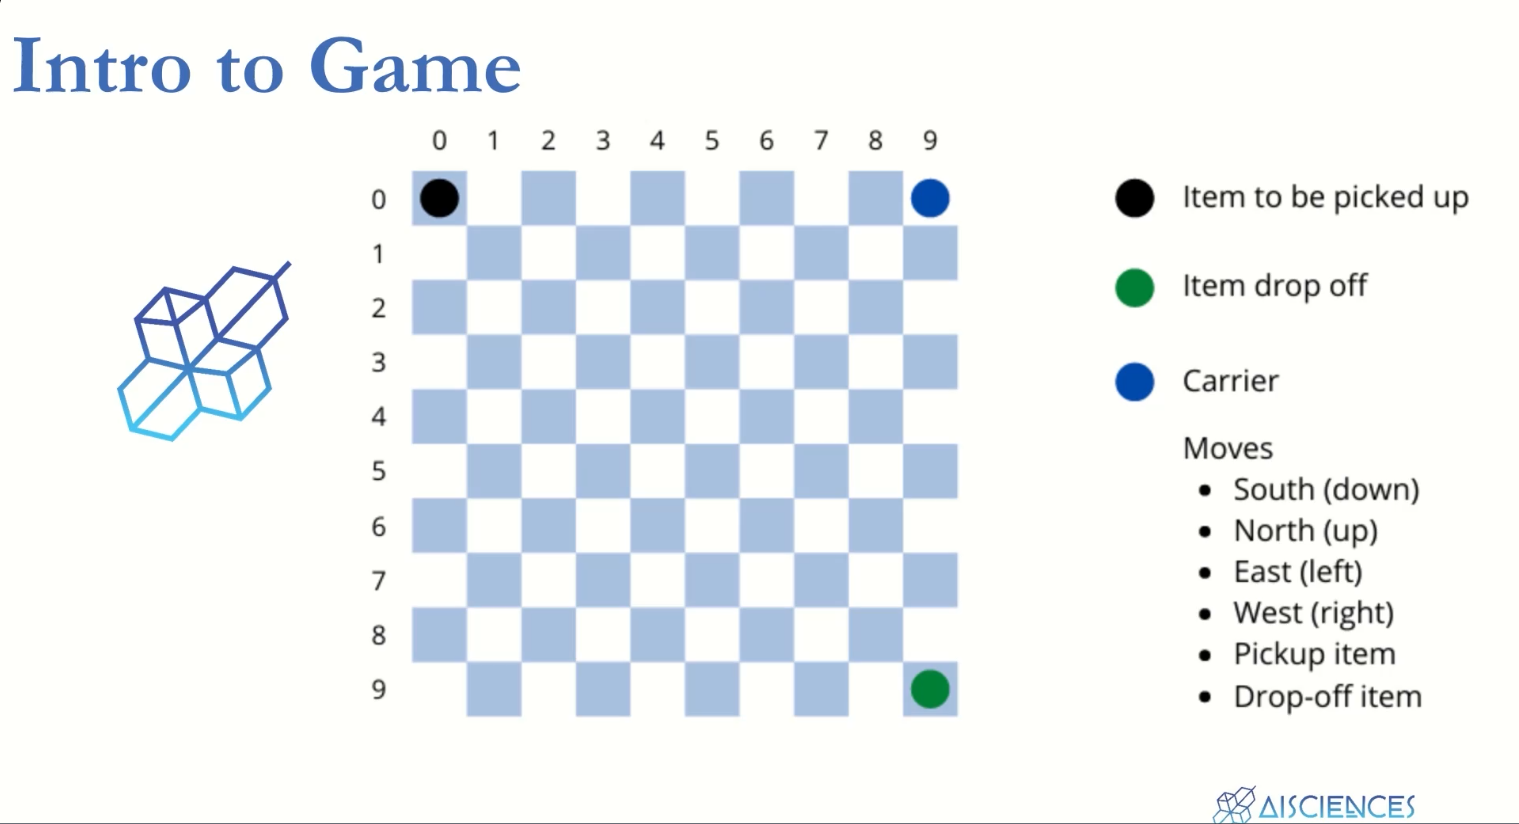
\includegraphics{assets/ch_03/drop_game.png}

}

\caption{Pick and Drop game}

\end{figure}%

}

\caption{\label{fig-pick_and_drop_exm}Pick and Drop game. See python
implementation below.}

\end{figure*}%

\begin{figure*}

\centering{

\begin{figure}[H]

{\centering 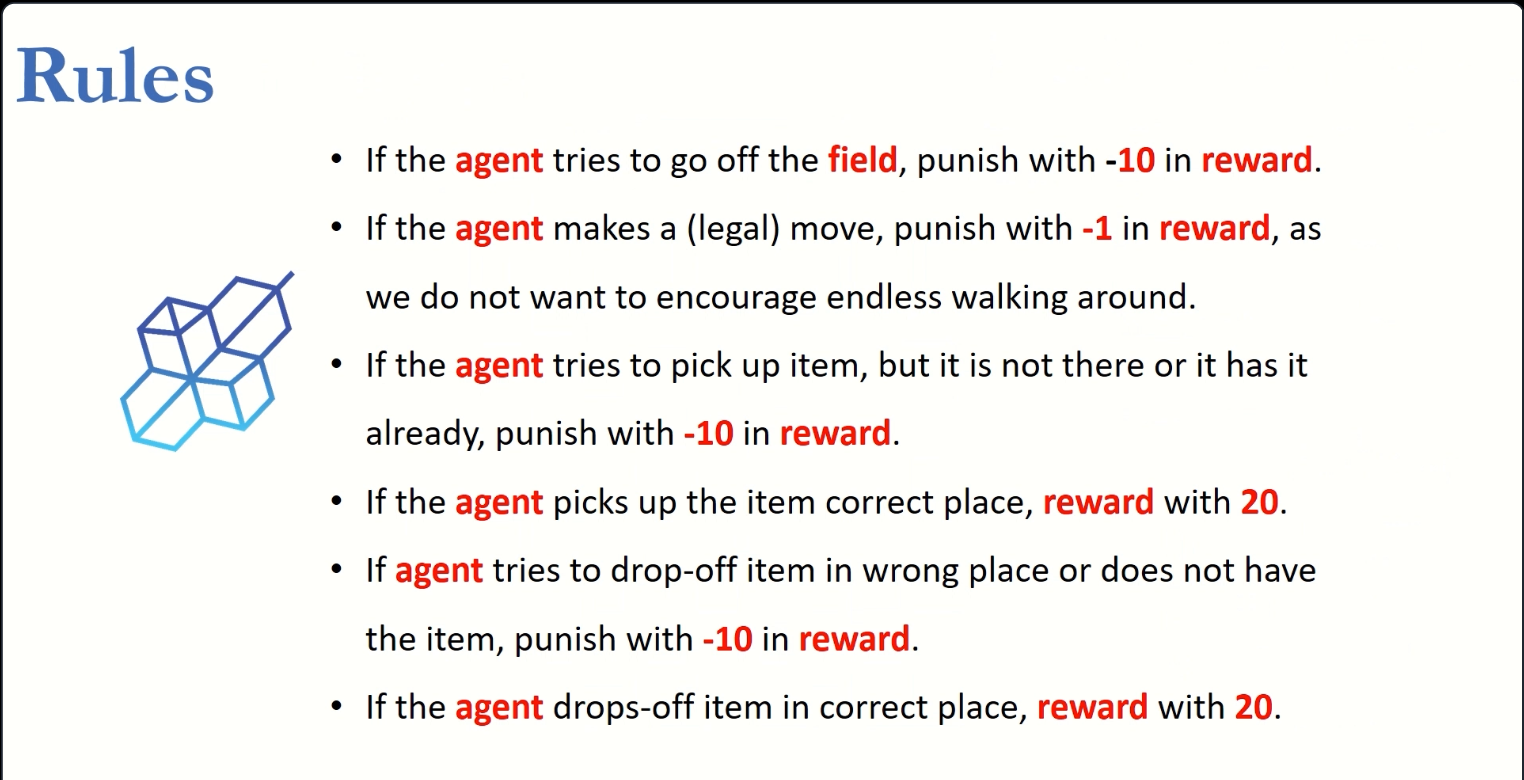
\includegraphics{assets/ch_03/rules_drop_game.png}

}

\caption{Rewards rules for the drop game}

\end{figure}%

}

\caption{\label{fig-pick_and_drop_rules}Rewards rules for the drop game.
See the above scheme for reference.}

\end{figure*}%

\begin{tcolorbox}[enhanced jigsaw, bottomrule=.15mm, opacityback=0, breakable, colframe=quarto-callout-tip-color-frame, left=2mm, rightrule=.15mm, toprule=.15mm, leftrule=.75mm, arc=.35mm, colback=white]

\vspace{-3mm}\textbf{We use the following class to simulate the pick and drop game
accordingly the}\vspace{3mm}

above figure and rules.

\begin{codelisting}[H]

\caption{\texttt{pick\_and\_drop\_game.py}}

\begin{Shaded}
\begin{Highlighting}[]
\KeywordTok{class}\NormalTok{ Field:}
    \KeywordTok{def} \FunctionTok{\_\_init\_\_}\NormalTok{(}\VariableTok{self}\NormalTok{, size, item\_pickup, item\_dropout, start\_position):}
        \VariableTok{self}\NormalTok{.size }\OperatorTok{=}\NormalTok{ size}
        \VariableTok{self}\NormalTok{.item\_pickup }\OperatorTok{=}\NormalTok{ item\_pickup}
        \VariableTok{self}\NormalTok{.item\_dropout }\OperatorTok{=}\NormalTok{ item\_dropout}
        \VariableTok{self}\NormalTok{.position }\OperatorTok{=}\NormalTok{ start\_position}
        \VariableTok{self}\NormalTok{.item\_in\_car }\OperatorTok{=} \VariableTok{False}
    
    \KeywordTok{def}\NormalTok{ get\_number\_of\_states(}\VariableTok{self}\NormalTok{):}
        \ControlFlowTok{return} \VariableTok{self}\NormalTok{.size }\OperatorTok{*} \VariableTok{self}\NormalTok{.size }\OperatorTok{*} \VariableTok{self}\NormalTok{.size }\OperatorTok{*} \VariableTok{self}\NormalTok{.size }\OperatorTok{*} \DecValTok{2}
    
    \KeywordTok{def}\NormalTok{ get\_state(}\VariableTok{self}\NormalTok{):}
\NormalTok{        state }\OperatorTok{=} \VariableTok{self}\NormalTok{.position[}\DecValTok{0}\NormalTok{] }\OperatorTok{*} \VariableTok{self}\NormalTok{.size }\OperatorTok{*} \VariableTok{self}\NormalTok{.size }\OperatorTok{*} \VariableTok{self}\NormalTok{.size }\OperatorTok{*} \DecValTok{2}
\NormalTok{        state }\OperatorTok{=}\NormalTok{ state }\OperatorTok{+} \VariableTok{self}\NormalTok{.position[}\DecValTok{1}\NormalTok{] }\OperatorTok{*} \VariableTok{self}\NormalTok{.size }\OperatorTok{*} \VariableTok{self}\NormalTok{.size }\OperatorTok{*} \DecValTok{2}
\NormalTok{        state }\OperatorTok{=}\NormalTok{ state }\OperatorTok{+} \VariableTok{self}\NormalTok{.item\_pickup[}\DecValTok{0}\NormalTok{] }\OperatorTok{*} \VariableTok{self}\NormalTok{.size }\OperatorTok{*} \DecValTok{2}
\NormalTok{        state }\OperatorTok{=}\NormalTok{ state }\OperatorTok{+} \VariableTok{self}\NormalTok{.item\_pickup[}\DecValTok{1}\NormalTok{] }\OperatorTok{*} \DecValTok{2}
        
        \ControlFlowTok{if} \VariableTok{self}\NormalTok{.item\_in\_car:}
\NormalTok{            state }\OperatorTok{=}\NormalTok{ state }\OperatorTok{+} \DecValTok{1}
        \ControlFlowTok{return}\NormalTok{ state}
    
    \KeywordTok{def}\NormalTok{ make\_action(}\VariableTok{self}\NormalTok{, action):}
\NormalTok{        (x, y) }\OperatorTok{=} \VariableTok{self}\NormalTok{.position}
        \ControlFlowTok{if}\NormalTok{ action }\OperatorTok{==} \DecValTok{0}\NormalTok{:  }\CommentTok{\# down}
            \ControlFlowTok{if}\NormalTok{ y }\OperatorTok{==} \VariableTok{self}\NormalTok{.size }\OperatorTok{{-}} \DecValTok{1}\NormalTok{:}
                \ControlFlowTok{return} \OperatorTok{{-}}\DecValTok{10}\NormalTok{, }\VariableTok{False}
            \ControlFlowTok{else}\NormalTok{:}
                \VariableTok{self}\NormalTok{.position }\OperatorTok{=}\NormalTok{ (x, y }\OperatorTok{+} \DecValTok{1}\NormalTok{)}
                \ControlFlowTok{return} \OperatorTok{{-}}\DecValTok{1}\NormalTok{, }\VariableTok{False}
        
        \ControlFlowTok{elif}\NormalTok{ action }\OperatorTok{==} \DecValTok{1}\NormalTok{:  }\CommentTok{\# up}
            \ControlFlowTok{if}\NormalTok{ y }\OperatorTok{==} \DecValTok{0}\NormalTok{:}
                \ControlFlowTok{return} \OperatorTok{{-}}\DecValTok{10}\NormalTok{, }\VariableTok{False}
            \ControlFlowTok{else}\NormalTok{:}
                \VariableTok{self}\NormalTok{.position }\OperatorTok{=}\NormalTok{ (x, y }\OperatorTok{{-}} \DecValTok{1}\NormalTok{)}
                \ControlFlowTok{return} \OperatorTok{{-}}\DecValTok{1}\NormalTok{, }\VariableTok{False}
        
        \ControlFlowTok{elif}\NormalTok{ action }\OperatorTok{==} \DecValTok{2}\NormalTok{:  }\CommentTok{\# left}
            \ControlFlowTok{if}\NormalTok{ x }\OperatorTok{==} \DecValTok{0}\NormalTok{:}
                \ControlFlowTok{return} \OperatorTok{{-}}\DecValTok{10}\NormalTok{, }\VariableTok{False}
            \ControlFlowTok{else}\NormalTok{:}
                \VariableTok{self}\NormalTok{.position }\OperatorTok{=}\NormalTok{ (x }\OperatorTok{{-}} \DecValTok{1}\NormalTok{, y)}
                \ControlFlowTok{return} \OperatorTok{{-}}\DecValTok{1}\NormalTok{, }\VariableTok{False}
        
        \ControlFlowTok{elif}\NormalTok{ action }\OperatorTok{==} \DecValTok{3}\NormalTok{:  }\CommentTok{\# right}
            \ControlFlowTok{if}\NormalTok{ x }\OperatorTok{==} \VariableTok{self}\NormalTok{.size }\OperatorTok{{-}} \DecValTok{1}\NormalTok{:}
                \ControlFlowTok{return} \OperatorTok{{-}}\DecValTok{10}\NormalTok{, }\VariableTok{False}
            \ControlFlowTok{else}\NormalTok{:}
                \VariableTok{self}\NormalTok{.position }\OperatorTok{=}\NormalTok{ (x }\OperatorTok{+} \DecValTok{1}\NormalTok{, y)}
                \ControlFlowTok{return} \OperatorTok{{-}}\DecValTok{1}\NormalTok{, }\VariableTok{False}
        
        \ControlFlowTok{elif}\NormalTok{ action }\OperatorTok{==} \DecValTok{4}\NormalTok{:  }\CommentTok{\# pickup}
            \ControlFlowTok{if} \VariableTok{self}\NormalTok{.item\_in\_car:}
                \ControlFlowTok{return} \OperatorTok{{-}}\DecValTok{10}\NormalTok{, }\VariableTok{False}
            \ControlFlowTok{elif} \VariableTok{self}\NormalTok{.item\_pickup }\OperatorTok{!=}\NormalTok{ (x, y):}
                \ControlFlowTok{return} \OperatorTok{{-}}\DecValTok{10}\NormalTok{, }\VariableTok{False}
            \ControlFlowTok{else}\NormalTok{:}
                \VariableTok{self}\NormalTok{.item\_in\_car }\OperatorTok{=} \VariableTok{True}
                \ControlFlowTok{return} \DecValTok{20}\NormalTok{, }\VariableTok{False}
        
        \ControlFlowTok{elif}\NormalTok{ action }\OperatorTok{==} \DecValTok{5}\NormalTok{:  }\CommentTok{\# dropout}
            \ControlFlowTok{if} \KeywordTok{not} \VariableTok{self}\NormalTok{.item\_in\_car:}
                \ControlFlowTok{return} \OperatorTok{{-}}\DecValTok{10}\NormalTok{, }\VariableTok{False}
            \ControlFlowTok{elif} \VariableTok{self}\NormalTok{.item\_dropout }\OperatorTok{!=}\NormalTok{ (x, y):}
                \VariableTok{self}\NormalTok{.item\_pickup }\OperatorTok{=}\NormalTok{ (x, y)}
                \VariableTok{self}\NormalTok{.item\_in\_car }\OperatorTok{=} \VariableTok{False}
                \ControlFlowTok{return} \OperatorTok{{-}}\DecValTok{10}\NormalTok{, }\VariableTok{False}
            \ControlFlowTok{else}\NormalTok{:}
                \VariableTok{self}\NormalTok{.item\_in\_car }\OperatorTok{=} \VariableTok{False}
                \ControlFlowTok{return} \DecValTok{20}\NormalTok{, }\VariableTok{True}
\end{Highlighting}
\end{Shaded}

\end{codelisting}

\end{tcolorbox}

\begin{tcolorbox}[enhanced jigsaw, bottomrule=.15mm, opacityback=0, breakable, colframe=quarto-callout-tip-color-frame, left=2mm, rightrule=.15mm, toprule=.15mm, leftrule=.75mm, arc=.35mm, colback=white]

\vspace{-3mm}\textbf{To illustrate how works this class}\vspace{3mm}

\begin{codelisting}[H]

\caption{\texttt{test\_pick\_and\_drop\_game.py}}

\begin{Shaded}
\begin{Highlighting}[]
\ImportTok{from}\NormalTok{ pick\_and\_drop\_game }\ImportTok{import}\NormalTok{ Field}
\NormalTok{size }\OperatorTok{=} \DecValTok{10}
\NormalTok{item\_pickup }\OperatorTok{=}\NormalTok{ (}\DecValTok{0}\NormalTok{, }\DecValTok{0}\NormalTok{)}
\NormalTok{item\_dropout }\OperatorTok{=}\NormalTok{ (}\DecValTok{9}\NormalTok{, }\DecValTok{9}\NormalTok{)}
\NormalTok{start\_position }\OperatorTok{=}\NormalTok{ (}\DecValTok{9}\NormalTok{, }\DecValTok{0}\NormalTok{)}



\ControlFlowTok{if} \VariableTok{\_\_name\_\_} \OperatorTok{==} \StringTok{\textquotesingle{}\_\_main\_\_\textquotesingle{}}\NormalTok{:}
\NormalTok{    field }\OperatorTok{=}\NormalTok{ Field(size, item\_pickup, item\_dropout, start\_position)}
    \BuiltInTok{print}\NormalTok{(field.position)}
    
\CommentTok{\# manual solution}
\NormalTok{field.make\_action(}\DecValTok{2}\NormalTok{)}
\NormalTok{field.make\_action(}\DecValTok{2}\NormalTok{)}
\NormalTok{field.make\_action(}\DecValTok{2}\NormalTok{)}
\NormalTok{field.make\_action(}\DecValTok{2}\NormalTok{)}
\NormalTok{field.make\_action(}\DecValTok{2}\NormalTok{)}
\NormalTok{field.make\_action(}\DecValTok{2}\NormalTok{)}
\NormalTok{field.make\_action(}\DecValTok{2}\NormalTok{)}
\NormalTok{field.make\_action(}\DecValTok{2}\NormalTok{)}
\NormalTok{field.make\_action(}\DecValTok{2}\NormalTok{)}
\CommentTok{\# pick}
\NormalTok{field.make\_action(}\DecValTok{4}\NormalTok{)}

\NormalTok{field.make\_action(}\DecValTok{0}\NormalTok{)}
\NormalTok{field.make\_action(}\DecValTok{0}\NormalTok{)}
\NormalTok{field.make\_action(}\DecValTok{0}\NormalTok{)}
\NormalTok{field.make\_action(}\DecValTok{0}\NormalTok{)}
\NormalTok{field.make\_action(}\DecValTok{0}\NormalTok{)}
\NormalTok{field.make\_action(}\DecValTok{0}\NormalTok{)}
\NormalTok{field.make\_action(}\DecValTok{0}\NormalTok{)}
\NormalTok{field.make\_action(}\DecValTok{0}\NormalTok{)}
\NormalTok{field.make\_action(}\DecValTok{0}\NormalTok{)}

\NormalTok{field.make\_action(}\DecValTok{3}\NormalTok{)}
\NormalTok{field.make\_action(}\DecValTok{3}\NormalTok{)}
\NormalTok{field.make\_action(}\DecValTok{3}\NormalTok{)}
\NormalTok{field.make\_action(}\DecValTok{3}\NormalTok{)}
\NormalTok{field.make\_action(}\DecValTok{3}\NormalTok{)}
\NormalTok{field.make\_action(}\DecValTok{3}\NormalTok{)}
\NormalTok{field.make\_action(}\DecValTok{3}\NormalTok{)}
\NormalTok{field.make\_action(}\DecValTok{3}\NormalTok{)}
\NormalTok{field.make\_action(}\DecValTok{3}\NormalTok{)}

\NormalTok{field.make\_action(}\DecValTok{5}\NormalTok{)}
\end{Highlighting}
\end{Shaded}

\end{codelisting}

\end{tcolorbox}

\begin{tcolorbox}[enhanced jigsaw, bottomrule=.15mm, opacityback=0, breakable, colframe=quarto-callout-tip-color-frame, left=2mm, rightrule=.15mm, toprule=.15mm, leftrule=.75mm, arc=.35mm, colback=white]

\vspace{-3mm}\textbf{Now we implement a random but naive solution}\vspace{3mm}

\begin{codelisting}[H]

\caption{\texttt{pick\_and\_drop\_naive\_random\_solution.py}}

\begin{Shaded}
\begin{Highlighting}[]
\ImportTok{from}\NormalTok{ matplotlib }\ImportTok{import}\NormalTok{ pyplot }\ImportTok{as}\NormalTok{ plt}

\ImportTok{from}\NormalTok{ pick\_and\_drop\_game }\ImportTok{import}\NormalTok{ Field}
\ImportTok{import}\NormalTok{ random}
\ImportTok{import}\NormalTok{ numpy }\ImportTok{as}\NormalTok{ np}


\KeywordTok{def}\NormalTok{ random\_solution():}
\NormalTok{    size }\OperatorTok{=} \DecValTok{10}
\NormalTok{    item\_pickup }\OperatorTok{=}\NormalTok{ (}\DecValTok{0}\NormalTok{, }\DecValTok{0}\NormalTok{)}
\NormalTok{    item\_dropout }\OperatorTok{=}\NormalTok{ (}\DecValTok{9}\NormalTok{, }\DecValTok{9}\NormalTok{)}
\NormalTok{    start\_position }\OperatorTok{=}\NormalTok{ (}\DecValTok{9}\NormalTok{, }\DecValTok{0}\NormalTok{)}
    
\NormalTok{    field }\OperatorTok{=}\NormalTok{ Field(size, item\_pickup, item\_dropout, start\_position)}
    
\NormalTok{    done }\OperatorTok{=} \VariableTok{False}
\NormalTok{    steps }\OperatorTok{=} \DecValTok{0}
    
    \ControlFlowTok{while} \KeywordTok{not}\NormalTok{ done:}
\NormalTok{        action }\OperatorTok{=}\NormalTok{ random.randint(}\DecValTok{0}\NormalTok{, }\DecValTok{5}\NormalTok{)}
\NormalTok{        reward, done }\OperatorTok{=}\NormalTok{ field.make\_action(action)}
\NormalTok{        steps }\OperatorTok{=}\NormalTok{ steps }\OperatorTok{+} \DecValTok{1}
    
    \ControlFlowTok{return}\NormalTok{ steps}


\ControlFlowTok{if} \VariableTok{\_\_name\_\_} \OperatorTok{==} \StringTok{\textquotesingle{}\_\_main\_\_\textquotesingle{}}\NormalTok{:}
\NormalTok{    steps }\OperatorTok{=}\NormalTok{ random\_solution()}
    \BuiltInTok{print}\NormalTok{(steps)}
\NormalTok{    sampling\_size }\OperatorTok{=} \DecValTok{100}
\NormalTok{    sample }\OperatorTok{=}\NormalTok{ [random\_solution() }\ControlFlowTok{for}\NormalTok{ \_ }\KeywordTok{in} \BuiltInTok{range}\NormalTok{(sampling\_size)]}
\NormalTok{    sample }\OperatorTok{=}\NormalTok{ np.array(sample)}
\NormalTok{    no\_steps\_mean }\OperatorTok{=}\NormalTok{ sample.mean()}
    \BuiltInTok{print}\NormalTok{(}\StringTok{\textquotesingle{}Mean of \# steps for reach goal }\SpecialCharTok{\{:n\}}\StringTok{\textquotesingle{}}\NormalTok{.}\BuiltInTok{format}\NormalTok{(no\_steps\_mean))}
\NormalTok{    plt.show()}
\end{Highlighting}
\end{Shaded}

\end{codelisting}

\end{tcolorbox}

\begin{tcolorbox}[enhanced jigsaw, bottomrule=.15mm, opacityback=0, breakable, colframe=quarto-callout-tip-color-frame, left=2mm, rightrule=.15mm, toprule=.15mm, leftrule=.75mm, arc=.35mm, colback=white]

\vspace{-3mm}\textbf{Next we apply the \(Q-\)learning algorithm for impove the above
solution.}\vspace{3mm}

\begin{codelisting}[H]

\caption{\texttt{pick\_and\_drop\_q\_learning\_solution.py}}

\begin{Shaded}
\begin{Highlighting}[]
    \KeywordTok{def}\NormalTok{ q\_learning\_solution():}
\NormalTok{    epsilon }\OperatorTok{=} \FloatTok{0.1}
\NormalTok{    alpha }\OperatorTok{=} \FloatTok{0.1}
\NormalTok{    gamma }\OperatorTok{=} \FloatTok{0.6}
    
\NormalTok{    field }\OperatorTok{=}\NormalTok{ Field(size, item\_pickup, item\_drop\_out, start\_position)}
\NormalTok{    done }\OperatorTok{=} \VariableTok{False}
\NormalTok{    steps }\OperatorTok{=} \DecValTok{0}
    
    \ControlFlowTok{while} \KeywordTok{not}\NormalTok{ done:}
\NormalTok{        state }\OperatorTok{=}\NormalTok{ field.get\_state()}
        \ControlFlowTok{if}\NormalTok{ random.uniform(}\DecValTok{0}\NormalTok{, }\DecValTok{1}\NormalTok{) }\OperatorTok{\textless{}}\NormalTok{ epsilon:}
\NormalTok{            action }\OperatorTok{=}\NormalTok{ random.randint(}\DecValTok{0}\NormalTok{, }\DecValTok{5}\NormalTok{)  }\CommentTok{\# Explore}
        \ControlFlowTok{else}\NormalTok{:}
\NormalTok{            action }\OperatorTok{=}\NormalTok{ np.argmax(q\_table[state])  }\CommentTok{\# Exploit}
        
\NormalTok{        reward, done }\OperatorTok{=}\NormalTok{ field.make\_action(action)}
        
\NormalTok{        new\_state }\OperatorTok{=}\NormalTok{ field.get\_state()}
\NormalTok{        new\_state\_max }\OperatorTok{=}\NormalTok{ np.}\BuiltInTok{max}\NormalTok{(q\_table[new\_state])}
        
\NormalTok{        q\_table[state, action] }\OperatorTok{=} \OperatorTok{\textbackslash{}}
\NormalTok{            (}\DecValTok{1} \OperatorTok{{-}}\NormalTok{ alpha) }\OperatorTok{*}\NormalTok{ q\_table[state, action] }\OperatorTok{\textbackslash{}}
            \OperatorTok{+}\NormalTok{ alpha }\OperatorTok{*}\NormalTok{ (}
\NormalTok{                    reward }\OperatorTok{+}\NormalTok{ gamma }\OperatorTok{*}\NormalTok{ new\_state\_max}
                    \OperatorTok{{-}}\NormalTok{ q\_table[state, action]}
\NormalTok{            )}
\NormalTok{        steps }\OperatorTok{=}\NormalTok{ steps }\OperatorTok{+} \DecValTok{1}
    \ControlFlowTok{return}\NormalTok{ steps}


\NormalTok{size }\OperatorTok{=} \DecValTok{10}
\NormalTok{item\_pickup }\OperatorTok{=}\NormalTok{ (}\DecValTok{0}\NormalTok{, }\DecValTok{0}\NormalTok{)}
\NormalTok{item\_drop\_out }\OperatorTok{=}\NormalTok{ (}\DecValTok{9}\NormalTok{, }\DecValTok{9}\NormalTok{)}
\NormalTok{start\_position }\OperatorTok{=}\NormalTok{ (}\DecValTok{9}\NormalTok{, }\DecValTok{0}\NormalTok{)}

\NormalTok{field }\OperatorTok{=}\NormalTok{ Field(size, item\_pickup, item\_drop\_out, start\_position)}

\NormalTok{number\_of\_states }\OperatorTok{=}\NormalTok{ field.get\_number\_of\_states()}
\NormalTok{number\_of\_actions }\OperatorTok{=} \DecValTok{6}
\NormalTok{q\_table }\OperatorTok{=}\NormalTok{ np.zeros((number\_of\_states, number\_of\_actions))}
\NormalTok{epsilon }\OperatorTok{=} \FloatTok{0.1}
\NormalTok{alpha }\OperatorTok{=} \FloatTok{0.1}
\NormalTok{gamma }\OperatorTok{=} \FloatTok{0.6}
\NormalTok{n\_training }\OperatorTok{=} \DecValTok{100000}
\CommentTok{\# Training phase}

\ControlFlowTok{for}\NormalTok{ \_ }\KeywordTok{in} \BuiltInTok{range}\NormalTok{(n\_training):}
\NormalTok{    field }\OperatorTok{=}\NormalTok{ Field(size, item\_pickup, item\_drop\_out, start\_position)}
\NormalTok{    done }\OperatorTok{=} \VariableTok{False}
    \ControlFlowTok{while} \KeywordTok{not}\NormalTok{ done:}
\NormalTok{        state }\OperatorTok{=}\NormalTok{ field.get\_state()}
        \ControlFlowTok{if}\NormalTok{ random.uniform(}\DecValTok{0}\NormalTok{, }\DecValTok{1}\NormalTok{) }\OperatorTok{\textless{}}\NormalTok{ epsilon:}
\NormalTok{            action }\OperatorTok{=}\NormalTok{ random.randint(}\DecValTok{0}\NormalTok{, }\DecValTok{5}\NormalTok{)  }\CommentTok{\# Explore}
        \ControlFlowTok{else}\NormalTok{:}
\NormalTok{            action }\OperatorTok{=}\NormalTok{ np.argmax(q\_table[state])  }\CommentTok{\# Exploit}
\NormalTok{        reward, done }\OperatorTok{=}\NormalTok{ field.make\_action(action)}
\NormalTok{        new\_state }\OperatorTok{=}\NormalTok{ field.get\_state()}
\NormalTok{        new\_state\_max }\OperatorTok{=}\NormalTok{ np.}\BuiltInTok{max}\NormalTok{(q\_table[new\_state])}
        \CommentTok{\# q\_learning iteration as ascendant grad}
\NormalTok{        q\_table[state, action] }\OperatorTok{=} \OperatorTok{\textbackslash{}}
\NormalTok{            (}\FloatTok{1.0} \OperatorTok{{-}}\NormalTok{ alpha) }\OperatorTok{*}\NormalTok{ q\_table[state, action] }\OperatorTok{\textbackslash{}}
            \OperatorTok{+}\NormalTok{ alpha }\OperatorTok{*}\NormalTok{ (}
\NormalTok{                reward }\OperatorTok{+}\NormalTok{ gamma }\OperatorTok{*}\NormalTok{ new\_state\_max }\OperatorTok{{-}}\NormalTok{ q\_table[state, action]}
\NormalTok{            )}

\NormalTok{q\_learning\_sampling }\OperatorTok{=}\NormalTok{ [q\_learning\_solution() }\ControlFlowTok{for}\NormalTok{ \_ }\KeywordTok{in} \BuiltInTok{range}\NormalTok{(}\DecValTok{10000}\NormalTok{)]}
\NormalTok{fig, ax }\OperatorTok{=}\NormalTok{ plt.subplots()}
\NormalTok{ax.hist(q\_learning\_sampling, bins}\OperatorTok{=}\DecValTok{100}\NormalTok{)}
\NormalTok{ax.set\_title(}\StringTok{\textquotesingle{}distribution of the No. of steps with the Q{-}Learning sol\textquotesingle{}}\NormalTok{)}
\NormalTok{ax.set\_xlabel(}\StringTok{\textquotesingle{}No. of steps\textquotesingle{}}\NormalTok{)}
\NormalTok{ax.set\_ylabel(}\StringTok{\textquotesingle{}Count\textquotesingle{}}\NormalTok{)}
\NormalTok{fig.savefig(}\StringTok{"histogram\_q\_learning\_solution.png"}\NormalTok{)}
\NormalTok{plt.show()}
\end{Highlighting}
\end{Shaded}

\end{codelisting}

\end{tcolorbox}

\begin{example}[Gridworld]\protect\hypertarget{exm-grid_world}{}\label{exm-grid_world}

~

\begin{itemize}
\item
  Actions: \texttt{north}, \texttt{south}, \texttt{east}, \texttt{west}
\item
  Rewards:

  \begin{itemize}
  \tightlist
  \item
    Actions would take the agent off the grid leave its location
    unchanged, but also results in a reward of-1;
  \item
    Other actions result in a reward of 0, except those that in states A
    and B;
  \item
    From state A , all four actions yield a reward of +10 and take the
    agent toA' ;
  \item
    From state B , all four actions yield a reward of +5 and take the
    agentto B' ;
  \item
    The learning rate (\(\gamma\)) for this example is 0.9
  \end{itemize}
\end{itemize}

\begin{figure*}

\centering{

\begin{figure}[H]

{\centering 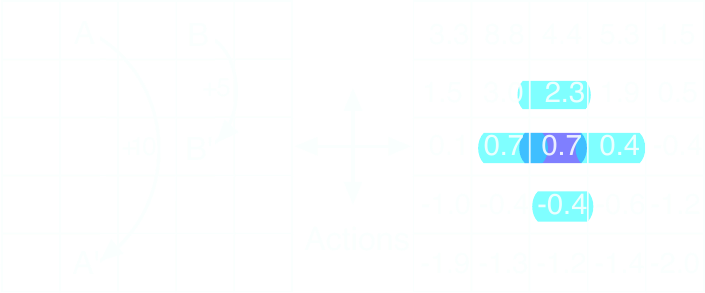
\includegraphics{assets/ch_04/grid_world_exm.png}

}

\caption{Grid World example. Problem scheme , possible actions and
sampling reward}

\end{figure}%

}

\caption{\label{fig-grid-world-exm}Grid World example. Problem scheme ,
possible actions and sampling reward}

\end{figure*}%

The Bellman equation must hold for each state for the value function
\(v_{\pi}\) shown in Figure~\ref{fig-grid-world-exm} (right). Show
numerically that this equation holds for the center state, valued at
+0.7, with respect to its four neighboring states, valued at +2.3, +0.4,
0.4, and +0.7. (These numbers are accurate only to one decimal place.)

\begin{tcolorbox}[enhanced jigsaw, bottomrule=.15mm, opacityback=0, breakable, colframe=quarto-callout-tip-color-frame, left=2mm, rightrule=.15mm, toprule=.15mm, leftrule=.75mm, arc=.35mm, colback=white]

\vspace{-3mm}\textbf{python implementation for the grid-world example}\vspace{3mm}

\begin{codelisting}[H]

\caption{\texttt{gridworld.py}}

\begin{Shaded}
\begin{Highlighting}[]
\CommentTok{\#| lst{-}label: lst{-}import}
\CommentTok{\#| lst{-}cap: Import pyplot}
\ImportTok{import}\NormalTok{ matplotlib}
\ImportTok{import}\NormalTok{ matplotlib.pyplot }\ImportTok{as}\NormalTok{ plt}
\ImportTok{import}\NormalTok{ numpy }\ImportTok{as}\NormalTok{ np}
\ImportTok{from}\NormalTok{ matplotlib.table }\ImportTok{import}\NormalTok{ Table}
\NormalTok{matplotlib.use(}\StringTok{\textquotesingle{}Agg\textquotesingle{}}\NormalTok{)}

\NormalTok{WORLD\_SIZE }\OperatorTok{=} \DecValTok{5}
\NormalTok{A\_POS }\OperatorTok{=}\NormalTok{ [}\DecValTok{0}\NormalTok{, }\DecValTok{1}\NormalTok{]}
\NormalTok{A\_PRIME\_POS }\OperatorTok{=}\NormalTok{ [}\DecValTok{4}\NormalTok{, }\DecValTok{1}\NormalTok{]}
\NormalTok{B\_POS }\OperatorTok{=}\NormalTok{ [}\DecValTok{0}\NormalTok{, }\DecValTok{3}\NormalTok{]}
\NormalTok{B\_PRIME\_POS }\OperatorTok{=}\NormalTok{ [}\DecValTok{2}\NormalTok{, }\DecValTok{3}\NormalTok{]}
\NormalTok{DISCOUNT }\OperatorTok{=} \FloatTok{0.9}

\CommentTok{\# left, up, right, down}
\NormalTok{ACTIONS }\OperatorTok{=}\NormalTok{ [np.array([}\DecValTok{0}\NormalTok{, }\OperatorTok{{-}}\DecValTok{1}\NormalTok{]),}
\NormalTok{           np.array([}\OperatorTok{{-}}\DecValTok{1}\NormalTok{, }\DecValTok{0}\NormalTok{]),}
\NormalTok{           np.array([}\DecValTok{0}\NormalTok{, }\DecValTok{1}\NormalTok{]),}
\NormalTok{           np.array([}\DecValTok{1}\NormalTok{, }\DecValTok{0}\NormalTok{])]}
\NormalTok{ACTIONS\_FIGS }\OperatorTok{=}\NormalTok{ [}\StringTok{\textquotesingle{}←\textquotesingle{}}\NormalTok{, }\StringTok{\textquotesingle{}↑\textquotesingle{}}\NormalTok{, }\StringTok{\textquotesingle{}→\textquotesingle{}}\NormalTok{, }\StringTok{\textquotesingle{}↓\textquotesingle{}}\NormalTok{]}
\NormalTok{ACTION\_PROB }\OperatorTok{=} \FloatTok{0.25}

\KeywordTok{def}\NormalTok{ step(state, action):}
    \ControlFlowTok{if}\NormalTok{ state }\OperatorTok{==}\NormalTok{ A\_POS:}
        \ControlFlowTok{return}\NormalTok{ A\_PRIME\_POS, }\DecValTok{10}
    \ControlFlowTok{if}\NormalTok{ state }\OperatorTok{==}\NormalTok{ B\_POS:}
        \ControlFlowTok{return}\NormalTok{ B\_PRIME\_POS, }\DecValTok{5}

\NormalTok{    next\_state }\OperatorTok{=}\NormalTok{ (np.array(state) }\OperatorTok{+}\NormalTok{ action).tolist()}
\NormalTok{    x, y }\OperatorTok{=}\NormalTok{ next\_state}
    \ControlFlowTok{if}\NormalTok{ x }\OperatorTok{\textless{}} \DecValTok{0} \KeywordTok{or}\NormalTok{ x }\OperatorTok{\textgreater{}=}\NormalTok{ WORLD\_SIZE }\KeywordTok{or}\NormalTok{ y }\OperatorTok{\textless{}} \DecValTok{0} \KeywordTok{or}\NormalTok{ y }\OperatorTok{\textgreater{}=}\NormalTok{ WORLD\_SIZE:}
\NormalTok{        reward }\OperatorTok{=} \OperatorTok{{-}}\FloatTok{1.0}
\NormalTok{        next\_state }\OperatorTok{=}\NormalTok{ state}
    \ControlFlowTok{else}\NormalTok{:}
\NormalTok{        reward }\OperatorTok{=} \DecValTok{0}
    \ControlFlowTok{return}\NormalTok{ next\_state, reward}


\KeywordTok{def}\NormalTok{ draw\_image(image):}
\NormalTok{    fig, ax }\OperatorTok{=}\NormalTok{ plt.subplots()}
\NormalTok{    ax.set\_axis\_off()}
\NormalTok{    tb }\OperatorTok{=}\NormalTok{ Table(ax, bbox}\OperatorTok{=}\NormalTok{[}\DecValTok{0}\NormalTok{, }\DecValTok{0}\NormalTok{, }\DecValTok{1}\NormalTok{, }\DecValTok{1}\NormalTok{])}

\NormalTok{    nrows, ncols }\OperatorTok{=}\NormalTok{ image.shape}
\NormalTok{    width, height }\OperatorTok{=} \FloatTok{1.0} \OperatorTok{/}\NormalTok{ ncols, }\FloatTok{1.0} \OperatorTok{/}\NormalTok{ nrows}

    \CommentTok{\# Add cells}
    \ControlFlowTok{for}\NormalTok{ (i, j), val }\KeywordTok{in}\NormalTok{ np.ndenumerate(image):}

        \CommentTok{\# add state labels}
        \ControlFlowTok{if}\NormalTok{ [i, j] }\OperatorTok{==}\NormalTok{ A\_POS:}
\NormalTok{            val }\OperatorTok{=} \BuiltInTok{str}\NormalTok{(val) }\OperatorTok{+} \StringTok{" (A)"}
        \ControlFlowTok{if}\NormalTok{ [i, j] }\OperatorTok{==}\NormalTok{ A\_PRIME\_POS:}
\NormalTok{            val }\OperatorTok{=} \BuiltInTok{str}\NormalTok{(val) }\OperatorTok{+} \StringTok{" (A\textquotesingle{})"}
        \ControlFlowTok{if}\NormalTok{ [i, j] }\OperatorTok{==}\NormalTok{ B\_POS:}
\NormalTok{            val }\OperatorTok{=} \BuiltInTok{str}\NormalTok{(val) }\OperatorTok{+} \StringTok{" (B)"}
        \ControlFlowTok{if}\NormalTok{ [i, j] }\OperatorTok{==}\NormalTok{ B\_PRIME\_POS:}
\NormalTok{            val }\OperatorTok{=} \BuiltInTok{str}\NormalTok{(val) }\OperatorTok{+} \StringTok{" (B\textquotesingle{})"}
        
\NormalTok{        tb.add\_cell(i, j, width, height, text}\OperatorTok{=}\NormalTok{val,}
\NormalTok{                    loc}\OperatorTok{=}\StringTok{\textquotesingle{}center\textquotesingle{}}\NormalTok{, facecolor}\OperatorTok{=}\StringTok{\textquotesingle{}white\textquotesingle{}}\NormalTok{)}
        
    \CommentTok{\# Row and column labels...}
    \ControlFlowTok{for}\NormalTok{ i }\KeywordTok{in} \BuiltInTok{range}\NormalTok{(}\BuiltInTok{len}\NormalTok{(image)):}
\NormalTok{        tb.add\_cell(i, }\OperatorTok{{-}}\DecValTok{1}\NormalTok{, width, height, text}\OperatorTok{=}\NormalTok{i}\OperatorTok{+}\DecValTok{1}\NormalTok{, loc}\OperatorTok{=}\StringTok{\textquotesingle{}right\textquotesingle{}}\NormalTok{,}
\NormalTok{                    edgecolor}\OperatorTok{=}\StringTok{\textquotesingle{}none\textquotesingle{}}\NormalTok{, facecolor}\OperatorTok{=}\StringTok{\textquotesingle{}none\textquotesingle{}}\NormalTok{)}
\NormalTok{        tb.add\_cell(}\OperatorTok{{-}}\DecValTok{1}\NormalTok{, i, width, height}\OperatorTok{/}\DecValTok{2}\NormalTok{, text}\OperatorTok{=}\NormalTok{i}\OperatorTok{+}\DecValTok{1}\NormalTok{, loc}\OperatorTok{=}\StringTok{\textquotesingle{}center\textquotesingle{}}\NormalTok{,}
\NormalTok{                    edgecolor}\OperatorTok{=}\StringTok{\textquotesingle{}none\textquotesingle{}}\NormalTok{, facecolor}\OperatorTok{=}\StringTok{\textquotesingle{}none\textquotesingle{}}\NormalTok{)}

\NormalTok{    ax.add\_table(tb)}

\KeywordTok{def}\NormalTok{ draw\_policy(optimal\_values):}
\NormalTok{    fig, ax }\OperatorTok{=}\NormalTok{ plt.subplots()}
\NormalTok{    ax.set\_axis\_off()}
\NormalTok{    tb }\OperatorTok{=}\NormalTok{ Table(ax, bbox}\OperatorTok{=}\NormalTok{[}\DecValTok{0}\NormalTok{, }\DecValTok{0}\NormalTok{, }\DecValTok{1}\NormalTok{, }\DecValTok{1}\NormalTok{])}

\NormalTok{    nrows, ncols }\OperatorTok{=}\NormalTok{ optimal\_values.shape}
\NormalTok{    width, height }\OperatorTok{=} \FloatTok{1.0} \OperatorTok{/}\NormalTok{ ncols, }\FloatTok{1.0} \OperatorTok{/}\NormalTok{ nrows}

    \CommentTok{\# Add cells}
    \ControlFlowTok{for}\NormalTok{ (i, j), val }\KeywordTok{in}\NormalTok{ np.ndenumerate(optimal\_values):}
\NormalTok{        next\_vals}\OperatorTok{=}\NormalTok{[]}
        \ControlFlowTok{for}\NormalTok{ action }\KeywordTok{in}\NormalTok{ ACTIONS:}
\NormalTok{            next\_state, \_ }\OperatorTok{=}\NormalTok{ step([i, j], action)}
\NormalTok{            next\_vals.append(optimal\_values[next\_state[}\DecValTok{0}\NormalTok{],next\_state[}\DecValTok{1}\NormalTok{]])}

\NormalTok{        best\_actions}\OperatorTok{=}\NormalTok{np.where(next\_vals }\OperatorTok{==}\NormalTok{ np.}\BuiltInTok{max}\NormalTok{(next\_vals))[}\DecValTok{0}\NormalTok{]}
\NormalTok{        val}\OperatorTok{=}\StringTok{\textquotesingle{}\textquotesingle{}}
        \ControlFlowTok{for}\NormalTok{ ba }\KeywordTok{in}\NormalTok{ best\_actions:}
\NormalTok{            val}\OperatorTok{+=}\NormalTok{ACTIONS\_FIGS[ba]}
        
        \CommentTok{\# add state labels}
        \ControlFlowTok{if}\NormalTok{ [i, j] }\OperatorTok{==}\NormalTok{ A\_POS:}
\NormalTok{            val }\OperatorTok{=} \BuiltInTok{str}\NormalTok{(val) }\OperatorTok{+} \StringTok{" (A)"}
        \ControlFlowTok{if}\NormalTok{ [i, j] }\OperatorTok{==}\NormalTok{ A\_PRIME\_POS:}
\NormalTok{            val }\OperatorTok{=} \BuiltInTok{str}\NormalTok{(val) }\OperatorTok{+} \StringTok{" (A\textquotesingle{})"}
        \ControlFlowTok{if}\NormalTok{ [i, j] }\OperatorTok{==}\NormalTok{ B\_POS:}
\NormalTok{            val }\OperatorTok{=} \BuiltInTok{str}\NormalTok{(val) }\OperatorTok{+} \StringTok{" (B)"}
        \ControlFlowTok{if}\NormalTok{ [i, j] }\OperatorTok{==}\NormalTok{ B\_PRIME\_POS:}
\NormalTok{            val }\OperatorTok{=} \BuiltInTok{str}\NormalTok{(val) }\OperatorTok{+} \StringTok{" (B\textquotesingle{})"}
        
\NormalTok{        tb.add\_cell(i, j, width, height, text}\OperatorTok{=}\NormalTok{val,}
\NormalTok{                loc}\OperatorTok{=}\StringTok{\textquotesingle{}center\textquotesingle{}}\NormalTok{, facecolor}\OperatorTok{=}\StringTok{\textquotesingle{}white\textquotesingle{}}\NormalTok{)}

    \CommentTok{\# Row and column labels...}
    \ControlFlowTok{for}\NormalTok{ i }\KeywordTok{in} \BuiltInTok{range}\NormalTok{(}\BuiltInTok{len}\NormalTok{(optimal\_values)):}
\NormalTok{        tb.add\_cell(i, }\OperatorTok{{-}}\DecValTok{1}\NormalTok{, width, height, text}\OperatorTok{=}\NormalTok{i}\OperatorTok{+}\DecValTok{1}\NormalTok{, loc}\OperatorTok{=}\StringTok{\textquotesingle{}right\textquotesingle{}}\NormalTok{,}
\NormalTok{                    edgecolor}\OperatorTok{=}\StringTok{\textquotesingle{}none\textquotesingle{}}\NormalTok{, facecolor}\OperatorTok{=}\StringTok{\textquotesingle{}none\textquotesingle{}}\NormalTok{)}
\NormalTok{        tb.add\_cell(}\OperatorTok{{-}}\DecValTok{1}\NormalTok{, i, width, height}\OperatorTok{/}\DecValTok{2}\NormalTok{, text}\OperatorTok{=}\NormalTok{i}\OperatorTok{+}\DecValTok{1}\NormalTok{, loc}\OperatorTok{=}\StringTok{\textquotesingle{}center\textquotesingle{}}\NormalTok{,}
\NormalTok{                   edgecolor}\OperatorTok{=}\StringTok{\textquotesingle{}none\textquotesingle{}}\NormalTok{, facecolor}\OperatorTok{=}\StringTok{\textquotesingle{}none\textquotesingle{}}\NormalTok{)}

\NormalTok{    ax.add\_table(tb)}


\KeywordTok{def}\NormalTok{ figure\_3\_2():}
\NormalTok{    value }\OperatorTok{=}\NormalTok{ np.zeros((WORLD\_SIZE, WORLD\_SIZE))}
    \ControlFlowTok{while} \VariableTok{True}\NormalTok{:}
        \CommentTok{\# keep iteration until convergence}
\NormalTok{        new\_value }\OperatorTok{=}\NormalTok{ np.zeros\_like(value)}
        \ControlFlowTok{for}\NormalTok{ i }\KeywordTok{in} \BuiltInTok{range}\NormalTok{(WORLD\_SIZE):}
            \ControlFlowTok{for}\NormalTok{ j }\KeywordTok{in} \BuiltInTok{range}\NormalTok{(WORLD\_SIZE):}
                \ControlFlowTok{for}\NormalTok{ action }\KeywordTok{in}\NormalTok{ ACTIONS:}
\NormalTok{                    (next\_i, next\_j), reward }\OperatorTok{=}\NormalTok{ step([i, j], action)}
                    \CommentTok{\# bellman equation}
\NormalTok{                    new\_value[i, j] }\OperatorTok{+=} \OperatorTok{\textbackslash{}}
\NormalTok{                        ACTION\_PROB }\OperatorTok{*}\NormalTok{ (}
\NormalTok{                                reward }\OperatorTok{+}\NormalTok{ DISCOUNT }\OperatorTok{*}\NormalTok{ value[next\_i, next\_j]}
\NormalTok{                        )}
                    
        \ControlFlowTok{if}\NormalTok{ np.}\BuiltInTok{sum}\NormalTok{(np.}\BuiltInTok{abs}\NormalTok{(value }\OperatorTok{{-}}\NormalTok{ new\_value)) }\OperatorTok{\textless{}} \FloatTok{1e{-}4}\NormalTok{:}
\NormalTok{            draw\_image(np.}\BuiltInTok{round}\NormalTok{(new\_value, decimals}\OperatorTok{=}\DecValTok{2}\NormalTok{))}
\NormalTok{            plt.savefig(}\StringTok{\textquotesingle{}../images/figure\_3\_2.png\textquotesingle{}}\NormalTok{)}
\NormalTok{            plt.close()}
            \ControlFlowTok{break}
\NormalTok{        value }\OperatorTok{=}\NormalTok{ new\_value}

\KeywordTok{def}\NormalTok{ figure\_3\_2\_linear\_system():}
    \CommentTok{\textquotesingle{}\textquotesingle{}\textquotesingle{}}
\CommentTok{    Here we solve the linear system of equations to find the exact solution.}
\CommentTok{    We do this by filling the coefficients for each of the states with their respective right side constant.}
\CommentTok{    \textquotesingle{}\textquotesingle{}\textquotesingle{}}
\NormalTok{    A }\OperatorTok{=} \OperatorTok{{-}}\DecValTok{1} \OperatorTok{*}\NormalTok{ np.eye(WORLD\_SIZE }\OperatorTok{*}\NormalTok{ WORLD\_SIZE)}
\NormalTok{    b }\OperatorTok{=}\NormalTok{ np.zeros(WORLD\_SIZE }\OperatorTok{*}\NormalTok{ WORLD\_SIZE)}
    \ControlFlowTok{for}\NormalTok{ i }\KeywordTok{in} \BuiltInTok{range}\NormalTok{(WORLD\_SIZE):}
        \ControlFlowTok{for}\NormalTok{ j }\KeywordTok{in} \BuiltInTok{range}\NormalTok{(WORLD\_SIZE):}
\NormalTok{            s }\OperatorTok{=}\NormalTok{ [i, j]  }\CommentTok{\# current state}
\NormalTok{            index\_s }\OperatorTok{=}\NormalTok{ np.ravel\_multi\_index(s, (WORLD\_SIZE, WORLD\_SIZE))}
            \ControlFlowTok{for}\NormalTok{ a }\KeywordTok{in}\NormalTok{ ACTIONS:}
\NormalTok{                s\_, r }\OperatorTok{=}\NormalTok{ step(s, a)}
\NormalTok{                index\_s\_ }\OperatorTok{=}\NormalTok{ np.ravel\_multi\_index(s\_, (WORLD\_SIZE, WORLD\_SIZE))}

\NormalTok{                A[index\_s, index\_s\_] }\OperatorTok{+=}\NormalTok{ ACTION\_PROB }\OperatorTok{*}\NormalTok{ DISCOUNT}
\NormalTok{                b[index\_s] }\OperatorTok{{-}=}\NormalTok{ ACTION\_PROB }\OperatorTok{*}\NormalTok{ r}

\NormalTok{    x }\OperatorTok{=}\NormalTok{ np.linalg.solve(A, b)}
\NormalTok{    draw\_image(np.}\BuiltInTok{round}\NormalTok{(x.reshape(WORLD\_SIZE, WORLD\_SIZE), decimals}\OperatorTok{=}\DecValTok{2}\NormalTok{))}
\NormalTok{    plt.savefig(}\StringTok{\textquotesingle{}../images/figure\_3\_2\_linear\_system.png\textquotesingle{}}\NormalTok{)}
\NormalTok{    plt.close()}

\KeywordTok{def}\NormalTok{ figure\_3\_5():}
\NormalTok{    value }\OperatorTok{=}\NormalTok{ np.zeros((WORLD\_SIZE, WORLD\_SIZE))}
    \ControlFlowTok{while} \VariableTok{True}\NormalTok{:}
        \CommentTok{\# keep iteration until convergence}
\NormalTok{        new\_value }\OperatorTok{=}\NormalTok{ np.zeros\_like(value)}
        \ControlFlowTok{for}\NormalTok{ i }\KeywordTok{in} \BuiltInTok{range}\NormalTok{(WORLD\_SIZE):}
            \ControlFlowTok{for}\NormalTok{ j }\KeywordTok{in} \BuiltInTok{range}\NormalTok{(WORLD\_SIZE):}
\NormalTok{                values }\OperatorTok{=}\NormalTok{ []}
                \ControlFlowTok{for}\NormalTok{ action }\KeywordTok{in}\NormalTok{ ACTIONS:}
\NormalTok{                    (next\_i, next\_j), reward }\OperatorTok{=}\NormalTok{ step([i, j], action)}
                    \CommentTok{\# value iteration}
\NormalTok{                    values.append(reward }\OperatorTok{+}\NormalTok{ DISCOUNT }\OperatorTok{*}\NormalTok{ value[next\_i, next\_j])}
\NormalTok{                new\_value[i, j] }\OperatorTok{=}\NormalTok{ np.}\BuiltInTok{max}\NormalTok{(values)}
        \ControlFlowTok{if}\NormalTok{ np.}\BuiltInTok{sum}\NormalTok{(np.}\BuiltInTok{abs}\NormalTok{(new\_value }\OperatorTok{{-}}\NormalTok{ value)) }\OperatorTok{\textless{}} \FloatTok{1e{-}4}\NormalTok{:}
\NormalTok{            draw\_image(np.}\BuiltInTok{round}\NormalTok{(new\_value, decimals}\OperatorTok{=}\DecValTok{2}\NormalTok{))}
\NormalTok{            plt.savefig(}\StringTok{\textquotesingle{}../images/figure\_3\_5.png\textquotesingle{}}\NormalTok{)}
\NormalTok{            plt.close()}
\NormalTok{            draw\_policy(new\_value)}
\NormalTok{            plt.savefig(}\StringTok{\textquotesingle{}../images/figure\_3\_5\_policy.png\textquotesingle{}}\NormalTok{)}
\NormalTok{            plt.close()}
            \ControlFlowTok{break}
\NormalTok{        value }\OperatorTok{=}\NormalTok{ new\_value}


\ControlFlowTok{if} \VariableTok{\_\_name\_\_} \OperatorTok{==} \StringTok{\textquotesingle{}\_\_main\_\_\textquotesingle{}}\NormalTok{:}
\NormalTok{    figure\_3\_2\_linear\_system()}
\NormalTok{    figure\_3\_2()}
\NormalTok{    figure\_3\_5()}
\end{Highlighting}
\end{Shaded}

\end{codelisting}

\end{tcolorbox}

\end{example}

\begin{example}[]\protect\hypertarget{exm-golf}{}\label{exm-golf}

The state is the location of the ball. The value of a state is the
negative of the number of strokes to the hole from that location. Our
actions are how we aim and swing at the ball, of course, and which club
we select. Let us take the former as given and consider just the choice
of club, which we assume is either a putter or a driver. The upper part
of Figure shows a possible state-value function,
\(v_{\text{putt}} (s)\), for the policy that always uses the putter.

\end{example}

\begin{figure*}

\centering{

\begin{figure}[H]

{\centering 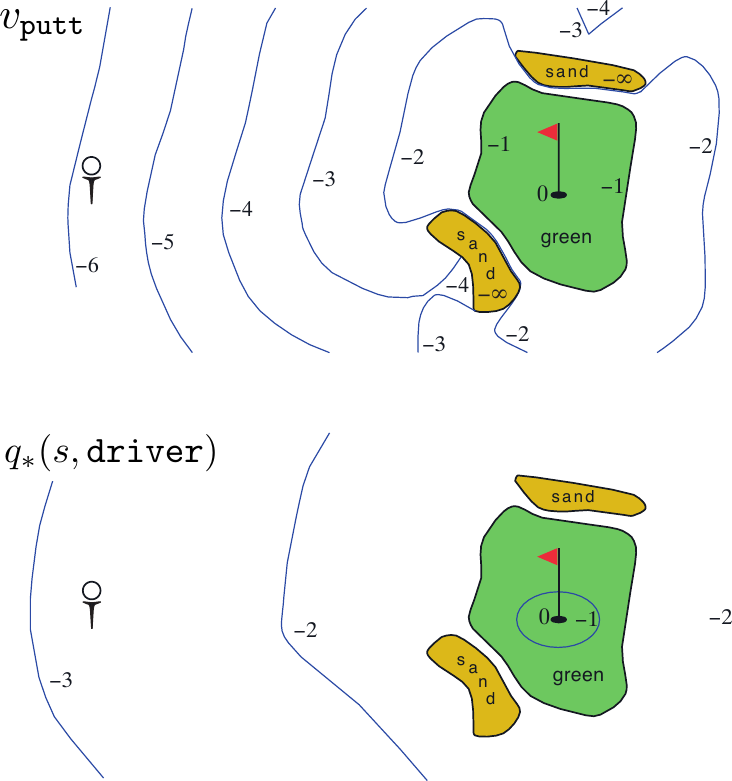
\includegraphics{assets/ch_04/golf_exm.png}

}

\caption{Golf example}

\end{figure}%

}

\caption{\label{fig-golf-exm}Gol example. At top the reward value of
each state (ball curren position).}

\end{figure*}%

\section{Optimal Policies and Optimal Value
Functions}\label{optimal-policies-and-optimal-value-functions}

\section{Optimality and
Approximation}\label{optimality-and-approximation}

\section{Summary}\label{summary-2}

\end{example}

\bookmarksetup{startatroot}

\chapter{Dynamic Programming (DP)}\label{dynamic-programming-dp}

An explanation from ChatGPT. Alright, imagine you have a big puzzle to
solve, but it's too big for you to finish in one go. So, you decide to
break it into smaller puzzles, and you solve each of these small puzzles
one by one. But, here's the clever part: as you solve these small
puzzles, you remember the solutions. That way, if you come across the
same small puzzle again, you don't have to solve it all over again. You
already know the answer! Dynamic programming is like solving a big
puzzle by breaking it into smaller ones and remembering the solutions to
the smaller ones to make solving the big puzzle easier and faster.

\section{Policy Evaluation
(Prediction)}\label{policy-evaluation-prediction}

For this algorithm we iterate as

\begin{equation}\phantomsection\label{eq-policy-evaluation}{
    \begin{aligned}
        v_{k+1}(s) := & \mathbb{E}_{\pi} \left[
            R_{t+1} + \gamma v_k(S_{t+1}) 
            | S_t=s
        \right] 
        \\
        = &
            \sum_{a\in\mathcal{A}(s)}
            \pi(a|s) 
                \sum_{
                    \substack{s^{\prime}\in\mathcal{S},
                    \\ 
                    r \in \mathcal{R}}
                }
                p(s^{\prime}, r |s ,a)
                \left[ 
                    r +\gamma v(s^{\prime})
                \right]
    \end{aligned}
}\end{equation}

To write a sequential computer program to implement iterative policy
evaluation as given by Eq.~\ref{eq-policy-evaluation} you would have to
use two arrays, one for the old values, \(v_k(s)\), and one for the new
values, \(v_{k+1} (s)\). With two arrays, the new values can be computed
one by one from the old values without the old values being changed.

\begin{algorithm}[htb!]
    \caption{Iterative Policy Evaluation, for estimating $V \approx v_{\pi}$ 
    synchronous version}
    \label{alg-test-text-style}
\begin{algorithmic}[1]
        \Require $\pi$, the policy to be evaluated, $\theta$ tolerance precision
        \Ensure $\|v(\cdot)- V(\cdot)\|< \theta$
        \Procedure{Policy-Evaluation}{$\pi$, $\theta$}
            \State $cond \leftarrow$ True
            \While{cond}
            \State $v \leftarrow V$
            \For{$s \in \mathcal{S}$}
                \State $
                        \displaystyle
                        V(s) \leftarrow 
                            \sum_{a}
                                \pi(a|s) 
                                \sum_{
                                    \substack{s^{\prime}\in\mathcal{S},
                                    \\ 
                                    r \in \mathcal{R}}
                                }
                                p(s^{\prime}, r |s ,a)
                                \left[ 
                                    r +\gamma v(s^{\prime})
                                \right]
                    $
            \EndFor
            \State $\Delta \leftarrow \|v -V \|$
            \State $cond \leftarrow (\theta < \Delta)$
        \EndWhile
        \EndProcedure
    \end{algorithmic}
\end{algorithm}

Alternatively, you could use one array and update the values
\texttt{in\ place}, that is, with each new value immediately overwriting
the old one. Then, depending on the order in which the states are
updated, sometimes new values are used instead of old ones on the
right-hand side of Equation~\ref{eq-policy-evaluation} .

\begin{algorithm}[htb!]
    \caption{Iterative Policy Evaluation, for estimating $V \approx v_{\pi}$ 
    in place update version}
    \label{alg-test-text-style}
\begin{algorithmic}[1]
        \Require $\pi$, the policy to be evaluated, $\theta$ tolerance precision
        \Ensure $\|v(\cdot)- V(\cdot)\|< \theta$
        \Procedure{Policy-Evaluation}{$\pi$, $\theta$}
            \State $cond \leftarrow$ True
            \While{cond}
            \State $v \leftarrow V$
            \For{$s \in \mathcal{S}$}
                \State $
                        \displaystyle
                        V(s) \leftarrow 
                            \sum_{a}
                                \pi(a|s) 
                                \sum_{
                                    \substack{s^{\prime}\in\mathcal{S},
                                    \\ 
                                    r \in \mathcal{R}}
                                }
                                p(s^{\prime}, r |s ,a)
                                \left[ 
                                    r +\gamma V(s^{\prime})
                                \right]
                    $
            \EndFor
            \State $\Delta \leftarrow \|v -V \|$
            \State $cond \leftarrow (\theta < \Delta)$
        \EndWhile
        \EndProcedure
    \end{algorithmic}
\end{algorithm}

\begin{example}[]\protect\hypertarget{exm-four-times-four-grid-world}{}\label{exm-four-times-four-grid-world}

The non-terminal states are \(\mathcal{S} = \{1, 2, \dots, 14\}\). There
are four actions possible in each state,
\(\mathcal{A} = \{\verb|up, down, right, left|\}\), which
deterministically cause the corresponding state transitions, except that
actions that would take the agent o↵ the grid in fact leave the state
unchanged. Thus, for instance, \(p(6, 1|5, \verb|right|) = 1\),
~\(p(7, 1|7, \verb1right1) = 1\), and ~
\(p(10, r |5, \verb|right|) = 0\) for all \(r \in \mathcal{R}\). This is
an undiscounted, episodic task. The reward is 1 on all transitions until
the terminal state is reached. The terminal state is shaded in the
figure (although it is shown in two places, it is formally one state).
The expected reward function is thus \(r(s, a, s^{\prime} ) = -1\) for
all states \(s\), \(s^{\prime}\) and actions \(a\). Suppose the agent
follows the equiprobable random policy (all actions equally likely).

\begin{figure*}

\centering{

\begin{figure}[H]

{\centering 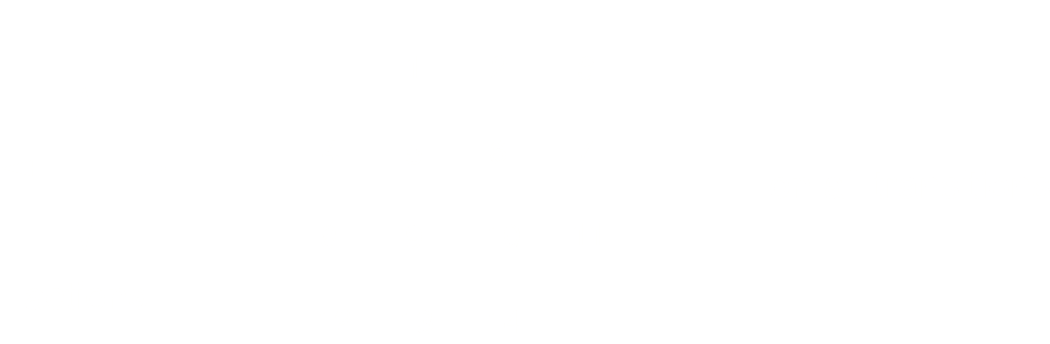
\includegraphics{assets/ch_05/four_times_four_grid_world_exm.png}

}

\caption{4 x 4 grid world example}

\end{figure}%

}

\caption{\label{fig-four_by_four_world_grid_exm}States actions and
rewards for the \(4\times4\) grid-world example.}

\end{figure*}%

\begin{tcolorbox}[enhanced jigsaw, bottomrule=.15mm, opacityback=0, breakable, colframe=quarto-callout-tip-color-frame, left=2mm, rightrule=.15mm, toprule=.15mm, leftrule=.75mm, arc=.35mm, colback=white]

\vspace{-3mm}\textbf{Python implenmentation for the 4 x 4 gridworld example}\vspace{3mm}

\begin{codelisting}[H]

\caption{\texttt{gridworld\_exm\_policy\_ev.py}}

\begin{Shaded}
\begin{Highlighting}[]
\ImportTok{import}\NormalTok{ matplotlib}
\ImportTok{import}\NormalTok{ matplotlib.pyplot }\ImportTok{as}\NormalTok{ plt}
\ImportTok{import}\NormalTok{ numpy }\ImportTok{as}\NormalTok{ np}
\ImportTok{from}\NormalTok{ matplotlib.table }\ImportTok{import}\NormalTok{ Table}

\NormalTok{matplotlib.use(}\StringTok{\textquotesingle{}Agg\textquotesingle{}}\NormalTok{)}

\NormalTok{WORLD\_SIZE }\OperatorTok{=} \DecValTok{4}
\CommentTok{\# left, up, right, down}
\NormalTok{ACTIONS }\OperatorTok{=}\NormalTok{ [np.array([}\DecValTok{0}\NormalTok{, }\OperatorTok{{-}}\DecValTok{1}\NormalTok{]),}
\NormalTok{           np.array([}\OperatorTok{{-}}\DecValTok{1}\NormalTok{, }\DecValTok{0}\NormalTok{]),}
\NormalTok{           np.array([}\DecValTok{0}\NormalTok{, }\DecValTok{1}\NormalTok{]),}
\NormalTok{           np.array([}\DecValTok{1}\NormalTok{, }\DecValTok{0}\NormalTok{])]}
\NormalTok{ACTION\_PROB }\OperatorTok{=} \FloatTok{0.25}


\KeywordTok{def}\NormalTok{ is\_terminal(state):}
\NormalTok{    x, y }\OperatorTok{=}\NormalTok{ state}
    \ControlFlowTok{return}\NormalTok{ (x }\OperatorTok{==} \DecValTok{0} \KeywordTok{and}\NormalTok{ y }\OperatorTok{==} \DecValTok{0}\NormalTok{) }\KeywordTok{or}\NormalTok{ (x }\OperatorTok{==}\NormalTok{ WORLD\_SIZE }\OperatorTok{{-}} \DecValTok{1} \KeywordTok{and}\NormalTok{ y }\OperatorTok{==}\NormalTok{ WORLD\_SIZE }\OperatorTok{{-}} \DecValTok{1}\NormalTok{)}


\KeywordTok{def}\NormalTok{ step(state, action):}
    \ControlFlowTok{if}\NormalTok{ is\_terminal(state):}
        \ControlFlowTok{return}\NormalTok{ state, }\DecValTok{0}

\NormalTok{    next\_state }\OperatorTok{=}\NormalTok{ (np.array(state) }\OperatorTok{+}\NormalTok{ action).tolist()}
\NormalTok{    x, y }\OperatorTok{=}\NormalTok{ next\_state}

    \ControlFlowTok{if}\NormalTok{ x }\OperatorTok{\textless{}} \DecValTok{0} \KeywordTok{or}\NormalTok{ x }\OperatorTok{\textgreater{}=}\NormalTok{ WORLD\_SIZE }\KeywordTok{or}\NormalTok{ y }\OperatorTok{\textless{}} \DecValTok{0} \KeywordTok{or}\NormalTok{ y }\OperatorTok{\textgreater{}=}\NormalTok{ WORLD\_SIZE:}
\NormalTok{        next\_state }\OperatorTok{=}\NormalTok{ state}

\NormalTok{    reward }\OperatorTok{=} \OperatorTok{{-}}\DecValTok{1}
    \ControlFlowTok{return}\NormalTok{ next\_state, reward}


\KeywordTok{def}\NormalTok{ draw\_image(image):}
\NormalTok{    fig, ax }\OperatorTok{=}\NormalTok{ plt.subplots()}
\NormalTok{    ax.set\_axis\_off()}
\NormalTok{    tb }\OperatorTok{=}\NormalTok{ Table(ax, bbox}\OperatorTok{=}\NormalTok{[}\DecValTok{0}\NormalTok{, }\DecValTok{0}\NormalTok{, }\DecValTok{1}\NormalTok{, }\DecValTok{1}\NormalTok{])}

\NormalTok{    nrows, ncols }\OperatorTok{=}\NormalTok{ image.shape}
\NormalTok{    width, height }\OperatorTok{=} \FloatTok{1.0} \OperatorTok{/}\NormalTok{ ncols, }\FloatTok{1.0} \OperatorTok{/}\NormalTok{ nrows}

    \CommentTok{\# Add cells}
    \ControlFlowTok{for}\NormalTok{ (i, j), val }\KeywordTok{in}\NormalTok{ np.ndenumerate(image):}
\NormalTok{        tb.add\_cell(i, j, width, height, text}\OperatorTok{=}\NormalTok{val,}
\NormalTok{                    loc}\OperatorTok{=}\StringTok{\textquotesingle{}center\textquotesingle{}}\NormalTok{, facecolor}\OperatorTok{=}\StringTok{\textquotesingle{}white\textquotesingle{}}\NormalTok{)}

        \CommentTok{\# Row and column labels...}
    \ControlFlowTok{for}\NormalTok{ i }\KeywordTok{in} \BuiltInTok{range}\NormalTok{(}\BuiltInTok{len}\NormalTok{(image)):}
\NormalTok{        tb.add\_cell(i, }\OperatorTok{{-}}\DecValTok{1}\NormalTok{, width, height, text}\OperatorTok{=}\NormalTok{i}\OperatorTok{+}\DecValTok{1}\NormalTok{, loc}\OperatorTok{=}\StringTok{\textquotesingle{}right\textquotesingle{}}\NormalTok{,}
\NormalTok{                    edgecolor}\OperatorTok{=}\StringTok{\textquotesingle{}none\textquotesingle{}}\NormalTok{, facecolor}\OperatorTok{=}\StringTok{\textquotesingle{}none\textquotesingle{}}\NormalTok{)}
\NormalTok{        tb.add\_cell(}\OperatorTok{{-}}\DecValTok{1}\NormalTok{, i, width, height}\OperatorTok{/}\DecValTok{2}\NormalTok{, text}\OperatorTok{=}\NormalTok{i}\OperatorTok{+}\DecValTok{1}\NormalTok{, loc}\OperatorTok{=}\StringTok{\textquotesingle{}center\textquotesingle{}}\NormalTok{,}
\NormalTok{                    edgecolor}\OperatorTok{=}\StringTok{\textquotesingle{}none\textquotesingle{}}\NormalTok{, facecolor}\OperatorTok{=}\StringTok{\textquotesingle{}none\textquotesingle{}}\NormalTok{)}
\NormalTok{    ax.add\_table(tb)}


\KeywordTok{def}\NormalTok{ compute\_state\_value(in\_place}\OperatorTok{=}\VariableTok{True}\NormalTok{, discount}\OperatorTok{=}\FloatTok{1.0}\NormalTok{):}
\NormalTok{    new\_state\_values }\OperatorTok{=}\NormalTok{ np.zeros((WORLD\_SIZE, WORLD\_SIZE))}
\NormalTok{    iteration }\OperatorTok{=} \DecValTok{0}
    \ControlFlowTok{while} \VariableTok{True}\NormalTok{:}
        \ControlFlowTok{if}\NormalTok{ in\_place:}
\NormalTok{            state\_values }\OperatorTok{=}\NormalTok{ new\_state\_values}
        \ControlFlowTok{else}\NormalTok{:}
\NormalTok{            state\_values }\OperatorTok{=}\NormalTok{ new\_state\_values.copy()}
\NormalTok{        old\_state\_values }\OperatorTok{=}\NormalTok{ state\_values.copy()}

        \ControlFlowTok{for}\NormalTok{ i }\KeywordTok{in} \BuiltInTok{range}\NormalTok{(WORLD\_SIZE):}
            \ControlFlowTok{for}\NormalTok{ j }\KeywordTok{in} \BuiltInTok{range}\NormalTok{(WORLD\_SIZE):}
\NormalTok{                value }\OperatorTok{=} \DecValTok{0}
                \ControlFlowTok{for}\NormalTok{ action }\KeywordTok{in}\NormalTok{ ACTIONS:}
\NormalTok{                    (next\_i, next\_j), reward }\OperatorTok{=}\NormalTok{ step([i, j], action)}
\NormalTok{                    value }\OperatorTok{+=}\NormalTok{ ACTION\_PROB }\OperatorTok{*}\NormalTok{ (reward }\OperatorTok{+}\NormalTok{ discount }\OperatorTok{*}\NormalTok{ state\_values[next\_i, next\_j])}
\NormalTok{                new\_state\_values[i, j] }\OperatorTok{=}\NormalTok{ value}

\NormalTok{        max\_delta\_value }\OperatorTok{=} \BuiltInTok{abs}\NormalTok{(old\_state\_values }\OperatorTok{{-}}\NormalTok{ new\_state\_values).}\BuiltInTok{max}\NormalTok{()}
        \ControlFlowTok{if}\NormalTok{ max\_delta\_value }\OperatorTok{\textless{}} \FloatTok{1e{-}4}\NormalTok{:}
            \ControlFlowTok{break}

\NormalTok{        iteration }\OperatorTok{+=} \DecValTok{1}

    \ControlFlowTok{return}\NormalTok{ new\_state\_values, iteration}

\KeywordTok{def}\NormalTok{ figure\_4\_1():}
    \CommentTok{\# While the author suggests using in{-}place iterative policy evaluation,}
    \CommentTok{\# Figure 4.1 actually uses out{-}of{-}place version.}
\NormalTok{    \_, asycn\_iteration }\OperatorTok{=}\NormalTok{ compute\_state\_value(in\_place}\OperatorTok{=}\VariableTok{True}\NormalTok{)}
\NormalTok{    values, sync\_iteration }\OperatorTok{=}\NormalTok{ compute\_state\_value(in\_place}\OperatorTok{=}\VariableTok{False}\NormalTok{)}
\NormalTok{    draw\_image(np.}\BuiltInTok{round}\NormalTok{(values, decimals}\OperatorTok{=}\DecValTok{2}\NormalTok{))}
    \BuiltInTok{print}\NormalTok{(}\StringTok{\textquotesingle{}In{-}place: }\SpecialCharTok{\{\}}\StringTok{ iterations\textquotesingle{}}\NormalTok{.}\BuiltInTok{format}\NormalTok{(asycn\_iteration))}
    \BuiltInTok{print}\NormalTok{(}\StringTok{\textquotesingle{}Synchronous: }\SpecialCharTok{\{\}}\StringTok{ iterations\textquotesingle{}}\NormalTok{.}\BuiltInTok{format}\NormalTok{(sync\_iteration))}

\NormalTok{    plt.savefig(}\StringTok{\textquotesingle{}../images/figure\_4\_1.png\textquotesingle{}}\NormalTok{)}
\NormalTok{    plt.close()}


\ControlFlowTok{if} \VariableTok{\_\_name\_\_} \OperatorTok{==} \StringTok{\textquotesingle{}\_\_main\_\_\textquotesingle{}}\NormalTok{:}
\NormalTok{    figure\_4\_1()}
\end{Highlighting}
\end{Shaded}

\end{codelisting}

\end{tcolorbox}

\end{example}

\section{Policy Improvement}\label{policy-improvement}

Our reason for computing the value function for a policy is to help find
better policies. Suppose we have determined the value function
\(v_{\pi}\) for an arbitrary deterministic policy \(\pi\). For some
state \(s\) we would like to know whether or not we should change the
policy to deterministically choose an action \(a\) such that \[
    a 
    \neq \pi(s).
\]

Becouse we know how good is to follow the current policy \(\pi\) from
\(s\)--that is \(v_{\pi}(s)\)--we can estimate if it better or not to
change to a new policy \(\pi^{\prime}\) which is equal the the original
policy \(\pi\) except at state \(s\). To this end we can sellect
\(a = \pi^{\prime}(s)\) always \(s\) appears and there after use the
original policy \(\pi\). The new value of this argument results

\[
\begin{aligned}
    q_{\pi}(s, a) 
        :=& 
            \mathbb{E} 
                \left[
                    R_{t+1} + \gamma v_{\pi}(S_{t+1})
                    | S_t=s ,A_t=a
                \right]
        \\
        =&
            \sum_{s^{\prime},r}
                p(s^{\prime}, r | s,a)
                \left[
                    r + \gamma v_{\pi}(s^{\prime})
                \right].
    \end{aligned}
\]

Regarding this line of thinking we have the following result

\begin{theorem}[policy
improvement]\protect\hypertarget{thm-policy-improvement}{}\label{thm-policy-improvement}

~

\end{theorem}

\section{Policy Iteration}\label{policy-iteration}

\section{Value Iteration}\label{value-iteration-1}

\section{Asynchronous Dynamic
Programming}\label{asynchronous-dynamic-programming}

\section{Generalized Policy
Iteration}\label{generalized-policy-iteration}

\section{Efficiency of Dynamic
Programming}\label{efficiency-of-dynamic-programming}

\section{Summary}\label{summary-3}

\bookmarksetup{startatroot}

\chapter{Applications}\label{applications}

\section{Recycling Robot}\label{recycling-robot}

\section{A robot with randomly moves in a grid
world.}\label{a-robot-with-randomly-moves-in-a-grid-world.}

\bookmarksetup{startatroot}

\chapter{Project proposal}\label{project-proposal}

\bookmarksetup{startatroot}

\chapter{Formulation and reinforcement learning solution to a
problem}\label{formulation-and-reinforcement-learning-solution-to-a-problem}

of a sequence of decisions.

\bookmarksetup{startatroot}

\chapter{Bases}\label{bases}

\begin{itemize}
\tightlist
\item
  The sequence of decision must be based on a finite Markov decision
  Process.

  \begin{itemize}
  \tightlist
  \item
    The space of states and action must to be finite and discrete.
  \end{itemize}
\end{itemize}

\section{}\label{section}

\section{Death line: December 08,
2024-23:59:00}\label{death-line-december-08-2024-235900}

\section{Sub-products}\label{sub-products}

\begin{longtable}[]{@{}lc@{}}
\toprule\noalign{}
\textbf{Death lines} & \\
\midrule\noalign{}
\endhead
\bottomrule\noalign{}
\endlastfoot
Stage 01 & \textbf{November 02, 2024-23:59} \\
Stage 02 & \textbf{December 05, 2024-23:59} \\
\end{longtable}

\subsection{Stage 01: Quarto book with MDP
formulation}\label{stage-01-quarto-book-with-mdp-formulation}

\begin{itemize}
\item
  The page must encloses the report according to the template
  \texttt{rl\_bookdown\_prg.qmd}

  \begin{itemize}
  \tightlist
  \item
    Introduction
  \item
    Formulation of the Mrakov decision process
  \item
    Model dynamics
  \item
    Description and justification of the Cost (reward)
  \item
    Justification of the actions
  \end{itemize}
\item
  Must include

  \begin{itemize}
  \item
    Figures to illustrates the behavior of the regarding elements:

    \begin{enumerate}
    \def\labelenumi{\arabic{enumi}.}
    \tightlist
    \item
      Policy
    \item
      Reward
    \item
      Value function eventuated for a one state-action and transition.
    \item
      Environmental model
    \end{enumerate}
  \item
    References via bibtex.
  \item
    Output compilation for HTML and PDF formats.
  \item
    The compiled version has to be mounted ing GitHub or Quarto Pub
  \end{itemize}
\end{itemize}

\subsection{Stage 02: Python code
Implementation}\label{stage-02-python-code-implementation}

\begin{itemize}
\tightlist
\item
  Only code whit out running errors wold be accepted
\item
  Code must follows the style guide from PEP 08
\item
  All functions must include doc-strings
\item
  Extras:
\item
  Packing and Documentation \texttt{extra\ 200\ xps}
\end{itemize}

\subsection{Stage 03: Video
Presentation}\label{stage-03-video-presentation}

A video mounted in you-tube of at most 20 min with results and insight
of your project

\section{Suggested project list:}\label{suggested-project-list}

\begin{enumerate}
\def\labelenumi{\arabic{enumi}.}
\tightlist
\item
  Reinforcement learning simulation of the TIC-TAC-TOE Game with SARSA
  or Q-learning Algorithms Bilgin (\citeproc{ref-Bilgin2020}{2020})
\item
  The movement of a Recycling Robot Bilgin
  (\citeproc{ref-Bilgin2020}{2020})
\item
  The replacement of a bus engine (\citeproc{ref-Rust1987}{Rust 1987})
  from (see pd.pdf, p.130 \citeproc{ref-Starchursky2024}{Stachurski.
  2024})
\item
  Optimal Inventories (see dp.pdf, p.~147
  \citeproc{ref-Starchursky2024}{Stachurski. 2024})
\item
  Multi-Armed Bandits Bilgin (\citeproc{ref-Bilgin2020}{2020})
\end{enumerate}

\section{Project Lits}\label{project-lits}

\begin{longtable}[]{@{}
  >{\raggedright\arraybackslash}p{(\columnwidth - 4\tabcolsep) * \real{0.3333}}
  >{\raggedright\arraybackslash}p{(\columnwidth - 4\tabcolsep) * \real{0.3333}}
  >{\raggedright\arraybackslash}p{(\columnwidth - 4\tabcolsep) * \real{0.3333}}@{}}
\caption{Project list}\tabularnewline
\toprule\noalign{}
\begin{minipage}[b]{\linewidth}\raggedright
Project
\end{minipage} & \begin{minipage}[b]{\linewidth}\raggedright
Author
\end{minipage} & \begin{minipage}[b]{\linewidth}\raggedright
Reference
\end{minipage} \\
\midrule\noalign{}
\endfirsthead
\toprule\noalign{}
\begin{minipage}[b]{\linewidth}\raggedright
Project
\end{minipage} & \begin{minipage}[b]{\linewidth}\raggedright
Author
\end{minipage} & \begin{minipage}[b]{\linewidth}\raggedright
Reference
\end{minipage} \\
\midrule\noalign{}
\endhead
\bottomrule\noalign{}
\endlastfoot
Dynamic Portfolio Analysis & GABRIEL MIRANDA GAMEZ & (Sec. 4.3,
\citeproc{ref-Bertsekas2005}{Bertsekas 2005}) \\
Learning the Best Diabetes Medication & EDGAR EVERARDO MARTINEZ GARCIA &
(Ch.4 4, \citeproc{ref-powell2022sequential}{Powell et al. 2022}) \\
A MDP model for the collective behavior in vaccination campaigns &
IRASEMA PEDROZA MEZA & \\
Modelo de inventario para alimentos pedecederos & DAVID PEÑA PERALTA &
(\citeproc{ref-Starchursky2024}{Stachurski. 2024}) \\
A inventory model & JAZMIN SARAHI FLORES GOMEZ &
(\citeproc{ref-levhari1982great}{Levhari and Mirman 1982}) \\
\end{longtable}

\section{Configuration to build with Spanish
language}\label{configuration-to-build-with-spanish-language}

Adapt to your project accordingly to your .png files another sources.

\begin{codelisting}

\caption{\texttt{\_quarto.yml}}

\begin{Shaded}
\begin{Highlighting}[]
\AttributeTok{  }\FunctionTok{project}\KeywordTok{:}
\AttributeTok{  }\FunctionTok{type}\KeywordTok{:}\AttributeTok{ book}
\AttributeTok{  }\FunctionTok{output{-}dir}\KeywordTok{:}\AttributeTok{ \_book}

\FunctionTok{website}\KeywordTok{:}
\AttributeTok{  }\FunctionTok{favicon}\KeywordTok{:}\AttributeTok{ FCFMLOGO.png}
\AttributeTok{  }\FunctionTok{reader{-}mode}\KeywordTok{:}\AttributeTok{ }\CharTok{true}
\AttributeTok{  }\FunctionTok{search}\KeywordTok{:}
\AttributeTok{    }\FunctionTok{location}\KeywordTok{:}\AttributeTok{ sidebar}
\AttributeTok{    }\FunctionTok{type}\KeywordTok{:}\AttributeTok{ overlay}
\AttributeTok{  }\FunctionTok{comments}\KeywordTok{:}
\AttributeTok{    }\FunctionTok{hypothesis}\KeywordTok{:}\AttributeTok{ }\CharTok{true}

\FunctionTok{book}\KeywordTok{:}
\AttributeTok{  }\FunctionTok{title}\KeywordTok{:}\AttributeTok{ }\StringTok{"Análisis comparativo del desempeño en métodos para el pronóstico de series temporales"}
\AttributeTok{  }\FunctionTok{reader{-}mode}\KeywordTok{:}\AttributeTok{ }\CharTok{true}
\AttributeTok{  }\FunctionTok{language}\KeywordTok{:}\AttributeTok{ es}
\AttributeTok{  }\FunctionTok{date}\KeywordTok{:}\AttributeTok{ }\StringTok{"02/14/2024"}
\AttributeTok{  }\FunctionTok{output{-}file}\KeywordTok{:}\AttributeTok{ }\StringTok{"Tesis\_JSLG"}
\CommentTok{  \# image: logofcfm.png}
\CommentTok{  \# cover{-}image: FCFMLOGO.png}
\AttributeTok{  }\FunctionTok{sharing}\KeywordTok{:}\AttributeTok{ }\KeywordTok{[}\AttributeTok{twitter}\KeywordTok{,}\AttributeTok{ facebook}\KeywordTok{]}
\AttributeTok{  }\FunctionTok{downloads}\KeywordTok{:}\AttributeTok{ }\KeywordTok{[}\AttributeTok{pdf}\KeywordTok{,}\AttributeTok{ epub}\KeywordTok{]}
\CommentTok{  \# favicon: logofcfm.png}
\AttributeTok{  }\FunctionTok{sidebar}\KeywordTok{:}
\CommentTok{  \#  logo: LOGO50.png}
\AttributeTok{    }\FunctionTok{style}\KeywordTok{:}\AttributeTok{ floating}
\AttributeTok{    }\FunctionTok{collapse{-}level}\KeywordTok{:}\AttributeTok{ }\DecValTok{2}
\AttributeTok{    }\FunctionTok{border}\KeywordTok{:}\AttributeTok{ }\CharTok{true}
\AttributeTok{    }\FunctionTok{search}\KeywordTok{:}\AttributeTok{ }\CharTok{true}
\AttributeTok{  }\FunctionTok{open{-}graph}\KeywordTok{:}\AttributeTok{ }\CharTok{true}
\AttributeTok{  }\FunctionTok{twitter{-}card}\KeywordTok{:}\AttributeTok{ }\CharTok{true}
\CommentTok{  \#repo{-}url: https://github.com/Jennlg/Tesis}
\AttributeTok{  }\FunctionTok{repo{-}actions}\KeywordTok{:}\AttributeTok{ }\KeywordTok{[}\AttributeTok{edit}\KeywordTok{,}\AttributeTok{ issue}\KeywordTok{,}\AttributeTok{ source}\KeywordTok{]}
\AttributeTok{  }\FunctionTok{page{-}navigation}\KeywordTok{:}\AttributeTok{ }\CharTok{true}
\AttributeTok{  }\FunctionTok{chapters}\KeywordTok{:}
\AttributeTok{    }\KeywordTok{{-}}\AttributeTok{ index.qmd}
\AttributeTok{    }\KeywordTok{{-}}\AttributeTok{ intro.qmd}
\AttributeTok{    }\KeywordTok{{-}}\AttributeTok{ objetivos.qmd}

\AttributeTok{    }\KeywordTok{{-}}\AttributeTok{ }\FunctionTok{part}\KeywordTok{:}\AttributeTok{ }\StringTok{\textquotesingle{}Preliminares\textquotesingle{}}
\AttributeTok{      }\FunctionTok{chapters}\KeywordTok{:}
\AttributeTok{        }\KeywordTok{{-}}\AttributeTok{ tconjuntos.qmd}
\AttributeTok{        }\KeywordTok{{-}}\AttributeTok{ probabilidad.qmd}
\AttributeTok{        }\KeywordTok{{-}}\AttributeTok{ estadistica.qmd}
\AttributeTok{        }\KeywordTok{{-}}\AttributeTok{ procesos.qmd}
\AttributeTok{    }\KeywordTok{{-}}\AttributeTok{ }\FunctionTok{part}\KeywordTok{:}\AttributeTok{ }\StringTok{\textquotesingle{}Series de tiempo\textquotesingle{}}
\AttributeTok{      }\FunctionTok{chapters}\KeywordTok{:}
\AttributeTok{        }\KeywordTok{{-}}\AttributeTok{ series.qmd}
\AttributeTok{    }\KeywordTok{{-}}\AttributeTok{ }\FunctionTok{part}\KeywordTok{:}\AttributeTok{ }\StringTok{\textquotesingle{}Redes neuronales\textquotesingle{}}
\AttributeTok{      }\FunctionTok{chapters}\KeywordTok{:}
\AttributeTok{        }\KeywordTok{{-}}\AttributeTok{ redes.qmd}
\AttributeTok{    }\KeywordTok{{-}}\AttributeTok{ }\FunctionTok{part}\KeywordTok{:}\AttributeTok{ estudio.qmd}
\AttributeTok{      }\FunctionTok{chapters}\KeywordTok{:}
\AttributeTok{        }\KeywordTok{{-}}\AttributeTok{ metodologia.qmd}
\AttributeTok{        }\KeywordTok{{-}}\AttributeTok{ confirmados.qmd}
\AttributeTok{        }\KeywordTok{{-}}\AttributeTok{ muertes.qmd}
\AttributeTok{    }\KeywordTok{{-}}\AttributeTok{ conclusiones.qmd}

\AttributeTok{    }\KeywordTok{{-}}\AttributeTok{ references.qmd}

\FunctionTok{comments}\KeywordTok{:}
\AttributeTok{    }\FunctionTok{hypothesis}\KeywordTok{:}\AttributeTok{ }\CharTok{true}

\FunctionTok{bibliography}\KeywordTok{:}\AttributeTok{ references.bib}

\FunctionTok{format}\KeywordTok{:}
\AttributeTok{  }\FunctionTok{html}\KeywordTok{:}
\AttributeTok{    }\FunctionTok{theme}\KeywordTok{:}
\AttributeTok{      }\FunctionTok{dark}\KeywordTok{:}\AttributeTok{ darkly}
\AttributeTok{      }\FunctionTok{light}\KeywordTok{:}\AttributeTok{ cerulean}
\AttributeTok{    }\FunctionTok{highlight{-}style}\KeywordTok{:}\AttributeTok{ a11y}
\AttributeTok{    }\FunctionTok{lang}\KeywordTok{:}\AttributeTok{ es}
\AttributeTok{    }\FunctionTok{html{-}math{-}method}\KeywordTok{:}\AttributeTok{ mathjax}
\AttributeTok{    }\FunctionTok{grid}\KeywordTok{:}
\AttributeTok{      }\FunctionTok{sidebar{-}width}\KeywordTok{:}\AttributeTok{ 300px}
\AttributeTok{      }\FunctionTok{body{-}width}\KeywordTok{:}\AttributeTok{ 900px}
\AttributeTok{      }\FunctionTok{margin{-}width}\KeywordTok{:}\AttributeTok{ 300px}
\AttributeTok{      }\FunctionTok{gutter{-}width}\KeywordTok{:}\AttributeTok{ 1.5rem}
\AttributeTok{    }\FunctionTok{code{-}copy}\KeywordTok{:}\AttributeTok{ }\CharTok{true}
\AttributeTok{    }\FunctionTok{code{-}fold}\KeywordTok{:}\AttributeTok{ }\CharTok{true}
\AttributeTok{  }\FunctionTok{pdf}\KeywordTok{:}
\AttributeTok{    }\FunctionTok{lang}\KeywordTok{:}\AttributeTok{ es}
\AttributeTok{    }\FunctionTok{include{-}in{-}header}\KeywordTok{:}
\AttributeTok{      }\KeywordTok{{-}}\AttributeTok{ packa.tex}
\AttributeTok{    }\FunctionTok{template{-}partials}\KeywordTok{:}
\AttributeTok{      }\KeywordTok{{-}}\AttributeTok{ before{-}body.tex}
\AttributeTok{    }\FunctionTok{documentclass}\KeywordTok{:}\AttributeTok{ scrreprt}
\AttributeTok{    }\FunctionTok{papersize}\KeywordTok{:}\AttributeTok{ us{-}letter}
\CommentTok{    \#titlegraphic: FCFMLOGO.png}
\AttributeTok{    }\FunctionTok{institution}\KeywordTok{:}\AttributeTok{ Universidad Autónoma de Chiapas}
\AttributeTok{    }\FunctionTok{email}\KeywordTok{:}\AttributeTok{ jennifer.lopez67@unach.mx}
\AttributeTok{    }\FunctionTok{keep{-}tex}\KeywordTok{:}\AttributeTok{ }\CharTok{true}
\AttributeTok{  }\FunctionTok{epub}\KeywordTok{:}
\AttributeTok{    }\FunctionTok{cover{-}image}\KeywordTok{:}\AttributeTok{ FCFMLOGO.png}
\FunctionTok{editor}\KeywordTok{:}\AttributeTok{ visual}
\end{Highlighting}
\end{Shaded}

\end{codelisting}

We also need the following .tex in the root folder

\begin{Shaded}
\begin{Highlighting}[]
\BuiltInTok{\textbackslash{}usepackage}\NormalTok{\{}\ExtensionTok{upgreek}\NormalTok{\}}
\BuiltInTok{\textbackslash{}usepackage}\NormalTok{\{}\ExtensionTok{amsmath}\NormalTok{\}}
\BuiltInTok{\textbackslash{}usepackage}\NormalTok{\{}\ExtensionTok{amssymb}\NormalTok{\}}
\FunctionTok{\textbackslash{}newcommand}\NormalTok{\{}\ExtensionTok{\textbackslash{}dashedbox}\NormalTok{\}[1]\{}
  \KeywordTok{\textbackslash{}begin}\NormalTok{\{}\ExtensionTok{tikzpicture}\NormalTok{\}}
    \FunctionTok{\textbackslash{}node}\NormalTok{[draw, dashed, rounded corners=5pt, inner sep=10pt] \{}
      \KeywordTok{\textbackslash{}begin}\NormalTok{\{}\ExtensionTok{minipage}\NormalTok{\}\{0.8}\FunctionTok{\textbackslash{}textwidth}\NormalTok{\} }\CommentTok{\% Establece el ancho del minipage}
\NormalTok{        \#1}
      \KeywordTok{\textbackslash{}end}\NormalTok{\{}\ExtensionTok{minipage}\NormalTok{\}}
\NormalTok{    \};}
  \KeywordTok{\textbackslash{}end}\NormalTok{\{}\ExtensionTok{tikzpicture}\NormalTok{\}}
\NormalTok{\}}
\end{Highlighting}
\end{Shaded}

\bookmarksetup{startatroot}

\chapter{Evaluation Rubric}\label{evaluation-rubric}

\bookmarksetup{startatroot}

\chapter{List of Home Works and due
dates}\label{list-of-home-works-and-due-dates}

\section{Homework 001 due date: september 20,
2024-12:00:00}\label{homework-001-due-date-september-20-2024-120000}

\begin{exercise}[]\protect\hypertarget{exr-hw_001_01}{}\label{exr-hw_001_01}

Read (Sec 1.1, pp 1-2 \citeproc{ref-Sutton2018}{Sutton and Barto 2018})
and answer the following.

Explain why Reinforcement Learning differs for supervised and
unsupervised learning.

\end{exercise}

\begin{exercise}[]\protect\hypertarget{exr-hw_001_02}{}\label{exr-hw_001_02}

See the first Steve Brunton's youtube video about
\href{https://www.youtube.com/watch?v=0MNVhXEX9to&list=PLMrJAkhIeNNQe1JXNvaFvURxGY4gE9k74}{Reinforcement
Learning}. Then accordingly to its presentation explain what is the
meaning of the following expression:

\[
  V_{\pi}(s) = \mathbb{E}
 \left(
   \sum_{t} \gamma ^ {t} r_t | s_0 = s
 \right).
\]

\end{exercise}

\begin{exercise}[]\protect\hypertarget{exr-hw_001_03}{}\label{exr-hw_001_03}

Form (see \citeproc{ref-Sutton2018}{Sutton and Barto 2018, sec. 1.7})
obtain a time line pear year from 1950 to 2012.

Use the following format
\href{https://kim.quarto.pub/milestones--bar-timelines/}{see
https://kim.quarto.pub/milestones--bar-timelines/}

\end{exercise}

\begin{exercise}[]\protect\hypertarget{exr-hw_001_04}{}\label{exr-hw_001_04}

Consider the following \textbf{consumption--saving} problem with
dynamics \[ 
  x_{k+1}
  = (1+r)(x_k-a_k),\qquad k=0,1,\ldots,N-1, 
\] and utility function

\[
  \beta^N(x_N)^{1-\gamma} 
    + \sum_{k=0}^{N-1}\beta^k (a_k)^{1-\gamma}. 
\]

Show that the value functions of the DP algorithm take the form
\[J_k(x)=A_k\beta^kx^{1-\gamma},\] where \(A_N=1\) and for
\(k=N-1,\ldots,0\),

\[  A_k = [1 + ((1+r)\beta A_{k+1})^{1/\gamma} ]^\gamma.  \] Show also
that the optimal policies are \(h_k(x)=A_k^{-1/\gamma} x\). for
\(k=N-1,\ldots,0\).

\end{exercise}

\begin{exercise}[]\protect\hypertarget{exr-hw_001_05}{}\label{exr-hw_001_05}

Consider now the infinite--horizon version of the above
consumption--saving problem.

\begin{enumerate}
\def\labelenumi{\roman{enumi})}
\item
  Write down the associated Bellman equation.
\item
  Argue why a solution to the Bellman equation should be of the form
  \[v(x)=cx^{1-\gamma},\] where \(c\) is constant. Find the constant
  \(c\) and the stationary optimal policy \footnote{Hint: Insert
    \(v(x)=cx^{1-\gamma}\) into the Bellman equation and solve the
    minimization problem.}.
\end{enumerate}

\end{exercise}

\begin{exercise}[]\protect\hypertarget{exr-hw_001_06}{}\label{exr-hw_001_06}

Let \(\{\xi_k\}\) be a sequence of iid random variables such that
\(E[\xi]=0\) and \(E[\xi^2]=d\). Consider the dynamics \[ 
  x_{k+1} = x_k + a_k + \xi_k, \qquad 
  k= 0,1,2,\ldots, 
\] and the discounted cost \[
  E \sum \beta^k(a_k^2+x_k^2).
\]

\begin{enumerate}
\def\labelenumi{\roman{enumi})}
\item
  Write down the associated Bellman equation.
\item
  Conjecture that the solution to the Bellman equation takes the form
  \(v(x)=ax^2+b\), where \(a\) and \(b\) are constant.
\item
  Determine the constants \(a\) and \(b\).
\item
  Conjecture that the solution to the Bellman equation takes the form
  \(v(x)=ax^2+b\), where \(a\) and \(b\) are constant. Determine the
  constants \(a\) and \(b\).
\end{enumerate}

\end{exercise}

\section{Homework 002 due date: October 25,
2024-12:00:00}\label{homework-002-due-date-october-25-2024-120000}

\begin{exercise}[]\protect\hypertarget{exr-hw_002_01}{}\label{exr-hw_002_01}

Make the docstrings regarding all python source code for each reported
script.

\begin{itemize}
\tightlist
\item
  Incremental Implementation
\item
  Optimistic Initial Values
\item
  Upper-Confidence-Bound Action Selection
\item
  Gradient Bandit method
\item
  Scripts for visualization
\end{itemize}

\end{exercise}

\begin{exercise}[]\protect\hypertarget{exr-hw_002_02}{}\label{exr-hw_002_02}

Explain and illustrate the experiments about optimistic initial values.
Include the plots similar to Figure 2.2 from (p.~29,
\citeproc{ref-Sutton2018}{Sutton and Barto 2018}).

\end{exercise}

\begin{exercise}[]\protect\hypertarget{exr-hw_002_03}{}\label{exr-hw_002_03}

Explain and illustrate the experiments about optimistic initial values.
Include the plots similar to Figure 2.3 from (p.~34,
\citeproc{ref-Sutton2018}{Sutton and Barto 2018}).

\end{exercise}

\begin{exercise}[]\protect\hypertarget{exr-hw_002_04}{}\label{exr-hw_002_04}

Explain and describe the experiments about average performance of UCB.
Include the plots similar to Figure 2.4 from (p.~36,
\citeproc{ref-Sutton2018}{Sutton and Barto 2018}).

\end{exercise}

\begin{exercise}[]\protect\hypertarget{exr-hw_002_05}{}\label{exr-hw_002_05}

Explain and describe the experiments about average performance of the
gradient bandit algorithm with and without a reward baseline. Include
the plots similar to Figure 2.5 from (p.~38
\citeproc{ref-Sutton2018}{Sutton and Barto 2018}).

\end{exercise}

\begin{exercise}[]\protect\hypertarget{exr-hw_002_06}{}\label{exr-hw_002_06}

Show that for two actions, the soft-max (Boltzmann or Gibbs)
distribution is equivalent to the logistic, or sigmoid, function
commonly used in statistics and artificial neural networks.

\end{exercise}

\section{Homework 003 due date: November 08,
2024-12:00:00}\label{homework-003-due-date-november-08-2024-120000}

\begin{exercise}[]\protect\hypertarget{exr-hw_003_01}{}\label{exr-hw_003_01}

Suppose \(\gamma= 0.5\) and the following sequence of rewards is
received \(R_1 = 1\),\(R_2 = 2\), \(R_3 = 6\), \(R_4 = 3\), and
\(R_5 = 2\), with \(T = 5\). What are \(G_0 , G_1 , \cdots, G_5\)?
\footnote{Hint: Work backwards.}

\end{exercise}

\begin{exercise}[]\protect\hypertarget{exr--hw_003_02}{}\label{exr--hw_003_02}

Give a table analogous to that in (p.53,
\citeproc{ref-Sutton2018}{Sutton and Barto 2018}), but for
\(p(s_0 , r |s, a)\). It should have columns for \(s\), \(a\), \(s_0\) ,
\(r\), and \(p(s_0 , r |s, a)\), and a row for every 4-tuple for which
\(p(s_0 , r |s, a) > 0\).

\end{exercise}

\begin{exercise}[]\protect\hypertarget{exr--hw_003_03}{}\label{exr--hw_003_03}

If the current state is \(S_t\) , and actions are selected according to
a stochastic policy \(\pi\), then what is the expectation of \(R_{t+1}\)
in terms of \(\pi\) and the four-argument function \(p\) in ((3.2) p.48,
\citeproc{ref-Sutton2018}{Sutton and Barto 2018})?

\end{exercise}

Let the value function of a state \(s\) under a policy \(\pi\) denoted
and defined by \[
\begin{aligned}
    v_{\pi}(s):=  &
        \mathbb{E_{\pi}}
        \left[
            G_t | S_t = s
        \right]
        \\
        = &
        \mathbb{E_{\pi}}
        \left[
            \sum_{k=0}^{\infty}
                R_{t+1+k}
                \Big |
                S_t = s
        \right], \quad \text{for all } s\in \mathcal{S}.
\end{aligned}
\] Similarly we denote and define the value of taking action \(a\) in
state \(s\) under a policy \(\pi\) by \[
\begin{aligned}
    q_{\pi}(s,a):=  &
        \mathbb{E_{\pi}}
        \left[
            G_t | S_t = s, A_t = a
        \right]
        \\
        = &
        \mathbb{E_{\pi}}
        \left[
            \sum_{k=0}^{\infty}
                R_{t+1+k}
                \Big |
                S_t = s, A_t = a
        \right], \quad \text{for all } (s,a) \in \mathcal{S}\times \mathcal{A}(s).
\end{aligned}
\]

\begin{exercise}[]\protect\hypertarget{exr--hw_003_04}{}\label{exr--hw_003_04}

Give an equation for \(v_{\pi}\) in terms of \(q_{\pi}\) and \(\pi\).

\end{exercise}

\begin{exercise}[]\protect\hypertarget{exr--hw_003_05}{}\label{exr--hw_003_05}

~

\begin{enumerate}
\def\labelenumi{\arabic{enumi}.}
\tightlist
\item
  Give an equation for \(q_{\pi}\) in terms of \(v_{\pi}\) and the
  four-argument \(p(\cdot,\cdot|\cdot,\cdot)\)
\item
  Give the Bellman equation for \(q_{\pi}\) for the recycling robot.
\end{enumerate}

\end{exercise}

\begin{exercise}[]\protect\hypertarget{exr--hw_003_06}{}\label{exr--hw_003_06}

Document the numerical experiment regarding to the Gridworld example

\end{exercise}

\bookmarksetup{startatroot}

\chapter{Homework grades}\label{homework-grades}

\bookmarksetup{startatroot}

\chapter*{References}\label{references}
\addcontentsline{toc}{chapter}{References}

\markboth{References}{References}

For the cured R-quarto material see
\url{https://github.com/SaulDiazInfante/intro-quarto-unison-2024}.

\phantomsection\label{refs}
\begin{CSLReferences}{1}{0}
\bibitem[\citeproctext]{ref-Bertsekas2005}
Bertsekas, Dimitri P. 2005. \emph{Dynamic Programming and Optimal
Control. {V}ol. {I}}. Third. Athena Scientific, Belmont, MA.

\bibitem[\citeproctext]{ref-Bilgin2020}
Bilgin, E. 2020. \emph{Mastering Reinforcement Learning with Python:
Build Next-Generation, Self-Learning Models Using Reinforcement Learning
Techniques and Best Practices}. Packt Publishing.
\url{https://books.google.com.mx/books?id=s0MQEAAAQBAJ}.

\bibitem[\citeproctext]{ref-brandimarte2013numerical}
Brandimarte, Paolo. 2013. \emph{Numerical Methods in Finance and
Economics: A MATLAB-Based Introduction}. 2nd ed. Hoboken, New Jersey:
John Wiley \& Sons.

\bibitem[\citeproctext]{ref-Brunton2019}
Brunton, Steven L., and J. Nathan Kutz. 2019. \emph{Data-Driven Science
and Engineering}. Cambridge University Press, Cambridge.
\url{https://doi.org/10.1017/9781108380690}.

\bibitem[\citeproctext]{ref-levhari1982great}
Levhari, DAVID, and Leonard J Mirman. 1982. {``The Great Fish War: An
Example Using a Dynamic Cournot-Nash Solution.''} \emph{Essays in the
Economics of Renewable Resources, LJ Mirman and DF Spulber (Eds.),
North-Holland}, 243--58.

\bibitem[\citeproctext]{ref-powell2022sequential}
Powell, Warren B et al. 2022. {``Sequential Decision Analytics and
Modeling: Modeling with Python.''}

\bibitem[\citeproctext]{ref-Rust1987}
Rust, John. 1987. {``{Optimal Replacement of GMC Bus Engines: An
Empirical Model of Harold Zurcher}.''} \emph{Econometrica} 55 (5): 999.
\url{https://doi.org/10.2307/1911259}.

\bibitem[\citeproctext]{ref-Starchursky2024}
Stachurski., John. 2024. {``Dynamic Programming Volume 1.''}
\emph{GitHub Repository}.
\url{https://github.com/QuantEcon/book-dp1-public}; GitHub.

\bibitem[\citeproctext]{ref-Sutton2018}
Sutton, Richard S., and Andrew G. Barto. 2018. \emph{Reinforcement
Learning: An Introduction}. Second. Adaptive Computation and Machine
Learning. MIT Press, Cambridge, MA.

\bibitem[\citeproctext]{ref-Szepesvari2022}
Szepesvári, Csaba. 2022. \emph{Algorithms for Reinforcement Learning}.
Vol. 9. Synthesis Lectures on Artificial Intelligence and Machine
Learning. Springer, Cham.
\url{https://doi.org/10.1007/978-3-031-01551-9}.

\end{CSLReferences}



\backmatter
\printindex

\end{document}
